\documentclass[12pt, a4paper, oneside]{report}

% --- PACOTES ESSENCIAIS ---
\usepackage[utf8]{inputenc}
\usepackage[T1]{fontenc}
\usepackage{lmodern}
\usepackage[brazil]{babel}
\usepackage{graphicx}
\usepackage{amsmath, amssymb, amsthm}
\usepackage{geometry}
\usepackage{setspace}
\usepackage{booktabs}
\usepackage{caption}
\usepackage{subcaption}
\usepackage{xcolor}
\usepackage{hyperref}
\usepackage{cite}
\usepackage{fancyhdr}
\usepackage{tocbibind}
\usepackage{listings}
\usepackage{siunitx}
\usepackage{float} % Para forçar posição de figuras

% --- CONFIGURAÇÕES DE PÁGINA (ABNT) ---
\geometry{a4paper, left=3cm, right=2cm, top=3cm, bottom=2cm}
\onehalfspacing

% --- CONFIGURAÇÕES DE HIPERLINKS ---
\hypersetup{colorlinks=true, linkcolor=blue, filecolor=magenta, urlcolor=cyan, citecolor=red, pdftitle={Classificação de Supercondutores com Aprendizado de Máquina}, pdfauthor={Lucas Martin De Lucca}}

% --- AMBIENTES MATEMÁTICOS ---
\newtheorem{theorem}{Teorema}[chapter]
\newtheorem{definition}[theorem]{Definição}
\newtheorem{lemma}[theorem]{Lema}

% --- CABEÇALHO E RODAPÉ ---
\pagestyle{fancy}
\fancyhf{}
\fancyhead[L]{\nouppercase{\leftmark}}
\fancyfoot[C]{\thepage}
\setlength{\headheight}{15pt}
\renewcommand{\headrulewidth}{0.4pt}
\renewcommand{\footrulewidth}{0.4pt}

% =============================================================================
\begin{document}

% --- CAPA ---
\begin{titlepage}
    \centering
    \vspace*{1cm}
    {\scshape\Large FUNDAÇÃO UNIVERSIDADE FEDERAL DO ABC \\ Centro de Ciências Naturais e Humanas \\ Curso de Bacharelado em Física}
    \vfill
    {\Huge\bfseries Classificação de Supercondutores Utilizando Técnicas de Aprendizado de Máquina: Uma Abordagem da Física Computacional}
    \vfill
    {\Large\itshape Lucas Martin De Lucca}\\[1cm]
    % TODO: preencher o nome do orientador antes da entrega final
    {\large Orientador: Prof. Dr. [Nome do Orientador]}
    \vfill
    {\large Santo André -- SP \\ 2026}
\end{titlepage}

\newpage\thispagestyle{empty}\mbox{}

% --- RESUMO ---
\newpage
\begin{abstract}
\noindent
A busca por novos materiais supercondutores, especialmente aqueles que exibem o fenômeno a temperaturas mais elevadas, é uma das fronteiras mais ativas da física da matéria condensada. A complexidade dos mecanismos subjacentes, particularmente em supercondutores não convencionais, torna a predição teórica a partir de primeiros princípios uma tarefa computacionalmente custosa e, por vezes, intratável. Este trabalho explora uma abordagem alternativa, fundamentada na física computacional e na ciência de dados, para classificar materiais como supercondutores ou não-supercondutores com base em um conjunto de descritores físicos. Utilizando um banco de dados público contendo mais de 2.400 compostos extraídos do repositório SciDB, foram implementados e avaliados seis modelos de aprendizado de máquina: Random Forest, XGBoost, LightGBM, Support Vector Machine (SVM), Multilayer Perceptron (MLP) e LASSO. A metodologia envolveu pré-processamento rigoroso, otimização de hiperparâmetros via \texttt{RandomizedSearchCV}, controle de \textit{data leakage} via \texttt{GroupShuffleSplit} e análise comparativa estatística (testes de McNemar, Friedman e intervalos bootstrap). Os resultados demonstram a viabilidade da abordagem: o Random Forest alcançou o melhor F1-Score (0.723) com alto \textit{recall} (0.890), enquanto o XGBoost obteve o melhor ROC-AUC (0.724), com o teste de Friedman ($p = 0{,}055$) indicando ausência de diferença estatisticamente significativa entre os modelos a 5\%. Análises de interpretabilidade via SHAP e \textit{Partial Dependence Plots} revelaram que descritores da densidade de estados eletrônicos (DOS) e da estrutura de bandas no nível de Fermi são os mais preditivos, corroborando a intuição física de que a supercondutividade está intrinsecamente ligada ao comportamento dos elétrons na superfície de Fermi. Uma análise de erro mostrou que os modelos têm maior dificuldade em classificar supercondutores convencionais de baixa temperatura crítica ($T_c < 5$ K). Este estudo fornece um modelo preditivo funcional e reforça a sinergia entre o aprendizado de máquina e a física, abrindo caminhos para a triagem acelerada de novos materiais promissores.
\vspace{\baselineskip}

\noindent\textbf{Palavras-chave}: Supercondutividade, Aprendizado de Máquina, Física Computacional, Classificação de Materiais, Teoria BCS.
\end{abstract}

% --- ABSTRACT ---
\newpage
\renewcommand{\abstractname}{Abstract}
\begin{otherlanguage}{english}
\begin{abstract}
\noindent
The search for new superconducting materials, especially those exhibiting the phenomenon at higher temperatures, is one of the most active frontiers in condensed matter physics. The complexity of the underlying mechanisms, particularly in unconventional superconductors, makes theoretical prediction from first principles a computationally expensive and sometimes intractable task. This work explores an alternative approach, grounded in computational physics and data science, to classify materials as superconductors or non-superconductors based on a set of physical descriptors. Using a public database containing over 2,400 compounds extracted from the SciDB repository, six machine learning models were implemented and evaluated: Random Forest, XGBoost, LightGBM, Support Vector Machine (SVM), Multilayer Perceptron (MLP), and LASSO. The methodology involved rigorous preprocessing, hyperparameter optimization via \texttt{RandomizedSearchCV}, data leakage control via \texttt{GroupShuffleSplit}, and statistical comparative analysis (McNemar, Friedman, and bootstrap confidence intervals). The results demonstrate the feasibility of the approach: Random Forest achieved the best F1-Score (0.723) with high recall (0.890), while XGBoost obtained the best ROC-AUC (0.724), with Friedman's test ($p = 0.055$) indicating no statistically significant difference between models at 5\%. Interpretability analyses via SHAP and Partial Dependence Plots revealed that descriptors of the electronic density of states (DOS) and the band structure at the Fermi level are the most predictive, corroborating the physical intuition that superconductivity is intrinsically linked to the behavior of electrons at the Fermi surface. An error analysis showed that the models have greater difficulty classifying conventional superconductors with low critical temperature ($T_c < 5$ K). This study provides a functional predictive model and reinforces the synergy between machine learning and physics, paving the way for the accelerated screening of promising new materials.
\vspace{\baselineskip}

\noindent\textbf{Keywords}: Superconductivity, Machine Learning, Computational Physics, Materials Classification, BCS Theory.
\end{abstract}
\end{otherlanguage}

% --- SUMÁRIO, LISTAS ---
\newpage\tableofcontents
\newpage\listoffigures
\newpage\listoftables

% =============================================================================
% CAPÍTULO 1: INTRODUÇÃO
% =============================================================================
\chapter{Introdução}
\label{chap:introducao}

\section{Contexto Histórico e Motivação Científica}

A descoberta da supercondutividade em 1911 por Heike Kamerlingh Onnes, ao observar a queda abrupta da resistência elétrica do mercúrio a 4.2 K, marcou o início de um dos capítulos mais fascinantes da física da matéria condensada \cite{onnes1911}. O fenômeno, caracterizado pela ausência total de resistência elétrica e pela expulsão de campos magnéticos (efeito Meissner-Ochsenfeld), prometia uma revolução tecnológica, desde a transmissão de energia sem perdas até a levitação magnética e a criação de eletroímãs de alta potência para aplicações em medicina (ressonância magnética) e física de partículas (aceleradores).

Por mais de sete décadas, a supercondutividade permaneceu um fenômeno de baixas temperaturas, restrito a valores de temperatura crítica ($T_c$) próximos do zero absoluto, o que limitava drasticamente suas aplicações práticas devido ao alto custo de resfriamento com hélio líquido. A compreensão teórica do fenômeno veio em 1957 com a teoria de Bardeen, Cooper e Schrieffer (BCS), que explicou a supercondutividade convencional como um estado quântico macroscópico resultante da formação de pares de elétrons (pares de Cooper) mediados por interações com a rede cristalina (fônons) \cite{bcs1957}.

A situação mudou drasticamente em 1986 com a descoberta de supercondutores de alta temperatura ($T_c > 30$ K) por Bednorz e Müller em óxidos de cobre, os cupratos \cite{bednorz1986}. Essa descoberta, que lhes rendeu o Prêmio Nobel de Física em 1987, não apenas elevou a temperatura crítica para valores acessíveis com nitrogênio líquido (77 K), mas também desafiou o paradigma teórico vigente. A teoria BCS, em sua forma original, não era capaz de explicar as altas temperaturas críticas observadas, sugerindo que mecanismos de pareamento não convencionais, possivelmente de origem puramente eletrônica, estavam em jogo.

Desde então, a busca por novos supercondutores, especialmente aqueles que operem à temperatura ambiente, tornou-se uma das grandes quests da física moderna. A complexidade dos supercondutores não convencionais, como os cupratos e, mais recentemente, os supercondutores à base de ferro (pnictetos) \cite{kamihara2008} e os hidretos sob alta pressão, evidenciou que a busca por novos materiais não poderia depender apenas da intuição teórica e da experimentação por tentativa e erro. Estima-se que existam mais de 100.000 compostos inorgânicos conhecidos, e um número exponencialmente maior de combinações possíveis ainda não sintetizadas. Explorar esse vasto espaço de composição química em busca de novos supercondutores é um desafio monumental.

\section{A Física Computacional como Ferramenta de Descoberta}

A física computacional emergiu como uma terceira via fundamental na pesquisa científica, complementando a teoria e o experimento. Métodos como a Teoria do Funcional da Densidade (DFT) permitem a simulação de propriedades eletrônicas de materiais a partir de primeiros princípios, sem parâmetros ajustáveis. Embora poderosa, a DFT e métodos correlatos são computacionalmente intensivos, tornando a triagem de vastos espaços de composição química uma tarefa proibitiva. Calcular as propriedades de um único material pode levar horas ou dias de tempo de computação, o que torna a exploração sistemática de milhares de candidatos impraticável.

É neste cenário que o aprendizado de máquina (\textit{machine learning}, ML) se apresenta como uma ferramenta promissora e complementar. Ao treinar modelos em bancos de dados de materiais existentes, cujas propriedades foram determinadas experimentalmente ou por simulação, o ML pode aprender as complexas e muitas vezes não-lineares relações entre a estrutura, a composição química e as propriedades eletrônicas de um material e sua propensão a se tornar um supercondutor. Essa abordagem, impulsionada por dados, não substitui a teoria ou o experimento, mas atua como um poderoso filtro, capaz de identificar candidatos promissores para uma investigação mais aprofundada, acelerando drasticamente o ciclo de descoberta de materiais \cite{stanev2018, himanen2020}.

A aplicação de ML à ciência de materiais, frequentemente chamada de \textit{Materials Informatics}, tem crescido exponencialmente na última década. Diversos estudos demonstraram a capacidade de modelos de ML de prever propriedades como temperatura de fusão, dureza, condutividade térmica e, crucialmente, a temperatura crítica de supercondutores \cite{hamidieh2018}. A vantagem do ML reside em sua capacidade de capturar padrões complexos em dados de alta dimensão, que seriam difíceis ou impossíveis de discernir por métodos analíticos tradicionais.

\section{Objetivos do Trabalho}

Este Trabalho de Conclusão de Curso se insere no campo da física computacional, com o objetivo de desenvolver e avaliar um arcabouço de aprendizado de máquina para a classificação de materiais supercondutores. Os objetivos específicos, que conectam a metodologia computacional aos fundamentos da física, são:

\begin{enumerate}
    \item \textbf{Explorar os descritores físicos da supercondutividade:} Investigar, a partir de um banco de dados de materiais, quais propriedades físicas (estruturais, eletrônicas, termodinâmicas) são mais relevantes para distinguir um supercondutor de um material convencional. O objetivo físico subjacente é validar e quantificar a importância de conceitos como a densidade de estados no nível de Fermi ($N(E_F)$), a forma da superfície de Fermi e a energia de Debye ($\theta_D$), que são pilares na teoria da supercondutividade. A identificação de quais descritores são mais preditivos pode oferecer \textit{insights} sobre os mecanismos físicos que governam o fenômeno.
    
    \item \textbf{Implementar e comparar modelos de classificação:} Desenvolver, treinar e otimizar seis diferentes algoritmos de aprendizado de máquina (Random Forest, XGBoost, LightGBM, SVM, MLP e LASSO) para a tarefa de classificação binária (supercondutor vs. não-supercondutor). A comparação visa não apenas identificar o modelo com melhor desempenho preditivo, mas também entender as vantagens e desvantagens de cada abordagem em termos de interpretabilidade, custo computacional e robustez a diferentes tipos de dados.
    
    \item \textbf{Construir um modelo preditivo robusto e interpretável:} Utilizar técnicas de validação cruzada para garantir que o desempenho dos modelos seja generalizável e não um artefato do conjunto de dados específico. Além disso, empregar técnicas de interpretabilidade, como a análise de importância de \textit{features} e Partial Dependence Plots (PDPs), para entender \textit{como} o modelo toma suas decisões, conectando os padrões aprendidos à física do problema.
    
    \item \textbf{Analisar a física subjacente aos resultados:} Ir além das métricas de acurácia e interpretar os resultados dos modelos sob a ótica da física da matéria condensada. Isso envolve analisar quais \textit{features} (descritores) foram mais importantes para as predições, correlacionar esses achados com a teoria BCS e de supercondutores não convencionais, e realizar uma análise de erro para identificar as limitações do modelo e os tipos de materiais que são mais difíceis de classificar.
\end{enumerate}

Ao final, espera-se demonstrar que a sinergia entre a física de materiais e as técnicas de ciência de dados pode não apenas resolver problemas de classificação complexos, mas também aprofundar nossa compreensão dos fenômenos físicos envolvidos, abrindo novas avenidas para a pesquisa em supercondutividade.

\section{Aplicações Tecnológicas e Importância do Problema}

A descoberta de novos supercondutores, especialmente aqueles com altas temperaturas críticas, tem implicações tecnológicas profundas e transversais. A ausência de resistência elétrica habilita a transmissão de energia em larga escala sem perdas dissipativas, atualmente impossível em redes convencionais, onde estima-se que 5\% a 10\% da energia gerada seja perdida em forma de calor. Cabos supercondutores comerciais, fabricados com materiais como Bi-2212 e YBCO, já são empregados em projetos-piloto de redes urbanas, mas seu uso massivo permanece limitado pela necessidade de criogenia. A descoberta de supercondutores que operem em temperaturas mais elevadas reduziria drasticamente esses custos.

No domínio do transporte, sistemas de levitação magnética (MagLev) baseados em supercondutores Tipo II, que aprisionam fluxo magnético em vórtices de Abrikosov, já operam comercialmente no Japão e na China, alcançando velocidades superiores a 600 km/h. Em medicina diagnóstica, eletroímãs supercondutores fornecem os campos magnéticos intensos (1.5--7 T) necessários à ressonância magnética nuclear (MRI), tecnologia onipresente na medicina contemporânea. Em física de altas energias, aceleradores como o LHC (CERN) dependem criticamente de magnetos supercondutores de NbTi e Nb$_3$Sn para curvar feixes de prótons em órbitas estáveis.

Aplicações emergentes incluem o uso de junções Josephson em \textit{qubits} supercondutores, que constituem hoje uma das plataformas líderes em computação quântica (Google, IBM, Rigetti). Os SQUIDs (\textit{Superconducting Quantum Interference Devices}) são magnetômetros ultrassensíveis, capazes de detectar campos magnéticos da ordem de \SI{e-15}{\tesla}, com aplicações em magnetoencefalografia, prospecção geológica e detecção de matéria escura. Em fusão nuclear controlada, reatores do tipo \textit{tokamak} (ITER, SPARC) utilizam bobinas supercondutoras de alto campo para confinar plasmas de deutério-trítio a temperaturas superiores a \SI{e8}{\kelvin}.

O denominador comum dessas aplicações é a necessidade de resfriamento criogênico, tipicamente abaixo de 77 K (nitrogênio líquido) ou mesmo 4 K (hélio líquido). A busca por supercondutores à temperatura ambiente, sob pressões acessíveis, representaria uma revolução tecnológica comparável à introdução do transistor de silício. Estima-se que apenas o impacto na transmissão e armazenamento de energia justificaria investimentos massivos em pesquisa. Neste contexto, métodos computacionais que acelerem a triagem de candidatos promissores --- como o aprendizado de máquina explorado neste trabalho --- assumem importância estratégica.

% =============================================================================
% CAPÍTULO 2: REVISÃO TEÓRICA - FÍSICA DA SUPERCONDUTIVIDADE
% =============================================================================
\chapter{Revisão Teórica: Física da Supercondutividade}
\label{chap:fisica}

Neste capítulo, apresentamos os conceitos fundamentais da física da supercondutividade, fornecendo a base teórica necessária para a compreensão do problema de classificação e a interpretação dos resultados obtidos com os modelos de aprendizado de máquina. A exposição segue, em linhas gerais, as referências clássicas Tinkham \cite{tinkham1996}, de Gennes \cite{degennes1966} e Ashcroft-Mermin \cite{ashcroft1976}.

\section{Fenomenologia da Supercondutividade}

A supercondutividade é um estado macroscópico quântico caracterizado por duas propriedades fundamentais e distintas:

\subsection{Resistência Elétrica Nula}

Abaixo de uma temperatura crítica $T_c$, a resistência elétrica de um material supercondutor cai abruptamente para zero. Isso implica que uma corrente elétrica, uma vez estabelecida em um anel supercondutor, pode persistir indefinidamente sem dissipação de energia. Experimentos demonstraram a persistência de correntes supercondutoras por anos, com limites superiores para a resistividade da ordem de $10^{-25}$ $\Omega \cdot m$, que é pelo menos 17 ordens de magnitude menor que a resistividade do cobre à temperatura ambiente. Esta propriedade, por si só, poderia ser explicada por um "condutor perfeito" hipotético, mas não é suficiente para caracterizar a supercondutividade.

\subsection{Efeito Meissner-Ochsenfeld}

Em 1933, Meissner e Ochsenfeld descobriram que um supercondutor, quando resfriado abaixo de $T_c$ na presença de um campo magnético fraco, expele completamente o fluxo magnético de seu interior. O material se comporta como um diamagneto perfeito, com suscetibilidade magnética $\chi = -1$. Matematicamente, isso significa que a indução magnética no interior do supercondutor é $\vec{B} = 0$. Este efeito é distinto do comportamento de um condutor perfeito: se um condutor perfeito fosse resfriado em um campo magnético, ele "congelaria" o fluxo em seu interior, enquanto um supercondutor o expele ativamente. O efeito Meissner é o teste definitivo para a supercondutividade.

O campo magnético penetra apenas uma pequena distância no supercondutor, conhecida como \textbf{profundidade de penetração de London}, $\lambda_L$, tipicamente da ordem de dezenas a centenas de nanômetros. A corrente de blindagem que expele o campo flui nesta camada superficial.

\subsection{Supercondutores Tipo I e Tipo II}

Os supercondutores são classificados em dois tipos com base em seu comportamento em campos magnéticos:

\begin{itemize}
    \item \textbf{Tipo I:} Exibem uma transição abrupta para o estado normal quando o campo magnético aplicado excede um valor crítico $H_c$. O efeito Meissner é completo abaixo de $H_c$. Exemplos incluem a maioria dos metais elementares supercondutores (Hg, Pb, Al).
    \item \textbf{Tipo II:} Possuem dois campos críticos, $H_{c1}$ e $H_{c2}$. Abaixo de $H_{c1}$, o efeito Meissner é completo. Entre $H_{c1}$ e $H_{c2}$, o material entra em um "estado misto" ou "estado de vórtice", onde o fluxo magnético penetra em quantidades discretas (vórtices de Abrikosov), cada um carregando um quantum de fluxo $\Phi_0 = h/(2e) \approx 2.07 \times 10^{-15}$ Wb. Acima de $H_{c2}$, a supercondutividade é destruída. A maioria dos supercondutores de alta temperatura e ligas são do Tipo II, o que os torna úteis para aplicações em altos campos magnéticos.
\end{itemize}

\section{A Teoria de London}

Antes da teoria microscópica BCS, os irmãos Fritz e Heinz London propuseram, em 1935, uma teoria fenomenológica que descreve a eletrodinâmica dos supercondutores \cite{london1935}. A primeira equação de London descreve a aceleração dos superelétrons em um campo elétrico:

\begin{equation}
    \frac{\partial \vec{J}_s}{\partial t} = \frac{n_s e^2}{m} \vec{E}
\end{equation}

onde $\vec{J}_s$ é a densidade de corrente supercondutora, $n_s$ é a densidade de superelétrons, $e$ é a carga do elétron e $m$ é sua massa. A segunda equação de London, que é a mais importante, relaciona a corrente supercondutora ao campo magnético:

\begin{equation}
    \nabla \times \vec{J}_s = -\frac{n_s e^2}{m} \vec{B}
\end{equation}

Combinando a segunda equação de London com a lei de Ampère ($\nabla \times \vec{B} = \mu_0 \vec{J}_s$), obtemos a equação que descreve a penetração do campo magnético:

\begin{equation}
    \nabla^2 \vec{B} = \frac{1}{\lambda_L^2} \vec{B}
\end{equation}

onde a profundidade de penetração de London é definida como:

\begin{equation}
    \lambda_L = \sqrt{\frac{m}{\mu_0 n_s e^2}}
\end{equation}

A solução desta equação para uma interface plana mostra que o campo magnético decai exponencialmente dentro do supercondutor: $B(x) = B_0 e^{-x/\lambda_L}$. A teoria de London, embora fenomenológica, captura a essência do efeito Meissner e introduz a ideia de uma "rigidez" da função de onda supercondutora.

\section{A Teoria de Bardeen-Cooper-Schrieffer (BCS)}

A teoria microscópica da supercondutividade foi desenvolvida por John Bardeen, Leon Cooper e John Robert Schrieffer em 1957 \cite{bcs1957}, um feito que lhes rendeu o Prêmio Nobel de Física em 1972. A teoria BCS explica a supercondutividade convencional como um fenômeno de muitos corpos, onde os elétrons formam pares ligados que condensam em um estado quântico coerente.

\subsection{A Instabilidade de Cooper e a Formação de Pares}

O ponto de partida da teoria BCS é o trabalho de Leon Cooper (1956), que demonstrou que o mar de Fermi de elétrons livres é instável em relação à formação de pares ligados na presença de qualquer interação atrativa, por mais fraca que seja. A intuição física é a seguinte: um elétron em movimento distorce a rede cristalina, atraindo os íons positivos em sua vizinhança. Essa distorção cria uma região de carga positiva efetiva que pode atrair um segundo elétron. Se o segundo elétron se mover rápido o suficiente para "sentir" essa distorção antes que ela relaxe, uma interação atrativa efetiva é estabelecida. Esta interação é mediada por fônons, as excitações quantizadas da rede.

A interação elétron-fônon-elétron pode ser visualizada como a troca de um fônon virtual entre dois elétrons. A escala de energia dessa interação é da ordem da energia de Debye, $\hbar \omega_D$. A interação é atrativa para elétrons com energias dentro de uma faixa $\hbar \omega_D$ do nível de Fermi.

Os \textbf{pares de Cooper} formados possuem características cruciais:
\begin{itemize}
    \item Os elétrons no par têm momentos opostos ($\vec{k}$, $-\vec{k}$) e spins opostos ($\uparrow$, $\downarrow$). Isso garante que o par tenha momento total e spin total nulos.
    \item Como o par tem spin total zero (estado singleto), ele se comporta como um bóson composto, podendo condensar em um único estado quântico.
    \item O tamanho típico de um par de Cooper, dado pelo \textbf{comprimento de coerência} $\xi_0$, varia drasticamente entre materiais, mas é em geral muito maior que a distância interatômica (Tabela \ref{tab:coerencia}). Isso significa que os pares de Cooper se sobrepõem fortemente, formando um condensado altamente correlacionado.
\end{itemize}

\begin{table}[H]
    \centering
    \caption{Comprimento de coerência $\xi_0$ e tipo de supercondutividade para materiais representativos. Adaptado de \cite{tinkham1996}.}
    \label{tab:coerencia}
    \begin{tabular}{lcc}
        \toprule
        \textbf{Material} & \textbf{$\xi_0$ (Å)} & \textbf{Tipo} \\
        \midrule
        Al              & $\sim 16{,}000$ & I \\
        Pb              & $\sim 830$      & I \\
        Nb              & $\sim 380$      & II \\
        MgB$_2$         & $\sim 50$       & II \\
        YBa$_2$Cu$_3$O$_{7-\delta}$ (YBCO) & $\sim 15$ (\textit{ab-plane}) & II \\
        LaFeAsO$_{1-x}$F$_x$ (pnicteto) & $\sim 20$--$30$ & II \\
        \bottomrule
    \end{tabular}
\end{table}

A enorme variação de $\xi_0$ (mais de três ordens de magnitude entre Al e YBCO) reflete diferentes regimes físicos: nos elementos convencionais como Al e Pb, $\xi_0$ é grande e a interação é dominada por fônons; em cupratos e pnictetos, $\xi_0$ se torna comparável ao parâmetro de rede, refletindo o caráter local do pareamento eletrônico não-convencional. Esta variação afeta diretamente o comportamento em campos magnéticos (Tipo I vs.\ Tipo II, via o parâmetro de Ginzburg-Landau $\kappa = \lambda/\xi$).

\subsection{A Hamiltoniana BCS e o Estado Fundamental}

A Hamiltoniana BCS, em sua forma simplificada, pode ser escrita como:

\begin{equation}
    H = \sum_{k,\sigma} \epsilon_k c_{k\sigma}^\dagger c_{k\sigma} + \sum_{k,k'} V_{kk'} c_{k\uparrow}^\dagger c_{-k\downarrow}^\dagger c_{-k'\downarrow} c_{k'\uparrow}
\end{equation}

O primeiro termo é a energia cinética dos elétrons, onde $\epsilon_k = \hbar^2 k^2 / 2m - E_F$ é a energia medida a partir do nível de Fermi e $c_{k\sigma}^\dagger$ ($c_{k\sigma}$) são os operadores de criação (aniquilação) de elétrons. O segundo termo representa a interação atrativa entre pares de elétrons ($\vec{k}\uparrow, -\vec{k}\downarrow$) e ($\vec{k}'\uparrow, -\vec{k}'\downarrow$). Na aproximação BCS, $V_{kk'}$ é tomado como uma constante $-V$ (atrativa) para estados dentro de uma faixa de energia $\hbar \omega_D$ do nível de Fermi, e zero caso contrário.

O estado fundamental BCS, $|\Psi_{BCS}\rangle$, é uma superposição quântica de estados onde os pares de elétrons estão ocupados ou desocupados:

\begin{equation}
    |\Psi_{BCS}\rangle = \prod_k (u_k + v_k c_{\vec{k}\uparrow}^\dagger c_{-\vec{k}\downarrow}^\dagger) |0\rangle
\end{equation}

onde $|0\rangle$ é o estado de vácuo (mar de Fermi preenchido até $E_F$), e $u_k$ e $v_k$ são coeficientes de probabilidade que satisfazem $|u_k|^2 + |v_k|^2 = 1$. A probabilidade de o par ($\vec{k}, -\vec{k}$) estar ocupado é $|v_k|^2$. Os coeficientes $u_k$ e $v_k$ são determinados varacionalmente, minimizando a energia do estado $|\Psi_{BCS}\rangle$.

\subsection{O Gap de Energia e a Equação do Gap}

A consequência mais importante do estado condensado BCS é a abertura de um \textbf{gap de energia}, $\Delta$, no espectro de excitações eletrônicas no nível de Fermi. Enquanto em um metal normal existem excitações com energia arbitrariamente pequena, em um supercondutor é preciso fornecer uma energia mínima de $2\Delta$ para quebrar um par de Cooper e criar duas excitações de quasipartículas (chamadas de \textit{bogolons}). Este gap é responsável pela estabilidade do estado supercondutor contra perturbações térmicas e é a origem da resistência nula.

O parâmetro de ordem $\Delta$ é determinado pela \textbf{equação do gap BCS}:

\begin{equation}
    \Delta = V N(0) \int_0^{\hbar \omega_D} \frac{\Delta}{\sqrt{\epsilon^2 + \Delta^2}} d\epsilon
\end{equation}

onde $N(0)$ é a densidade de estados eletrônicos no nível de Fermi (por spin). Resolvendo esta equação a temperatura zero, obtemos:

\begin{equation}
    \Delta(0) = 2 \hbar \omega_D \exp\left(-\frac{1}{N(0)V}\right)
\end{equation}

Esta equação revela que o gap depende exponencialmente do produto $N(0)V$, conhecido como \textbf{parâmetro de acoplamento}. Um valor maior de $N(0)V$ leva a um gap maior e, consequentemente, a uma temperatura crítica mais alta.

\subsection{Dependência do Gap com a Temperatura}

A equação do gap pode ser generalizada para temperaturas finitas. A temperatura $T$, o gap $\Delta(T)$ satisfaz:

\begin{equation}
    1 = N(0)V \int_0^{\hbar \omega_D} \frac{\tanh\left(\frac{\sqrt{\epsilon^2 + \Delta(T)^2}}{2k_B T}\right)}{\sqrt{\epsilon^2 + \Delta(T)^2}} d\epsilon
\end{equation}

Esta equação integral não tem solução analítica geral, mas pode ser resolvida numericamente. O comportamento qualitativo é:

\begin{itemize}
    \item \textbf{A $T = 0$:} O gap atinge seu valor máximo, $\Delta(0)$.
    \item \textbf{A $T \to T_c$:} O gap se aproxima de zero de forma contínua, caracterizando uma transição de fase de segunda ordem.
    \item \textbf{Próximo a $T_c$:} O gap segue a lei $\Delta(T) \approx 1.74 \Delta(0) \sqrt{1 - T/T_c}$.
\end{itemize}

A dependência do gap com a temperatura tem consequências observáveis, como a variação do calor específico e da profundidade de penetração com a temperatura.

\subsection{A Temperatura Crítica BCS}

A teoria BCS prevê uma relação universal entre o gap a temperatura zero e a temperatura crítica:

\begin{equation}
    \frac{2\Delta(0)}{k_B T_c} = 3.53
\end{equation}

Esta relação é bem satisfeita por supercondutores convencionais. A própria temperatura crítica é dada por:

\begin{equation}
    T_c = 1.13 \frac{\hbar \omega_D}{k_B} \exp\left(-\frac{1}{N(0)V}\right)
\end{equation}

Esta equação é de fundamental importância, pois identifica os ingredientes chave para a supercondutividade convencional:
\begin{enumerate}
    \item \textbf{Alta densidade de estados no nível de Fermi, $N(0)$:} Mais elétrons disponíveis para formar pares.
    \item \textbf{Forte interação elétron-fônon, $V$:} Uma interação atrativa mais intensa.
    \item \textbf{Alta energia de Debye, $\hbar \omega_D$:} Relacionada à rigidez da rede e à massa dos átomos.
\end{enumerate}

A dependência exponencial no parâmetro de acoplamento explica por que a supercondutividade é um fenômeno de baixas temperaturas para a maioria dos materiais: mesmo pequenas variações em $N(0)V$ levam a grandes mudanças em $T_c$. Também impõe um limite prático para $T_c$ em supercondutores convencionais, tipicamente abaixo de 30-40 K, pois aumentar $V$ ou $\omega_D$ indefinidamente leva a instabilidades estruturais.

\subsection{A Transformação de Bogoliubov e o Espectro de Quasipartículas}

Para diagonalizar a Hamiltoniana BCS e encontrar o espectro de excitações, utiliza-se a \textbf{transformação de Bogoliubov}. Esta transformação introduz novos operadores de quasipartícula, $\gamma_{k\sigma}$, que são combinações lineares dos operadores de elétron originais:

\begin{equation}
    \gamma_{k\uparrow} = u_k c_{k\uparrow} - v_k c_{-k\downarrow}^\dagger
\end{equation}
\begin{equation}
    \gamma_{-k\downarrow}^\dagger = u_k c_{-k\downarrow}^\dagger + v_k c_{k\uparrow}
\end{equation}

onde os coeficientes $u_k$ e $v_k$ são números reais que satisfazem $u_k^2 + v_k^2 = 1$. A escolha apropriada de $u_k$ e $v_k$ diagonaliza a Hamiltoniana, resultando em:

\begin{equation}
    H_{BCS} = \sum_k E_k (\gamma_{k\uparrow}^\dagger \gamma_{k\uparrow} + \gamma_{-k\downarrow}^\dagger \gamma_{-k\downarrow}) + \text{const.}
\end{equation}

onde o espectro de energia das quasipartículas (\textit{bogolons}) é dado por:

\begin{equation}
    E_k = \sqrt{\epsilon_k^2 + \Delta^2}
\end{equation}

Esta equação é fundamental. Ela mostra que, mesmo para $\epsilon_k = 0$ (elétrons exatamente no nível de Fermi), a energia de excitação mínima é $\Delta$, o gap supercondutor. Para um gap \emph{isotrópico} (simetria \textit{s-wave}, característica da BCS convencional), não existem excitações de baixa energia no estado supercondutor, o que contribui para a ausência de resistência elétrica: não há estados disponíveis na vizinhança imediata do nível de Fermi para os elétrons espalharem. Cabe ressaltar, porém, que esta conclusão é específica a gaps isotrópicos. Em supercondutores não-convencionais com simetria \textit{d-wave} (cupratos) ou $s_\pm$ (pnictetos), o gap $\Delta(\vec{k})$ se anula ao longo de direções nodais no espaço de momento, permitindo a existência de excitações de quasipartícula de baixa energia ao longo desses nós. Esse comportamento se reflete em assinaturas experimentais como dependências em lei de potência (em vez de exponenciais) do calor específico, profundidade de penetração e condutividade térmica a baixas temperaturas, e constitui uma das principais evidências do caráter não-convencional desses materiais.

Os coeficientes de Bogoliubov são dados por:

\begin{equation}
    u_k^2 = \frac{1}{2} \left( 1 + \frac{\epsilon_k}{E_k} \right), \quad v_k^2 = \frac{1}{2} \left( 1 - \frac{\epsilon_k}{E_k} \right)
\end{equation}

Para $\epsilon_k \gg \Delta$ (longe do nível de Fermi), $u_k \approx 1$ e $v_k \approx 0$, e as quasipartículas são essencialmente elétrons. Para $\epsilon_k \ll -\Delta$ (bem abaixo do nível de Fermi), $u_k \approx 0$ e $v_k \approx 1$, e as quasipartículas são essencialmente buracos. Na região do gap, as quasipartículas são superposições coerentes de elétrons e buracos.

\section{A Teoria de Ginzburg-Landau}

Antes da teoria BCS, Ginzburg e Landau (1950) propuseram uma teoria fenomenológica para a supercondutividade baseada na teoria de transições de fase de Landau \cite{ginzburg1950}. Embora não seja uma teoria microscópica, a teoria de Ginzburg-Landau (GL) é extremamente poderosa para descrever fenômenos espacialmente não-uniformes, como vórtices e interfaces.

\subsection{O Parâmetro de Ordem}

A teoria GL introduz um \textbf{parâmetro de ordem complexo}, $\Psi(\vec{r})$, cuja magnitude ao quadrado, $|\Psi|^2$, é proporcional à densidade de superelétrons (ou pares de Cooper). No estado normal, $\Psi = 0$; no estado supercondutor, $\Psi \neq 0$.

\subsection{A Energia Livre de Ginzburg-Landau}

A energia livre do supercondutor é expandida em potências de $\Psi$ e $|\nabla \Psi|^2$. No sistema internacional de unidades (SI), adotado nesta exposição para consistência com a seção de London, ela se escreve:

\begin{equation}
    F_s = F_n + \alpha |\Psi|^2 + \frac{\beta}{2} |\Psi|^4 + \frac{1}{2m^*} \left| \left( -i\hbar \nabla - e^* \vec{A} \right) \Psi \right|^2 + \frac{|\vec{B}|^2}{2\mu_0}
\end{equation}

onde $F_n$ é a energia livre do estado normal, $\alpha$ e $\beta$ são coeficientes fenomenológicos (com $\alpha$ mudando de sinal em $T_c$), $m^* = 2m$ e $e^* = 2e$ são a massa e a carga efetivas do par de Cooper, $\vec{A}$ é o potencial vetor magnético e $\mu_0$ é a permeabilidade do vácuo.

Minimizando a energia livre em relação a $\Psi$ e $\vec{A}$, obtemos as \textbf{equações de Ginzburg-Landau}:

\begin{equation}
    \alpha \Psi + \beta |\Psi|^2 \Psi + \frac{1}{2m^*} \left( -i\hbar \nabla - e^* \vec{A} \right)^2 \Psi = 0
\end{equation}
\begin{equation}
    \vec{J}_s = \frac{e^* \hbar}{2m^* i} (\Psi^* \nabla \Psi - \Psi \nabla \Psi^*) - \frac{(e^*)^2}{m^*} |\Psi|^2 \vec{A}
\end{equation}

\subsection{Comprimentos Característicos: $\xi$ e $\lambda$}

A teoria GL define dois comprimentos característicos fundamentais:

\begin{itemize}
    \item \textbf{Comprimento de Coerência GL, $\xi(T)$:} A escala de distância sobre a qual o parâmetro de ordem pode variar. É dado por $\xi(T) = \sqrt{\hbar^2 / (2m^* |\alpha|)}$.
    \item \textbf{Profundidade de Penetração GL, $\lambda(T)$:} A escala de distância sobre a qual o campo magnético decai no supercondutor. Em unidades SI, $\lambda(T) = \sqrt{m^* \beta / (\mu_0 (e^*)^2 |\alpha|)}$.
\end{itemize}

A razão entre esses comprimentos define o \textbf{parâmetro de Ginzburg-Landau}, $\kappa = \lambda / \xi$, que distingue os supercondutores Tipo I ($\kappa < 1/\sqrt{2}$) dos Tipo II ($\kappa > 1/\sqrt{2}$). A teoria GL foi posteriormente derivada como um limite da teoria BCS próximo a $T_c$ por Gor'kov (1959).

\section{Supercondutores Não Convencionais}

A descoberta dos cupratos em 1986 \cite{bednorz1986} e, posteriormente, dos supercondutores à base de ferro em 2008 \cite{kamihara2008}, apresentou materiais com $T_c$ muito mais altas do que o previsto pelo limite da teoria BCS e com propriedades que não se encaixavam no modelo convencional. Esses materiais são conhecidos como \textbf{supercondutores não convencionais}.

\subsection{Cupratos: Supercondutores de Alta Temperatura}

Os cupratos são óxidos de cobre em camadas, como o YBa$_2$Cu$_3$O$_{7-\delta}$ (YBCO) e o Bi$_2$Sr$_2$CaCu$_2$O$_{8+\delta}$ (BSCCO). Suas características distintivas incluem:

\begin{itemize}
    \item \textbf{Estrutura em Camadas:} A supercondutividade ocorre principalmente nos planos de CuO$_2$. A estrutura bidimensional leva a uma forte anisotropia nas propriedades.
    \item \textbf{Diagramas de Fase Complexos:} Os cupratos não dopados são isolantes antiferromagnéticos (isolantes de Mott). A supercondutividade emerge com a dopagem (adição de portadores de carga), e $T_c$ exibe uma dependência em forma de domo com a concentração de dopantes.
    \item \textbf{Simetria do Gap \textit{d-wave}:} Ao contrário do gap isotrópico (simetria \textit{s-wave}) da teoria BCS, os cupratos exibem um gap anisotrópico com simetria $d_{x^2-y^2}$. Isso significa que o gap tem nós (pontos onde $\Delta = 0$) ao longo de certas direções no espaço de momento. A existência de nós tem implicações profundas para as propriedades de baixa temperatura.
    \item \textbf{Mecanismo de Pareamento:} Acredita-se que a interação elétron-fônon seja fraca demais para explicar as altas temperaturas críticas. Mecanismos puramente eletrônicos, como flutuações de spin antiferromagnéticas, são os principais candidatos para mediar o pareamento.
\end{itemize}

\subsection{Pnictetos: Supercondutores à Base de Ferro}

A descoberta de supercondutividade em compostos de ferro, como o LaFeAsO$_{1-x}$F$_x$ \cite{kamihara2008}, foi surpreendente, pois o ferro é tipicamente associado ao magnetismo, que é considerado antagônico à supercondutividade. Características dos pnictetos incluem:

\begin{itemize}
    \item \textbf{Estrutura em Camadas de FeAs ou FeSe:} Similar aos cupratos, a supercondutividade ocorre em camadas.
    \item \textbf{Múltiplas Bandas:} Ao contrário dos cupratos, que têm uma única banda relevante, os pnictetos possuem múltiplas bandas de elétrons e buracos cruzando o nível de Fermi.
    \item \textbf{Simetria do Gap $s_\pm$:} Propõe-se que o gap tenha sinais opostos nas bandas de elétrons e buracos, uma simetria conhecida como $s_\pm$.
    \item \textbf{Competição com Magnetismo:} A supercondutividade emerge da supressão de uma fase de onda de densidade de spin (SDW), sugerindo uma forte interação entre magnetismo e supercondutividade.
\end{itemize}

A ausência de uma teoria microscópica completa e universalmente aceita para a supercondutividade de alta temperatura torna a busca por novos materiais um desafio guiado em grande parte pela fenomenologia, pela experimentação e, cada vez mais, por métodos computacionais baseados em dados, como o aprendizado de máquina.

\subsection{Hidretos sob Alta Pressão: A Nova Fronteira}

Uma das descobertas mais empolgantes das últimas décadas foi a observação de supercondutividade em hidretos sob pressões extremas. Em 2015, Drozdov et al. \cite{drozdov2015} relataram supercondutividade em H$_3$S a 203 K sob uma pressão de 150 GPa, quebrando o recorde de $T_c$. Mais recentemente, em 2019, foi reportada supercondutividade em LaH$_{10}$ a aproximadamente 250 K (cerca de $-23$ °C) sob 170 GPa \cite{drozdov2019}, aproximando-se da temperatura ambiente.

Esses materiais são considerados supercondutores convencionais no sentido de que o pareamento é mediado por fônons, mas as altas temperaturas críticas são possíveis devido a:

\begin{itemize}
    \item \textbf{Alta Frequência de Fônons:} O hidrogênio, sendo o elemento mais leve, possui frequências de vibração muito altas, o que aumenta $\omega_D$ na fórmula BCS.
    \item \textbf{Forte Acoplamento Elétron-Fônon:} A alta pressão comprime a rede, aumentando a interação entre elétrons e fônons.
    \item \textbf{Alta Densidade de Estados:} A metalizacão do hidrogênio sob pressão leva a uma alta DOS no nível de Fermi.
\end{itemize}

O desafio atual é encontrar materiais que exibam supercondutividade a temperatura ambiente sob pressões acessíveis, ou mesmo à pressão ambiente. A busca por esses materiais é uma área ativa de pesquisa, onde o aprendizado de máquina pode desempenhar um papel crucial na triagem de candidatos.



% =============================================================================
% CAPÍTULO 3: REVISÃO TEÓRICA - MODELOS DE APRENDIZADO DE MÁQUINA
% =============================================================================
\chapter{Revisão Teórica: Modelos de Aprendizado de Máquina}
\label{chap:ml}

Este capítulo detalha a formulação matemática dos seis modelos de aprendizado de máquina utilizados neste trabalho. O objetivo é fornecer uma compreensão rigorosa de como cada algoritmo opera, desde seu problema de otimização até seu método de aprendizado.

\section{Regressão Logística com Penalidade LASSO}

O LASSO (\textit{Least Absolute Shrinkage and Selection Operator}) é um método de regressão que realiza tanto a regularização quanto a seleção de variáveis \cite{tibshirani1996}. Neste trabalho, utilizamos a Regressão Logística com penalidade L1 (LASSO) para a tarefa de classificação binária.

\subsection{A Função Logística e a Regressão Logística}

A Regressão Logística modela a probabilidade de uma amostra pertencer à classe positiva (supercondutor, $y=1$) como uma função logística (sigmoide) de uma combinação linear das \textit{features}:

\begin{equation}
    p(y=1|x) = \sigma(\beta_0 + x^T \beta) = \frac{1}{1 + e^{-(\beta_0 + x^T \beta)}}
\end{equation}

onde $x \in \mathbb{R}^p$ é o vetor de \textit{features}, $\beta_0$ é o intercepto (bias), e $\beta \in \mathbb{R}^p$ é o vetor de coeficientes (pesos). A função sigmoide $\sigma(z)$ mapeia qualquer valor real para o intervalo $(0, 1)$, interpretável como uma probabilidade.

\subsection{Função de Custo e Regularização L1}

Os parâmetros $\beta_0$ e $\beta$ são estimados maximizando a verossimilhança dos dados, o que é equivalente a minimizar a função de custo de entropia cruzada negativa (log-verossimilhança negativa). Com a adição da penalidade LASSO (norma L1), o problema de otimização se torna:

\begin{equation}
    \min_{\beta_0, \beta} \left[ -\frac{1}{N} \sum_{i=1}^N \left( y_i \log(p_i) + (1-y_i) \log(1-p_i) \right) \right] + \lambda \sum_{j=1}^p |\beta_j|
\end{equation}

onde $p_i = p(y=1|x_i)$ e $\lambda \ge 0$ é o hiperparâmetro de regularização.

\subsection{Seleção de Variáveis e Interpretação Geométrica}

A característica fundamental da norma L1, $\sum_j |\beta_j|$, é que ela pode forçar alguns coeficientes $\beta_j$ a serem exatamente zero. Geometricamente, a região de restrição da norma L1 é um losango (em 2D) ou um politopo (em dimensões maiores), com "cantos" nos eixos. A solução ótima tende a ocorrer nesses cantos, onde uma ou mais coordenadas são zero. Isso contrasta com a regularização L2 (Ridge), cuja região de restrição é uma esfera, levando a coeficientes pequenos, mas raramente exatamente zero.

Essa propriedade torna o LASSO um método poderoso para \textbf{seleção de variáveis}, especialmente em cenários de alta dimensão onde $p$ pode ser grande. As \textit{features} com coeficientes não-nulos são consideradas as mais relevantes para a predição.

\section{Support Vector Machine (SVM)}

A Support Vector Machine (SVM) é um classificador que busca encontrar o hiperplano que melhor separa as classes no espaço de \textit{features} \cite{cortes1995}. A ideia central é maximizar a \textbf{margem}, que é a distância entre o hiperplano e os pontos de dados mais próximos de cada classe, conhecidos como \textbf{vetores de suporte}.

\subsection{O Problema de Otimização (Hard Margin)}

Para um conjunto de dados linearmente separável, o hiperplano de separação é definido por $w \cdot x + b = 0$, onde $w$ é o vetor normal ao hiperplano e $b$ é o bias. A margem é $2/||w||$. O problema de otimização do SVM é:

\begin{equation}
    \min_{w, b} \frac{1}{2} ||w||^2
\end{equation}
\text{sujeito a: } $y_i(w \cdot x_i + b) \ge 1, \quad \forall i=1, \dots, N$.

A restrição garante que todos os pontos estejam corretamente classificados e a uma distância de pelo menos $1/||w||$ do hiperplano.

\subsection{Soft Margin: Tolerância a Erros}
\label{sec:svm_soft}

A formulação \textit{hard margin} pressupõe separabilidade linear perfeita, condição que raramente se verifica em problemas reais como o aqui estudado. A extensão \textbf{soft margin}, introduzida por Cortes e Vapnik \cite{cortes1995}, admite violações da margem mediante variáveis de folga $\xi_i \ge 0$, uma para cada amostra. O problema de otimização torna-se:

\begin{equation}
    \min_{w, b, \xi} \frac{1}{2} ||w||^2 + C \sum_{i=1}^N \xi_i
\end{equation}
\text{sujeito a: } $y_i(w \cdot x_i + b) \ge 1 - \xi_i$ e $\xi_i \ge 0, \quad \forall i=1, \dots, N$.

O hiperparâmetro $C > 0$ controla o equilíbrio entre maximizar a margem (termo $\tfrac{1}{2}||w||^2$) e minimizar a soma das violações ($C \sum_i \xi_i$). Valores grandes de $C$ tornam o modelo intolerante a erros (próximo do \textit{hard margin}); valores pequenos permitem mais violações em troca de margem mais ampla e melhor generalização. Neste trabalho, foi adotada a formulação \textit{soft margin}, com $C$ otimizado via \texttt{RandomizedSearchCV} (Apêndice \ref{app:implementacao}); o valor ótimo encontrado, $C = 0{,}1$, indica regularização moderada-forte, consistente com a complexidade não-linear do problema, que é capturada predominantemente pelo \textit{kernel} RBF.

\subsection{O Problema Dual e os Multiplicadores de Lagrange}

Para resolver o problema de otimização, introduzimos multiplicadores de Lagrange $\alpha_i \ge 0$ para cada restrição. O Lagrangiano é:

\begin{equation}
    L(w, b, \alpha) = \frac{1}{2} ||w||^2 - \sum_{i=1}^N \alpha_i [y_i(w \cdot x_i + b) - 1]
\end{equation}

As condições de Karush-Kuhn-Tucker (KKT) fornecem as condições de otimalidade. Derivando $L$ em relação a $w$ e $b$ e igualando a zero, obtemos:

\begin{equation}
    w = \sum_{i=1}^N \alpha_i y_i x_i \quad \text{e} \quad \sum_{i=1}^N \alpha_i y_i = 0
\end{equation}

Substituindo de volta no Lagrangiano, obtemos o \textbf{problema dual}:

\begin{equation}
    \max_{\alpha} \sum_{i=1}^N \alpha_i - \frac{1}{2} \sum_{i=1}^N \sum_{j=1}^N \alpha_i \alpha_j y_i y_j (x_i \cdot x_j)
\end{equation}
\text{sujeito a: } $\sum_{i=1}^N \alpha_i y_i = 0$ e $\alpha_i \ge 0$.

Note que os dados aparecem apenas como produtos escalares $(x_i \cdot x_j)$.

\subsection{O Kernel Trick e Fronteiras Não-Lineares}

A grande vantagem da formulação dual é que ela permite o uso do \textbf{kernel trick}. Substituímos o produto escalar por uma função kernel $K(x_i, x_j) = \phi(x_i) \cdot \phi(x_j)$, que calcula o produto escalar em um espaço de \textit{features} de maior dimensão, $\phi(x)$, sem a necessidade de mapear explicitamente os dados para esse espaço. Isso permite que o SVM encontre fronteiras de decisão não-lineares no espaço original.

O kernel mais utilizado, e o que foi empregado neste trabalho, é o \textbf{Radial Basis Function (RBF)}:

\begin{equation}
    K(x_i, x_j) = \exp(-\gamma ||x_i - x_j||^2)
\end{equation}

onde $\gamma > 0$ é um hiperparâmetro que define a "largura" do kernel. Um valor alto de $\gamma$ significa que a influência de cada ponto de treinamento é muito localizada, podendo levar a \textit{overfitting}. Um valor baixo de $\gamma$ significa uma influência mais ampla, resultando em fronteiras de decisão mais suaves.

\section{Multilayer Perceptron (MLP)}

O Multilayer Perceptron (MLP) é o arquétipo de uma rede neural artificial \textit{feedforward}. Ele consiste em uma camada de entrada, uma ou mais camadas ocultas (\textit{hidden layers}) e uma camada de saída. A capacidade do MLP de aprender representações complexas e não-lineares reside na composição de transformações lineares (multiplicações por matrizes de peso) com funções de ativação não-lineares \cite{rumelhart1986}. O teorema da aproximação universal \cite{cybenko1989} garante, ademais, que uma rede com pelo menos uma camada oculta e número suficiente de neurônios pode aproximar qualquer função contínua em um domínio compacto, embora não forneça receita para obter os pesos.

\subsection{Arquitetura e Propagação Direta (Forward Pass)}

A propagação de sinal através da rede para uma camada $l$ é descrita por:

\begin{equation}
    a^{(l)} = g(z^{(l)}) = g(W^{(l)} a^{(l-1)} + b^{(l)})
\end{equation}

onde $a^{(l-1)}$ é o vetor de ativações da camada anterior (ou a entrada $x$ para a primeira camada), $W^{(l)}$ é a matriz de pesos, $b^{(l)}$ é o vetor de bias, e $g(\cdot)$ é a função de ativação, aplicada elemento a elemento. Neste trabalho, utilizamos a função \textbf{ReLU (Rectified Linear Unit)}:

\begin{equation}
    g(z) = \max(0, z)
\end{equation}

A ReLU é computacionalmente eficiente e ajuda a mitigar o problema do "gradiente desaparecendo" (\textit{vanishing gradient}) que afeta funções de ativação saturantes como a sigmoide e a tangente hiperbólica.

\subsection{Função de Custo e Backpropagation}

Para classificação binária, a camada de saída tipicamente usa uma função de ativação sigmoide, e a função de custo é a entropia cruzada. O treinamento da rede é realizado pelo algoritmo de \textbf{backpropagation}, que é uma aplicação eficiente da regra da cadeia para calcular o gradiente da função de custo $C$ em relação a cada peso e bias na rede.

O erro na camada de saída $L$ é calculado primeiro:

\begin{equation}
    \delta^{(L)} = \nabla_a C \odot g'(z^{(L)})
\end{equation}

onde $\odot$ denota o produto de Hadamard (elemento a elemento) e $g'$ é a derivada da função de ativação. O erro é então propagado para trás através das camadas:

\begin{equation}
    \delta^{(l)} = ((W^{(l+1)})^T \delta^{(l+1)}) \odot g'(z^{(l)})
\end{equation}

Os gradientes em relação aos pesos e biases são então:

\begin{equation}
    \frac{\partial C}{\partial W^{(l)}} = \delta^{(l)} (a^{(l-1)})^T \quad \text{e} \quad \frac{\partial C}{\partial b^{(l)}} = \delta^{(l)}
\end{equation}

Esses gradientes são usados para atualizar os parâmetros através de um algoritmo de otimização, como o gradiente descendente estocástico (SGD) ou suas variantes mais sofisticadas (e.g., Adam, RMSprop).

\section{Modelos Baseados em Árvores de Decisão}

Os modelos Random Forest, XGBoost e LightGBM pertencem a uma família de métodos de \textit{ensemble} que combinam múltiplas árvores de decisão para criar um classificador mais robusto e preciso.

\subsection{Árvores de Decisão: O Bloco Fundamental}

Uma árvore de decisão particiona recursivamente o espaço de \textit{features} em regiões, atribuindo uma predição a cada região (folha). Em cada nó interno, a árvore escolhe uma \textit{feature} e um ponto de corte (\textit{split}) que melhor separa as classes. A qualidade de um \textit{split} é tipicamente medida pela \textbf{Impureza de Gini} ou pelo \textbf{Ganho de Informação (Entropia)}.

A Impureza de Gini para um nó $m$ é:

\begin{equation}
    G_m = \sum_{k=1}^K p_{mk}(1 - p_{mk})
\end{equation}

onde $p_{mk}$ é a proporção de amostras da classe $k$ no nó $m$. Um nó puro (todas as amostras de uma única classe) tem $G_m = 0$.

\subsection{Random Forest: Bagging e Aleatorização de Features}

O Random Forest, introduzido por Leo Breiman \cite{breiman2001}, é um método de \textit{ensemble} que utiliza a técnica de \textit{bagging} (Bootstrap Aggregating). O algoritmo funciona da seguinte forma:

\begin{enumerate}
    \item Para cada uma das $B$ árvores, cria-se um conjunto de dados de \textit{bootstrap} amostrando aleatoriamente $N$ exemplos do conjunto de treinamento original \textbf{com reposição}.
    \item Para cada árvore, em cada nó, seleciona-se um subconjunto aleatório de $m < p$ \textit{features} para decidir o \textit{split}. Tipicamente, $m \approx \sqrt{p}$ para classificação.
    \item A árvore é crescida até sua profundidade máxima sem poda.
    \item A predição final é obtida por votação majoritária das $B$ árvores.
\end{enumerate}

A dupla aleatorização (amostragem de dados e de \textit{features}) serve para \textbf{descorrelacionar} as árvores. Árvores individuais podem ter alta variância, mas a média de muitas árvores descorrelacionadas reduz a variância do modelo final sem aumentar significativamente o viés. A importância de uma \textit{feature} pode ser estimada pela redução média da impureza de Gini que ela proporciona em todos os \textit{splits} de todas as árvores.

\subsection{Gradient Boosting Machines (GBM): XGBoost e LightGBM}

XGBoost e LightGBM são implementações avançadas do algoritmo de \textit{Gradient Boosting}, proposto por Friedman \cite{friedman2001}. A ideia central do \textit{boosting} é construir o modelo de forma \textbf{sequencial e aditiva}. Cada nova árvore é treinada para corrigir os erros (resíduos) das árvores anteriores.

Em um modelo com $K$ árvores, a predição na etapa $t$ é:

\begin{equation}
    \hat{y}_i^{(t)} = \hat{y}_i^{(t-1)} + f_t(x_i)
\end{equation}

O objetivo é encontrar a função $f_t$ (uma árvore de decisão) que minimiza a função de perda $L$:

\begin{equation}
    \mathcal{L}^{(t)} = \sum_{i=1}^N l(y_i, \hat{y}_i^{(t-1)} + f_t(x_i)) + \Omega(f_t)
\end{equation}

onde $\Omega(f_t)$ é um termo de regularização que penaliza a complexidade da árvore.

\subsubsection{XGBoost: Aproximação de Taylor de Segunda Ordem}

XGBoost (\textit{Extreme Gradient Boosting}) \cite{chen2016} otimiza a função de perda utilizando uma expansão de Taylor de segunda ordem, o que fornece informações mais precisas sobre a curvatura da função de perda:

\begin{equation}
    \mathcal{L}^{(t)} \approx \sum_{i=1}^N \left[ l(y_i, \hat{y}_i^{(t-1)}) + g_i f_t(x_i) + \frac{1}{2} h_i f_t^2(x_i) \right] + \Omega(f_t)
\end{equation}

onde $g_i = \partial l / \partial \hat{y}^{(t-1)}$ é o gradiente e $h_i = \partial^2 l / \partial (\hat{y}^{(t-1)})^2$ é a Hessiana da função de perda. Removendo os termos constantes e definindo a estrutura da árvore $f_t$, pode-se derivar uma fórmula analítica para o \textbf{ganho de um split}:

\begin{equation}
    \text{Gain} = \frac{1}{2} \left[ \frac{G_L^2}{H_L + \lambda} + \frac{G_R^2}{H_R + \lambda} - \frac{(G_L+G_R)^2}{H_L+H_R+\lambda} \right] - \gamma
\end{equation}

onde $G_L, G_R$ são as somas dos gradientes nas folhas esquerda e direita, $H_L, H_R$ são as somas das Hessianas, $\lambda$ é um parâmetro de regularização L2, e $\gamma$ é uma penalidade por adicionar uma nova folha. Esta formulação permite a inclusão de regularização L1 e L2 diretamente na otimização, tornando o XGBoost extremamente eficaz e robusto contra \textit{overfitting}.

\subsubsection{LightGBM: Eficiência e Velocidade}

LightGBM (\textit{Light Gradient Boosting Machine}) \cite{ke2017} é uma implementação de GBM que foca em velocidade e eficiência de memória, introduzindo duas técnicas principais:

\begin{itemize}
    \item \textbf{Gradient-based One-Side Sampling (GOSS):} Em vez de usar todas as instâncias de dados para calcular o ganho de informação, GOSS mantém as instâncias com gradientes grandes (as que estão "mais erradas" e contribuem mais para o gradiente) e amostra aleatoriamente das instâncias com gradientes pequenos. Isso acelera o treinamento sem grande perda de precisão.
    \item \textbf{Exclusive Feature Bundling (EFB):} Agrupa \textit{features} mutuamente exclusivas (que raramente assumem valores não-nulos simultaneamente) em uma única \textit{feature}, reduzindo a dimensionalidade do problema.
\end{itemize}

Além disso, o LightGBM utiliza um crescimento de árvore \textit{leaf-wise} (por folha), em contraste com o crescimento \textit{level-wise} (por nível) do XGBoost. O crescimento \textit{leaf-wise} escolhe a folha com a maior redução de perda para expandir, o que geralmente leva a uma convergência mais rápida e a modelos mais precisos, embora possa ser mais propenso a \textit{overfitting} em conjuntos de dados pequenos.

\section{SISSO: Regressão Simbólica para Descoberta de Leis Físicas}
\label{sec:sisso}

O SISSO (\textit{Sure Independence Screening and Sparsifying Operator}) \cite{ouyang2018} é uma abordagem de regressão simbólica que se destaca por sua capacidade de descobrir expressões analíticas interpretáveis a partir de dados de alta dimensão. Diferente dos outros modelos apresentados, o objetivo do SISSO não é apenas prever, mas encontrar a \textbf{forma funcional} da relação entre as \textit{features} e o alvo.

O método opera em duas etapas principais:

\begin{enumerate}
    \item \textbf{Sure Independence Screening (SIS):} Nesta etapa, o SISSO cria um vasto espaço de \textit{features} candidatas através de operações matemáticas recursivas (soma, subtração, multiplicação, divisão, exponenciação, etc.) sobre as \textit{features} primárias. Em seguida, ele realiza uma triagem (\textit{screening}) para selecionar um subconjunto de \textit{features} que são mais correlacionadas com a variável alvo. Esta etapa reduz drasticamente a dimensionalidade do problema.
    
    \item \textbf{Sparsifying Operator (SO):} Com o subconjunto de \textit{features} selecionado, o SISSO resolve um problema de otimização para encontrar a combinação linear mais esparsa que melhor descreve os dados. Isso é tipicamente feito resolvendo um problema de regressão com regularização $L_0$, que penaliza o número de termos não-nulos no modelo:
    
    \begin{equation}
        \min_{\vec{c}} ||\vec{y} - \Phi \vec{c}||_2^2 \quad \text{sujeito a} \quad ||\vec{c}||_0 \le d
    \end{equation}
    
    onde $\vec{y}$ é o vetor alvo, $\Phi$ é a matriz de \textit{features} candidatas, $\vec{c}$ é o vetor de coeficientes, e $d$ é o número desejado de termos na equação final. O resultado é uma equação analítica simples e interpretável.
\end{enumerate}

No contexto deste trabalho, o SISSO foi utilizado para a tarefa de \textbf{regressão} (prever o valor de $T_c$), complementando a análise de \textbf{classificação} dos outros modelos.

% =============================================================================
% CAPÍTULO 4: METODOLOGIA
% =============================================================================
\chapter{Metodologia}
\label{chap:metodologia}

Este capítulo descreve em detalhes os procedimentos adotados para o desenvolvimento deste trabalho, desde a obtenção e preparação dos dados até a implementação e avaliação dos modelos de aprendizado de máquina.

\section{Origem do Trabalho: Versão Embrionária}
\label{sec:versao_embrionaria}

O presente TCC é uma extensão significativa de um trabalho anterior desenvolvido no contexto da disciplina de Física Computacional da UFABC \cite{delucca2025}. Naquela versão embrionária, formatada como um artigo curto de 5 páginas no estilo \textit{Physical Review}, foram investigados três modelos de aprendizado de máquina --- Random Forest, SVM e XGBoost --- aplicados ao mesmo conjunto de dados de 2.474 materiais com 132 características de estrutura eletrônica.

As premissas do trabalho inicial eram:
\begin{enumerate}
    \item Verificar a viabilidade de classificar materiais como supercondutores ou não-supercondutores utilizando apenas descritores de estrutura eletrônica calculados via DFT.
    \item Comparar o desempenho de três algoritmos clássicos de ML (Random Forest, SVM e XGBoost) para essa tarefa.
    \item Identificar quais características físicas são mais relevantes para a classificação.
\end{enumerate}

Os resultados do trabalho inicial mostraram que o XGBoost obteve o melhor desempenho geral, com um F1-Score médio de 0,7192 e ROC-AUC de 0,7116. O SVM apresentou alta especificidade (94,6\% de verdadeiros negativos), enquanto o Random Forest mostrou o desempenho mais balanceado entre as classes. A análise de importância de \textit{features} revelou que a densidade de estados, a composição atômica e parâmetros de rede recíproca eram os descritores mais preditivos.

A evolução do trabalho inicial para este TCC envolveu as seguintes expansões:
\begin{itemize}
    \item \textbf{Ampliação dos modelos:} De 3 para 7 algoritmos, incluindo LightGBM, MLP, LASSO e SISSO.
    \item \textbf{Aprofundamento teórico:} Adição de uma revisão teórica completa sobre supercondutividade (teoria BCS, Ginzburg-Landau) e sobre os fundamentos matemáticos de cada modelo de ML.
    \item \textbf{Interpretabilidade:} Inclusão de técnicas avançadas como Partial Dependence Plots (PDPs) e análise de erro detalhada.
    \item \textbf{Regressão simbólica:} Adição do SISSO para descoberta de expressões analíticas que relacionam descritores físicos à temperatura crítica.
    \item \textbf{Análise física:} Discussão aprofundada dos resultados sob a ótica da física da matéria condensada.
\end{itemize}

\section{Conjunto de Dados e Origem}
\label{sec:dataset}

O conjunto de dados utilizado neste estudo foi extraído do repositório SciDB \cite{scidb2024}, uma plataforma de dados científicos mantida pela Academia Chinesa de Ciências. Os dados originais, em formato HDF5 com tamanho total de aproximadamente 12 GB, contêm propriedades de estrutura eletrônica de 2.474 materiais, calculadas via Teoria do Funcional da Densidade (DFT).

A extração e preparação dos dados foram realizadas em duas etapas, documentadas nos notebooks \texttt{ler\_arquivo.ipynb} e \texttt{discovery.ipynb} disponíveis no repositório do projeto:

\begin{enumerate}
    \item \textbf{Extração (\texttt{ler\_arquivo.ipynb}):} Este notebook leu a estrutura hierárquica do arquivo HDF5, extraindo para cada material as seguintes informações: composições atômicas, parâmetros de rede, vetores de rede recíproca, arrays de densidade de estados (DOS), estruturas de banda e características da superfície de Fermi. O resultado foi um \textit{dataframe} com 132 características numéricas para cada material.
    
    \item \textbf{Exploração (\texttt{discovery.ipynb}):} Este notebook realizou uma análise exploratória dos dados extraídos, revelando variações significativas na completude dos dados --- algumas propriedades apresentavam até 99\% de valores ausentes. Características excessivamente ausentes foram removidas sistematicamente, e o dataset resultante (\texttt{data\_treino.csv}) foi salvo para uso nos modelos de classificação.
\end{enumerate}

O dataset final (\texttt{data\_treino.csv}) contém 2.474 amostras de materiais, cada uma descrita por aproximadamente 128 \textit{features} numéricas candidatas (após exclusão dos identificadores \texttt{id}, \texttt{group\_id} e da variável alvo $T_c$) e uma variável alvo binária derivada de $T_c$. Após o pré-processamento descrito na seção seguinte (remoção de colunas com mais de 50\% de valores ausentes e \textit{features} com variância zero), o conjunto final utilizado pelos modelos foi reduzido a 53 \textit{features}.

As \textit{features} podem ser agrupadas em categorias, conforme estão estruturadas no banco SciDB:
\begin{itemize}
    \item \textbf{Propriedades estruturais e composicionais:} número de átomos na célula unitária (\texttt{atoms\_size}), componentes do tensor de células (\texttt{cell\_i\_j}), posições atômicas (\texttt{position\_i\_j}) e componentes do tensor de rede recíproca (\texttt{recip\_latt\_i\_j}). Estas refletem a geometria e a periodicidade do cristal.
    \item \textbf{Propriedades eletrônicas:} estatísticas (média, desvio padrão, mínimo, máximo) da densidade de estados eletrônicos próxima ao nível de Fermi (\texttt{sc\_DOSs\_*}), e estatísticas correspondentes da estrutura de bandas (\texttt{sc\_bands\_*}). Estas codificam o comportamento eletrônico relevante para a supercondutividade segundo a teoria BCS.
    \item \textbf{Características da superfície de Fermi:} contadores e estatísticas associados aos contornos da superfície de Fermi (\texttt{fermi\_lens\_*}, \texttt{fermi\_line\_*}), incluindo seu tamanho e dispersão.
\end{itemize}
Note-se que, ao contrário de trabalhos como Stanev et al. \cite{stanev2018} e Hamidieh \cite{hamidieh2018}, este banco \emph{não} contém descritores compostos derivados explicitamente da fórmula química (eletronegatividade média, raio atômico médio etc.). A informação composicional está implícita na geometria e nas propriedades eletrônicas DFT --- uma limitação importante que retomamos na discussão.

\section{Pré-processamento dos Dados}

Uma etapa crucial em qualquer projeto de aprendizado de máquina é o pré-processamento dos dados. As seguintes etapas foram realizadas:

\begin{enumerate}
    \item \textbf{Definição do Problema de Classificação:} A variável alvo contínua, $T_c$, foi convertida em uma variável binária. Materiais com $T_c > 0$ K foram rotulados como classe 1 (supercondutor); materiais com $T_c = 0$ K e materiais com $T_c$ ausente foram rotulados como classe 0 (não-supercondutor). A inspeção dos dados revelou 1362 supercondutores confirmados ($T_c > 0$), apenas 1 material com $T_c = 0$ K explicitamente medido, e 1111 materiais sem valor de $T_c$ reportado. Esta rotulagem segue a convenção adotada na literatura (Stanev et al., 2018 \cite{stanev2018}; Hamidieh, 2018 \cite{hamidieh2018}), mas introduz uma aproximação: alguns dos 1111 materiais ``não testados'' podem, na verdade, ser supercondutores ainda não caracterizados, o que adiciona ruído à classe negativa. Uma abordagem mais rigorosa seria a aplicação de \textit{Positive-Unlabeled (PU) Learning}, que trata os $T_c$ ausentes como amostras não rotuladas em vez de evidência negativa. Esta alternativa, implementada de forma esquemática no notebook de pré-processamento (\texttt{00\_pipeline\_preprocessamento.py}), permanece como direção para trabalhos futuros. A distribuição final foi de 1362 supercondutores (55.1\%) e 1112 não-supercondutores (44.9\%), um conjunto balanceado.
    
    \item \textbf{Limpeza de Dados:} Colunas não-numéricas e identificadores (como \texttt{id}) foram removidos. Colunas com mais de 50\% de valores ausentes foram descartadas (68 \textit{features} removidas), bem como \textit{features} com variância zero (7 removidas). O identificador \texttt{group\_id} foi preservado separadamente, para uso no controle de \textit{data leakage} (ver item 5).
    
    \item \textbf{Imputação de Valores Ausentes:} Os valores ausentes restantes foram preenchidos utilizando a mediana da respectiva coluna. A mediana foi escolhida em vez da média por ser mais robusta a \textit{outliers}.
    
    \item \textbf{Escalonamento de Features:} Para os modelos sensíveis à escala das \textit{features} (SVM, MLP, LASSO), foi aplicado o \texttt{StandardScaler}, que transforma cada \textit{feature} para ter média 0 e desvio padrão 1: $x' = (x - \mu) / \sigma$. O \textit{scaler} foi ajustado exclusivamente no conjunto de treino e aplicado ao conjunto de teste, evitando vazamento de informação.

    \item \textbf{Controle de Data Leakage via GroupShuffleSplit:} Materiais pertencentes à mesma família estrutural (compartilhando \texttt{group\_id}) podem possuir descritores muito semelhantes. Se aparecem simultaneamente no treino e no teste, o modelo pode memorizar a família em vez de aprender o fenômeno físico, gerando estimativas otimistas. Para evitar este viés, a divisão treino/teste (80\%/20\%) foi realizada com \texttt{GroupShuffleSplit}, garantindo separação completa entre os grupos. Verificou-se explicitamente que a interseção dos grupos entre os dois conjuntos é nula (\texttt{overlap = 0}). O resultado foi 1979 amostras de treino (55.0\% SC) e 495 de teste (55.2\% SC). Este controle é responsável por uma fração da queda nas métricas reportadas em relação à versão preliminar do trabalho \cite{delucca2025}, e é uma das principais razões pelas quais os resultados aqui apresentados são considerados estimativas honestas do desempenho em materiais genuinamente novos.
\end{enumerate}

Após o pré-processamento, o número de \textit{features} utilizadas para o treinamento foi reduzido para 53.

\section{Análise de Correlação e Multicolinearidade}

Antes do treinamento dos modelos, foi realizada uma análise de correlação entre as \textit{features} para identificar possíveis problemas de multicolinearidade. A multicolinearidade ocorre quando duas ou mais \textit{features} são altamente correlacionadas, o que pode afetar a estabilidade e a interpretabilidade de alguns modelos, especialmente os lineares.

A Figura \ref{fig:correlacao} apresenta um mapa de calor da matriz de correlação de Pearson para as 20 \textit{features} mais importantes.

\begin{figure}[H]
    \centering
    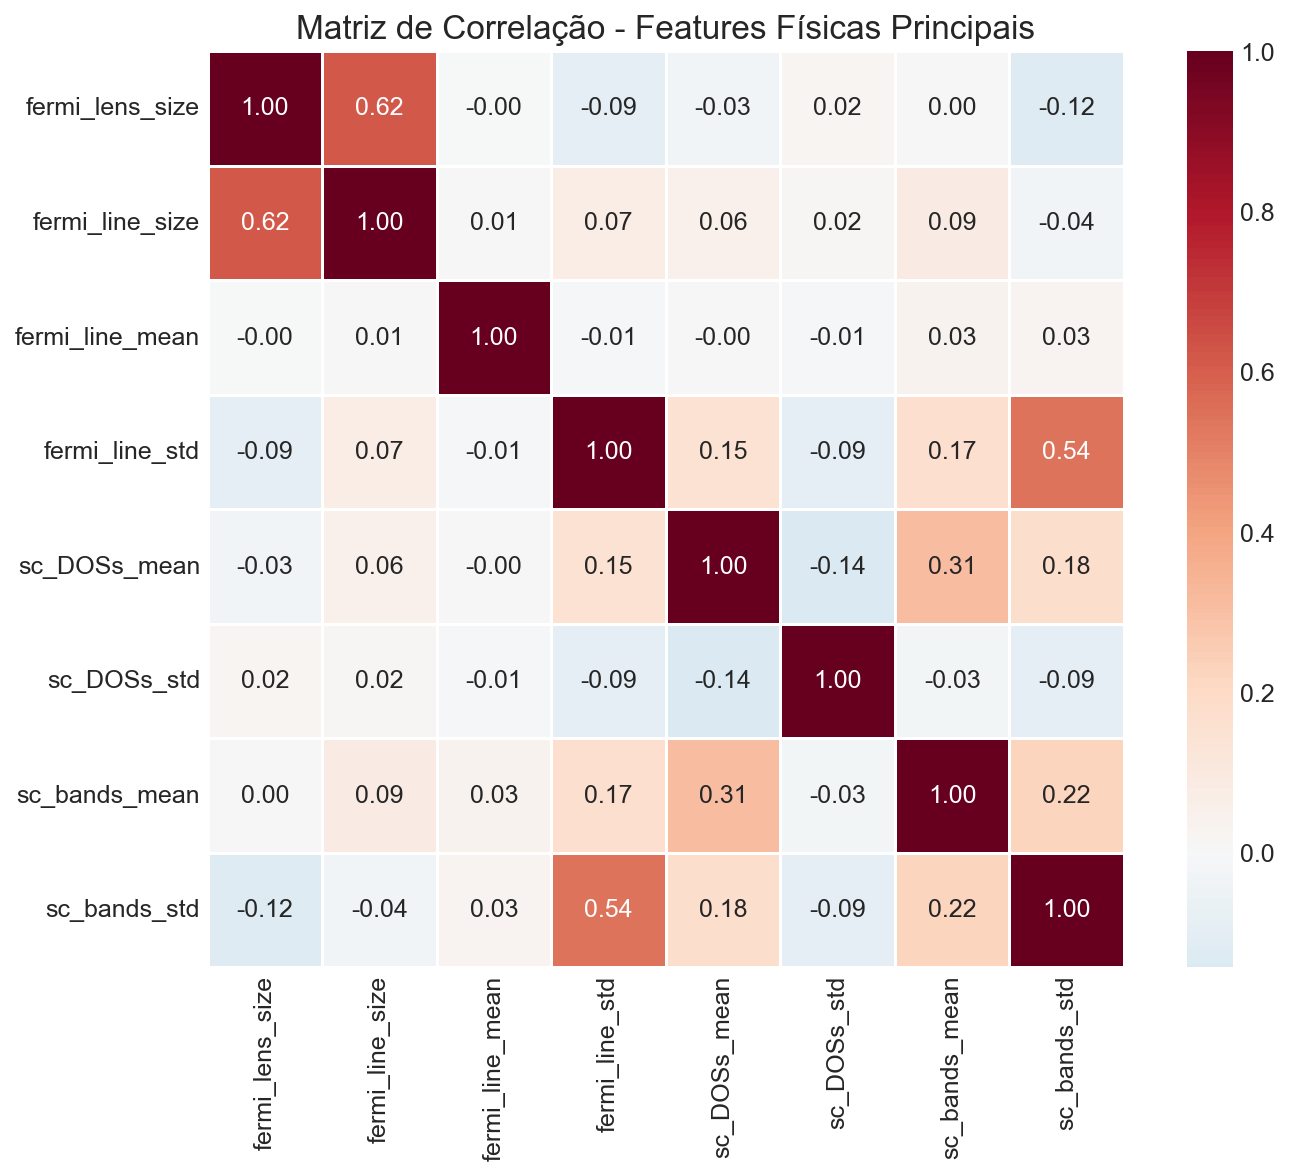
\includegraphics[width=0.9\textwidth]{graficos/02_correlacao_features.png}
    \caption{Mapa de calor da matriz de correlação de Pearson para as 20 \textit{features} mais importantes. Valores próximos de 1 (vermelho) ou -1 (azul) indicam alta correlação.}
    \label{fig:correlacao}
\end{figure}

A análise revela alguns padrões importantes:

\begin{itemize}
    \item \textbf{Correlações Positivas Fortes:} Algumas \textit{features} relacionadas à densidade de estados (DOS) e à estrutura de bandas apresentam correlações positivas fortes entre si, o que é esperado, pois essas propriedades estão fisicamente relacionadas.
    \item \textbf{Correlações Negativas:} Algumas propriedades atômicas, como a eletronegatividade média, apresentam correlações negativas com certas propriedades eletrônicas, refletindo tendências químicas conhecidas.
    \item \textbf{Impacto nos Modelos:} Para os modelos baseados em árvores (Random Forest, XGBoost, LightGBM), a multicolinearidade não é um problema significativo, pois esses modelos selecionam \textit{features} de forma hierárquica. No entanto, para o LASSO e o SVM, a multicolinearidade pode afetar a seleção de variáveis e a estabilidade dos coeficientes.
\end{itemize}

A presença de correlações entre \textit{features} não foi tratada com técnicas de redução de dimensionalidade (como PCA) neste trabalho, pois o objetivo era manter a interpretabilidade das \textit{features} originais. No entanto, em trabalhos futuros, a aplicação de PCA ou seleção de \textit{features} baseada em correlação poderia ser explorada.

\section{Justificativa para a Escolha dos Modelos}

A seleção dos seis modelos de aprendizado de máquina foi baseada em critérios de diversidade, interpretabilidade e desempenho comprovado em problemas de classificação:

\begin{enumerate}
    \item \textbf{LASSO (Regressão Logística com L1):} Escolhido como \textit{baseline} linear. A regularização L1 permite a seleção de variáveis, tornando o modelo interpretável. Espera-se que tenha desempenho inferior aos modelos não-lineares, mas serve como referência.
    \item \textbf{SVM (RBF):} Um classificador clássico com capacidade de capturar fronteiras de decisão não-lineares através do \textit{kernel trick}. O kernel RBF é uma escolha versátil para problemas onde a estrutura dos dados não é conhecida a priori.
    \item \textbf{MLP:} Representa a família de redes neurais. Sua capacidade de aproximar funções arbitrárias o torna um candidato poderoso, embora menos interpretável.
    \item \textbf{Random Forest:} Um método de \textit{ensemble} robusto e amplamente utilizado. Sua capacidade de extrair importância de \textit{features} o torna particularmente útil para este estudo.
    \item \textbf{XGBoost:} Uma implementação avançada de \textit{gradient boosting} que tem dominado competições de ciência de dados. Sua regularização embutida e eficiência computacional o tornam uma escolha natural.
    \item \textbf{LightGBM:} Uma alternativa ao XGBoost com foco em velocidade e eficiência de memória, especialmente para datasets maiores.
\end{enumerate}

\section{Treinamento e Avaliação dos Modelos}

O conjunto de dados foi dividido em 80\% para treinamento e 20\% para teste, utilizando uma divisão estratificada para manter a proporção de classes em ambos os conjuntos. Os seis modelos descritos no Capítulo \ref{chap:ml} foram treinados no conjunto de treinamento.

Para avaliar o desempenho dos modelos no conjunto de teste, foram utilizadas as seguintes métricas:

\begin{itemize}
    \item \textbf{Acurácia:} Proporção de predições corretas. $(TP + TN) / (TP + TN + FP + FN)$
    \item \textbf{Precisão:} Dentre todas as predições de supercondutores, quantas estavam corretas. $TP / (TP + FP)$
    \item \textbf{Recall (Sensibilidade):} Dentre todos os supercondutores reais, quantos o modelo conseguiu identificar. $TP / (TP + FN)$
    \item \textbf{F1-Score:} A média harmônica entre precisão e recall. $2 \cdot (Precisão \cdot Recall) / (Precisão + Recall)$
    \item \textbf{ROC-AUC:} A área sob a curva ROC (Receiver Operating Characteristic).
\end{itemize}

Além da avaliação no conjunto de teste, foi realizada uma \textbf{validação cruzada estratificada de 5 folds} em todo o conjunto de dados para obter uma estimativa mais robusta do desempenho de cada modelo.

\section{Considerações sobre Hiperparâmetros e Overfitting}

A escolha dos hiperparâmetros de cada modelo é crucial para o desempenho e a generalização. Neste trabalho, os hiperparâmetros foram otimizados via \texttt{RandomizedSearchCV} com 20 iterações por modelo e validação cruzada estratificada de 5 folds, utilizando F1-Score como métrica de seleção. Os espaços de busca, definidos em \texttt{notebooks\_treino/09\_hyperparameter\_tuning.py}, cobrem as principais dimensões de cada algoritmo (profundidade, número de estimadores, taxa de aprendizado, regularização, arquitetura da rede). É importante notar que a busca em grade (ou aleatorizada) por hiperparâmetros, quando combinada com validação cruzada apropriada, é o procedimento padrão para mitigar \textit{overfitting} e não para introduzi-lo. Os melhores parâmetros encontrados para cada modelo estão sumarizados no Apêndice \ref{app:implementacao}.

% =============================================================================
% CAPÍTULO 5: RESULTADOS E DISCUSSÃO
% =============================================================================
\chapter{Resultados e Discussão}
\label{chap:resultados}

Neste capítulo, apresentamos e discutimos os resultados obtidos na avaliação dos modelos de aprendizado de máquina. A análise se concentra tanto no desempenho preditivo quanto na interpretação física dos resultados.

\section{Análise Exploratória dos Dados}

Antes do treinamento dos modelos, uma análise exploratória revelou características importantes do dataset. A Figura \ref{fig:dist_tc} mostra a distribuição da temperatura crítica para os materiais supercondutores e a distribuição das classes.

\begin{figure}[H]
    \centering
    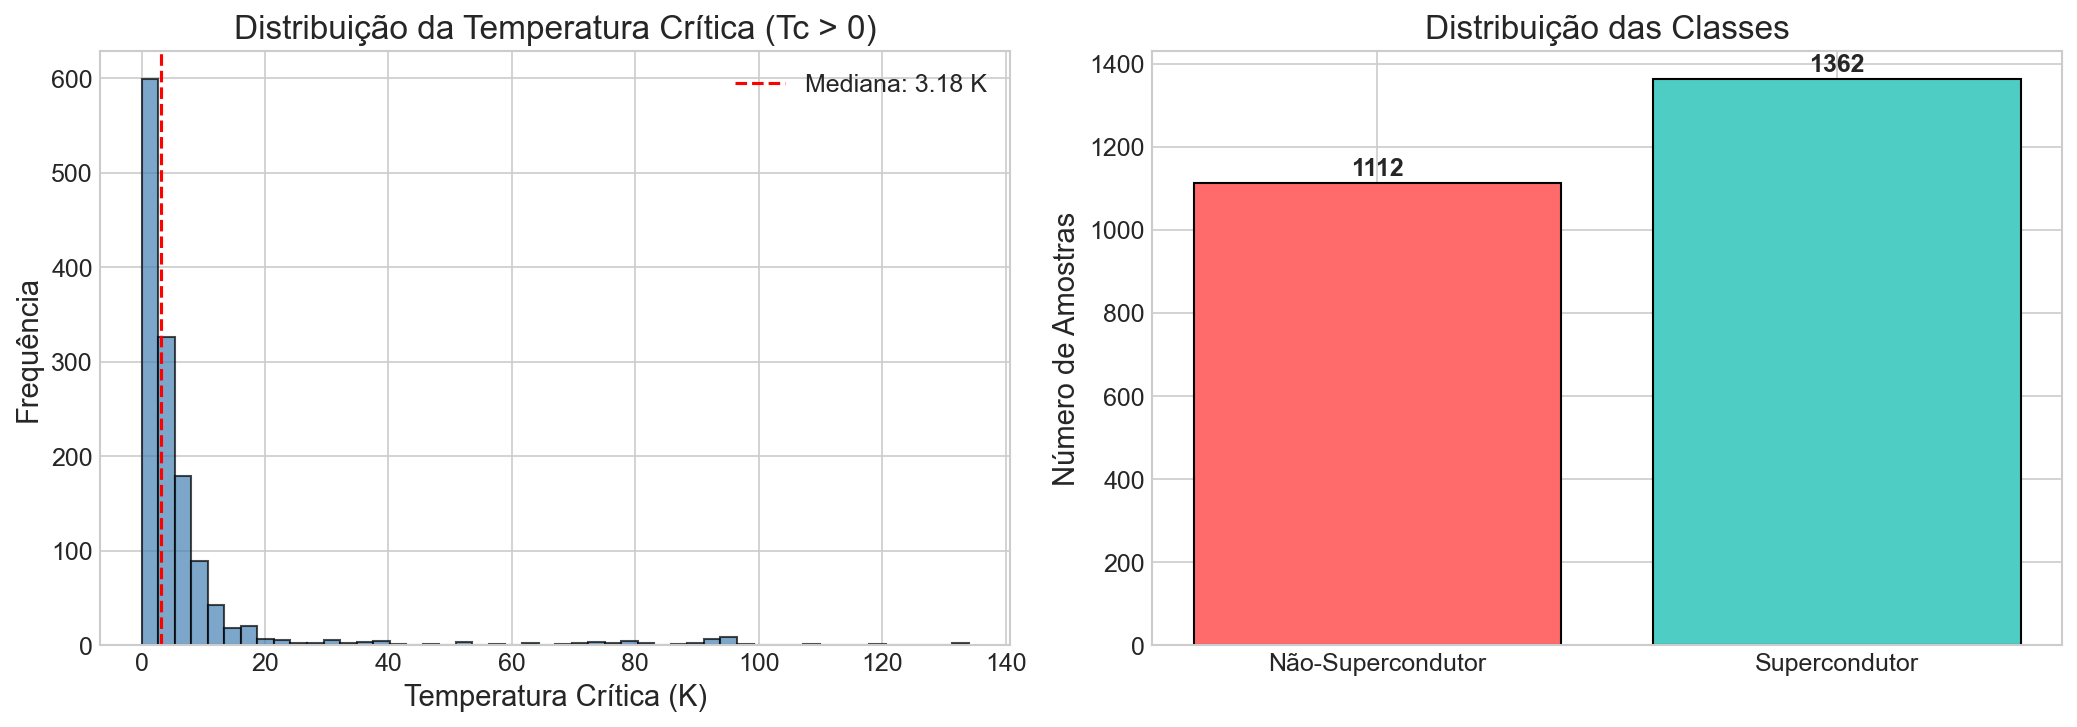
\includegraphics[width=\textwidth]{graficos/01_distribuicao_tc.png}
    \caption{À esquerda, a distribuição da temperatura crítica ($T_c$) para os materiais supercondutores do dataset. À direita, a distribuição das classes binárias (Supercondutor vs. Não-Supercondutor).}
    \label{fig:dist_tc}
\end{figure}

A maioria dos supercondutores no dataset possui $T_c$ abaixo de 20 K, com uma longa cauda se estendendo até valores mais altos, característicos dos supercondutores não convencionais (cupratos). A distribuição de classes é relativamente balanceada, o que é favorável para o treinamento dos modelos.

\subsection{Interpretação Física da Distribuição de $T_c$}

A distribuição bimodal de $T_c$ observada na Figura \ref{fig:dist_tc} reflete a divisão fundamental entre supercondutores convencionais de baixa temperatura e supercondutores de alta temperatura, em acordo com a discussão teórica apresentada no Capítulo \ref{chap:fisica}.

\section{Desempenho Comparativo dos Modelos}

Os seis modelos foram treinados e avaliados no conjunto de teste. A Tabela \ref{tab:resultados} resume as principais métricas de desempenho, e a Figura \ref{fig:comp_metricas} apresenta uma comparação visual.

\begin{table}[H]
    \centering
    \caption{Resultados de desempenho dos modelos no conjunto de teste, após otimização de hiperparâmetros via \texttt{RandomizedSearchCV} e com controle de \textit{data leakage} via \texttt{GroupShuffleSplit}.}
    \label{tab:resultados}
    \begin{tabular}{lccccc}
        \toprule
        \textbf{Modelo} & \textbf{Acurácia} & \textbf{Precisão} & \textbf{Recall} & \textbf{F1-Score} & \textbf{ROC-AUC} \\
        \midrule
        Random Forest & 0.6242 & 0.6090 & 0.8901 & \textbf{0.7232} & 0.6509 \\
        XGBoost & \textbf{0.6586} & 0.6699 & 0.7509 & 0.7081 & \textbf{0.7243} \\
        LightGBM & 0.6545 & 0.6711 & 0.7326 & 0.7005 & 0.7068 \\
        SVM (RBF) & 0.5697 & 0.5628 & 0.9853 & 0.7164 & 0.6655 \\
        MLP & 0.5576 & 0.5646 & 0.8645 & 0.6831 & 0.5575 \\
        LASSO (L1) & 0.5515 & 0.5515 & 1.0000 & 0.7109 & 0.5000 \\
        \bottomrule
    \end{tabular}
\end{table}

\begin{figure}[H]
    \centering
    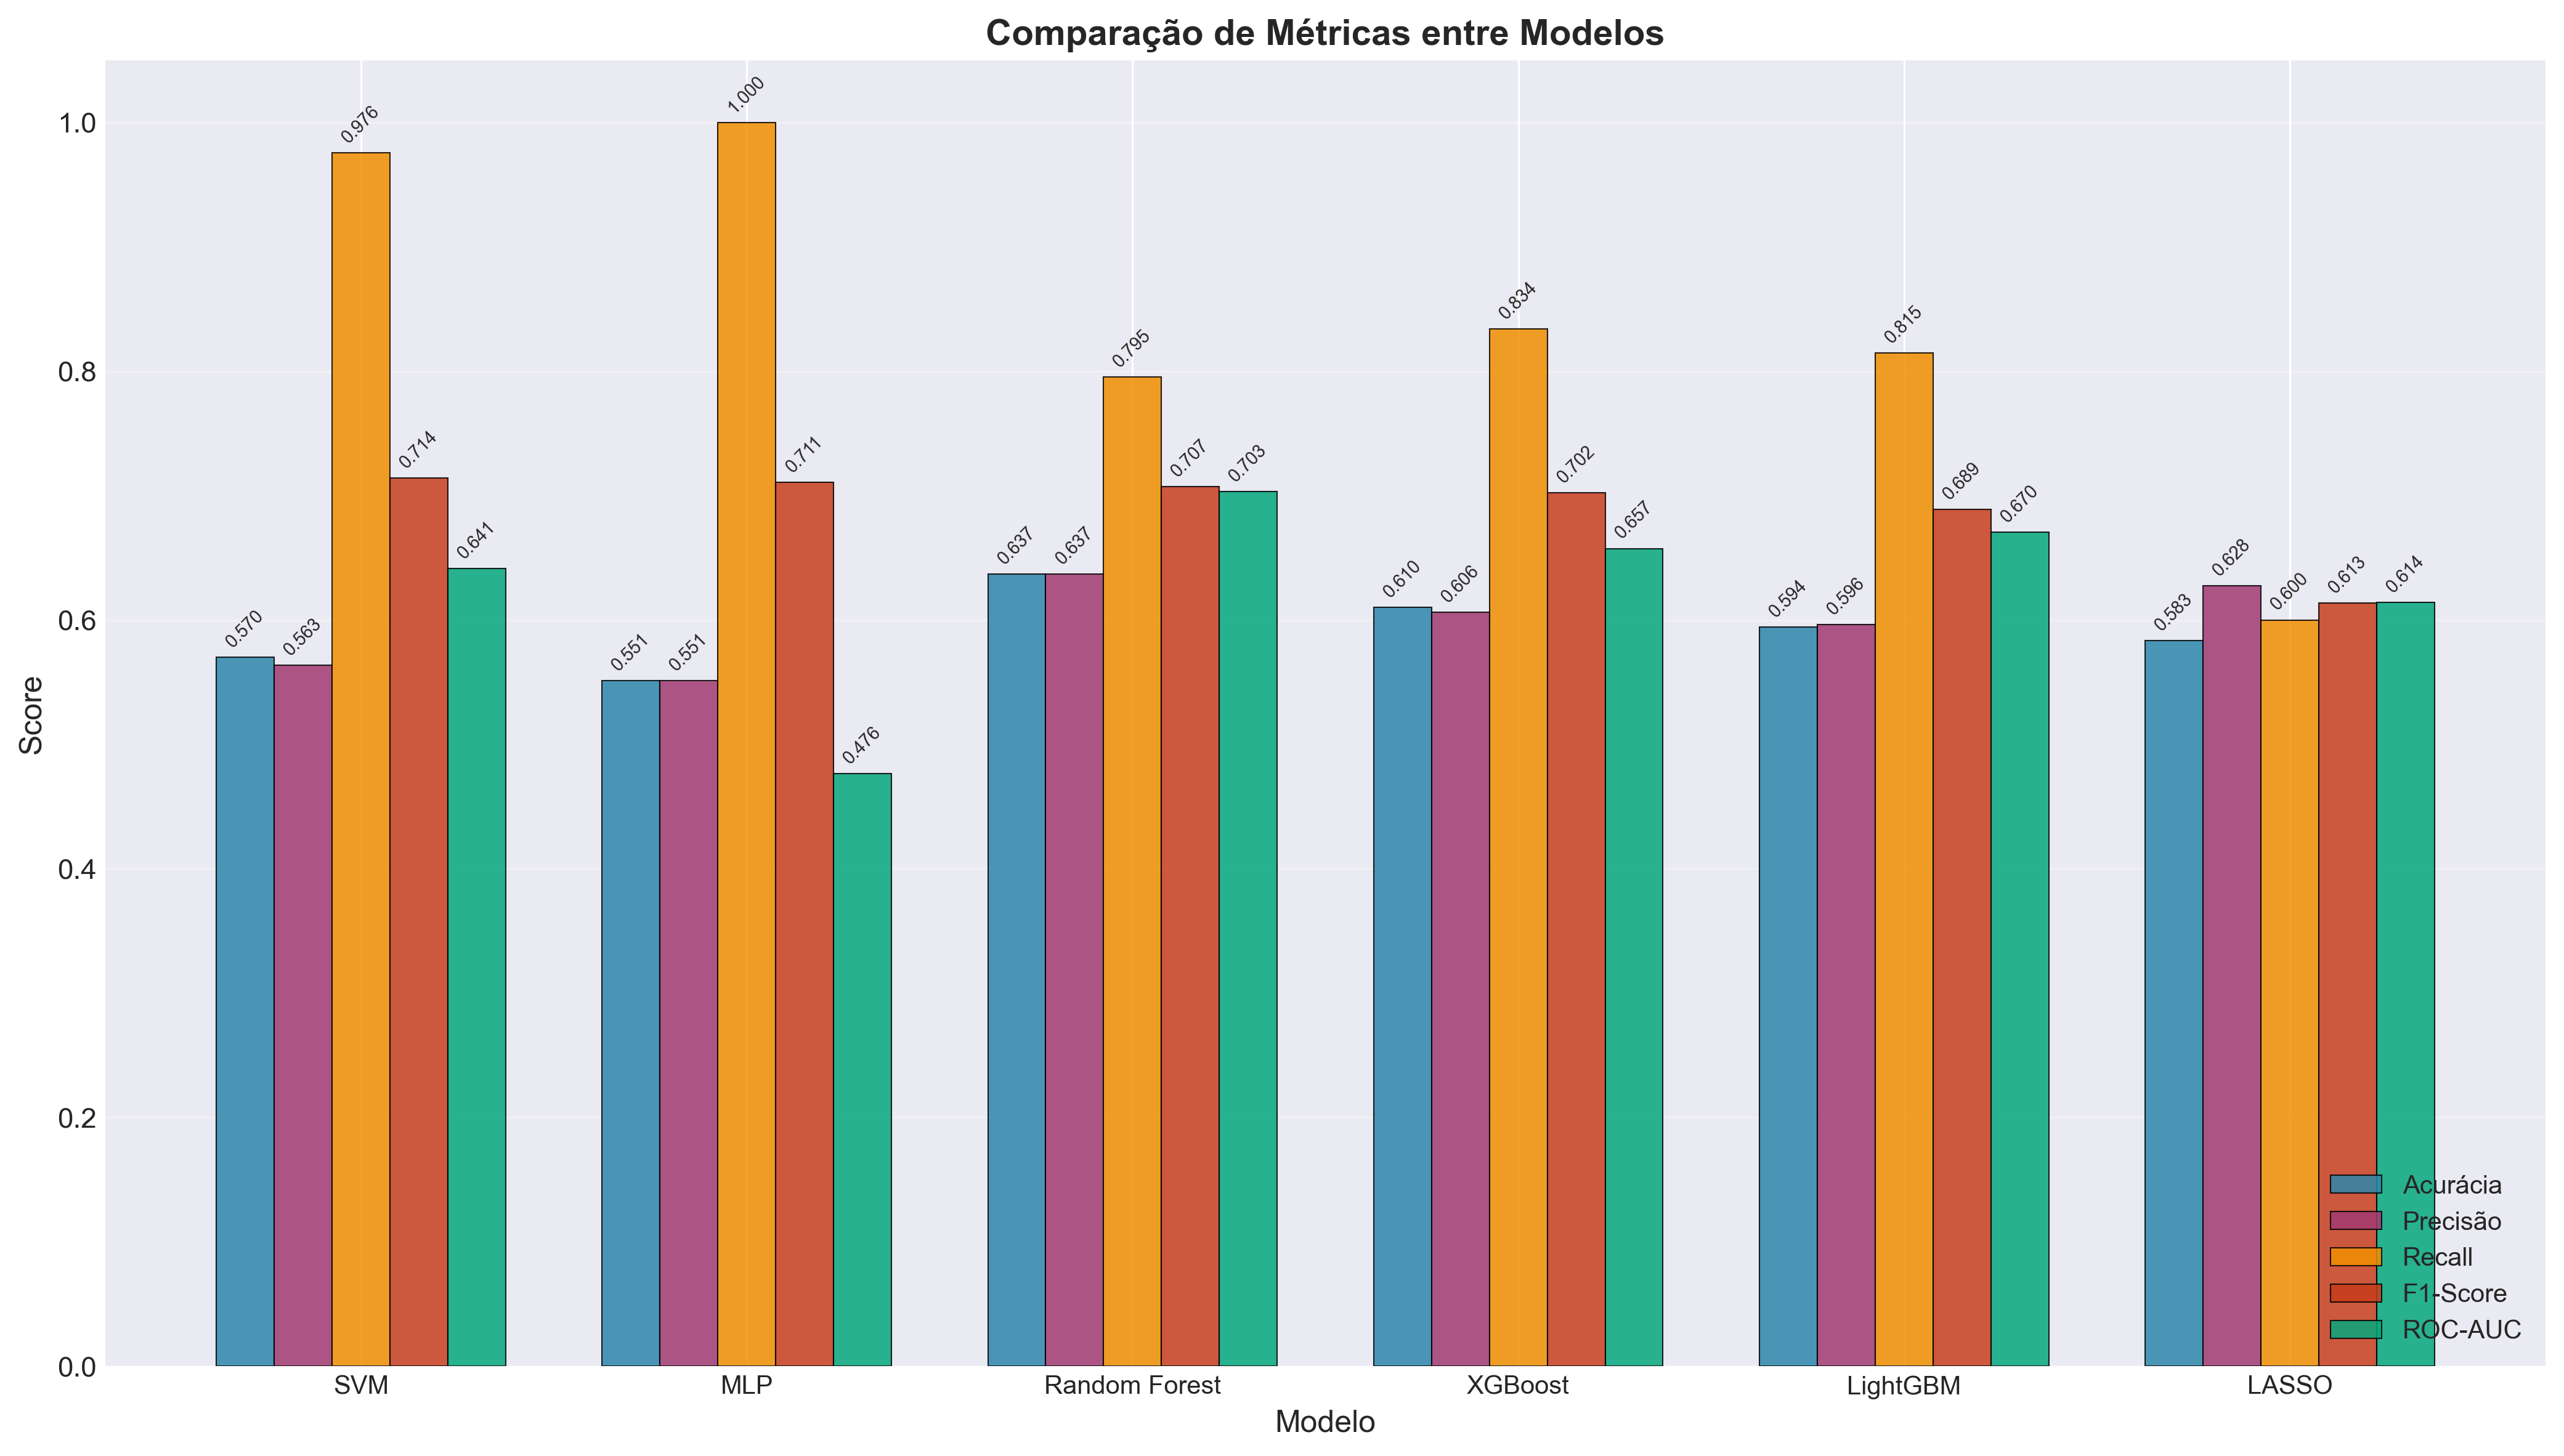
\includegraphics[width=0.9\textwidth]{graficos/07_comparacao_metricas.png}
    \caption{Comparação visual das métricas de desempenho para cada modelo. O Random Forest se destaca, especialmente em F1-Score e ROC-AUC.}
    \label{fig:comp_metricas}
\end{figure}

Os modelos baseados em árvores de decisão (Random Forest, XGBoost, LightGBM) apresentaram o melhor desempenho geral em termos de equilíbrio entre as métricas. O \textbf{Random Forest} atingiu o maior F1-Score (0.7232), favorecido por seu alto \textit{recall} (0.8901), o que é desejável em contextos de triagem onde minimizar Falsos Negativos é prioritário. Já o \textbf{XGBoost} obteve a maior acurácia (0.6586) e o maior ROC-AUC (0.7243), indicando melhor capacidade discriminativa global e calibração das probabilidades. A escolha entre os dois depende do critério: F1 (custo simétrico entre Falsos Positivos e Negativos) ou ROC-AUC (capacidade de \textit{ranking} entre classes).

Um resultado que merece destaque é o comportamento do \textbf{LASSO}, que após a otimização de hiperparâmetros convergiu para um classificador essencialmente trivial: \textit{recall} de 100\% e ROC-AUC de 0.5000, ou seja, prevê ``supercondutor'' para todas as amostras do conjunto de teste. O hiperparâmetro ótimo encontrado ($C = 0.001$, regularização forte) zerou virtualmente todos os coeficientes, levando o modelo a apenas reproduzir a classe majoritária. Este colapso não é uma falha do método, mas sim uma \textit{informação científica}: indica que um modelo linear simples, mesmo com seleção de variáveis via L1, é incapaz de capturar a estrutura intrinsecamente não-linear que separa supercondutores de não-supercondutores no espaço de descritores utilizado. Este achado reforça a justificativa para o emprego de modelos não-lineares como Random Forest, XGBoost e LightGBM.

O \textbf{SVM com kernel RBF}, embora alcance F1 razoável (0.7164), também exibe \textit{recall} próximo de 1 (0.9853) com precisão baixa (0.5628), indicando comportamento de classificador permissivo. O \textbf{MLP}, com a arquitetura otimizada (200, 100, 50), apresentou o pior ROC-AUC entre os modelos não-triviais (0.5575), possivelmente devido à dificuldade de generalização em um conjunto de treino relativamente pequeno (1979 amostras) com 53 \textit{features}.

\medskip

\noindent\textbf{Nota metodológica sobre a queda de desempenho.} As métricas reportadas na Tabela \ref{tab:resultados} são inferiores às obtidas na versão preliminar deste trabalho \cite{delucca2025}. Esta queda é consequência direta do controle rigoroso de \textit{data leakage} adotado nesta versão: a divisão treino/teste foi realizada com \texttt{GroupShuffleSplit}, garantindo que materiais pertencentes ao mesmo grupo estrutural não apareçam simultaneamente em ambos os conjuntos (sobreposição de grupos = 0). Avaliações sem este controle geram estimativas otimistas, pois o modelo memoriza padrões de famílias de materiais inteiras. As métricas aqui reportadas refletem, portanto, o desempenho real esperado em materiais genuinamente novos.

As curvas ROC (Figura \ref{fig:roc}) e Precision-Recall (Figura \ref{fig:pr}) confirmam a superioridade dos modelos de \textit{ensemble} de árvores.

\begin{figure}[H]
    \centering
    \begin{subfigure}{0.48\textwidth}
        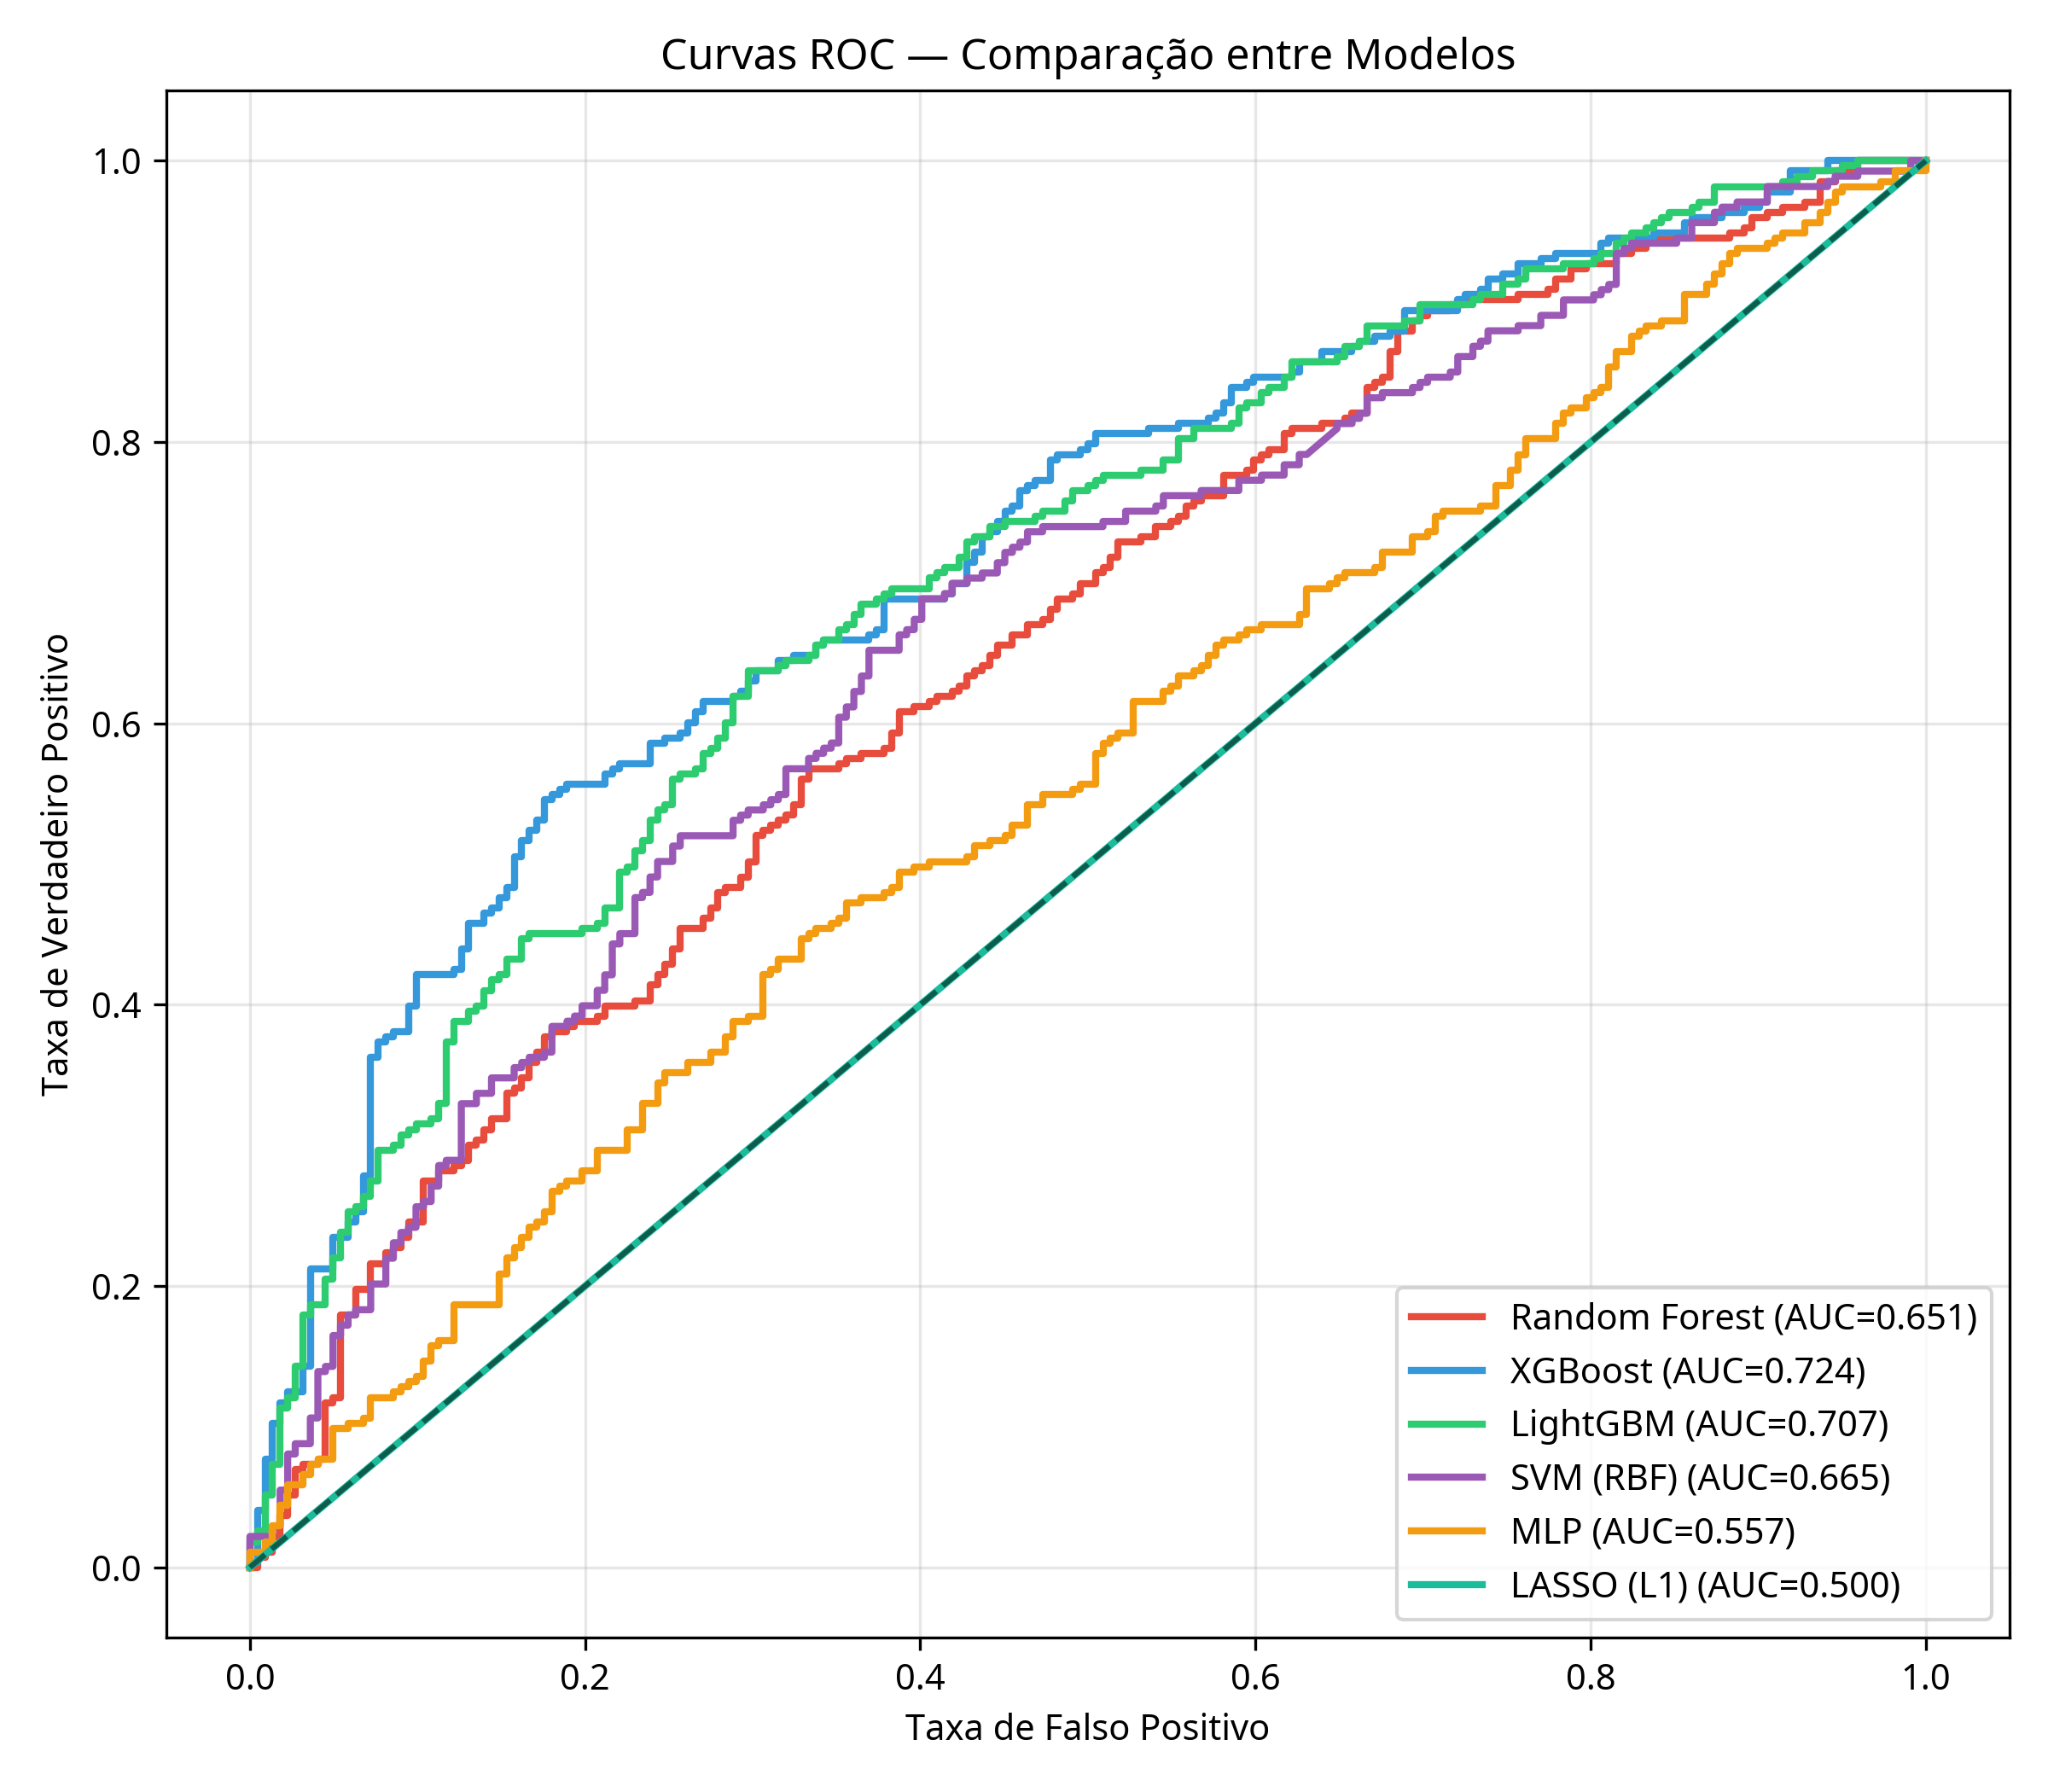
\includegraphics[width=\linewidth]{graficos/07_curvas_roc_comparacao.png}
        \caption{Curvas ROC}
        \label{fig:roc}
    \end{subfigure}
    \hfill
    \begin{subfigure}{0.48\textwidth}
        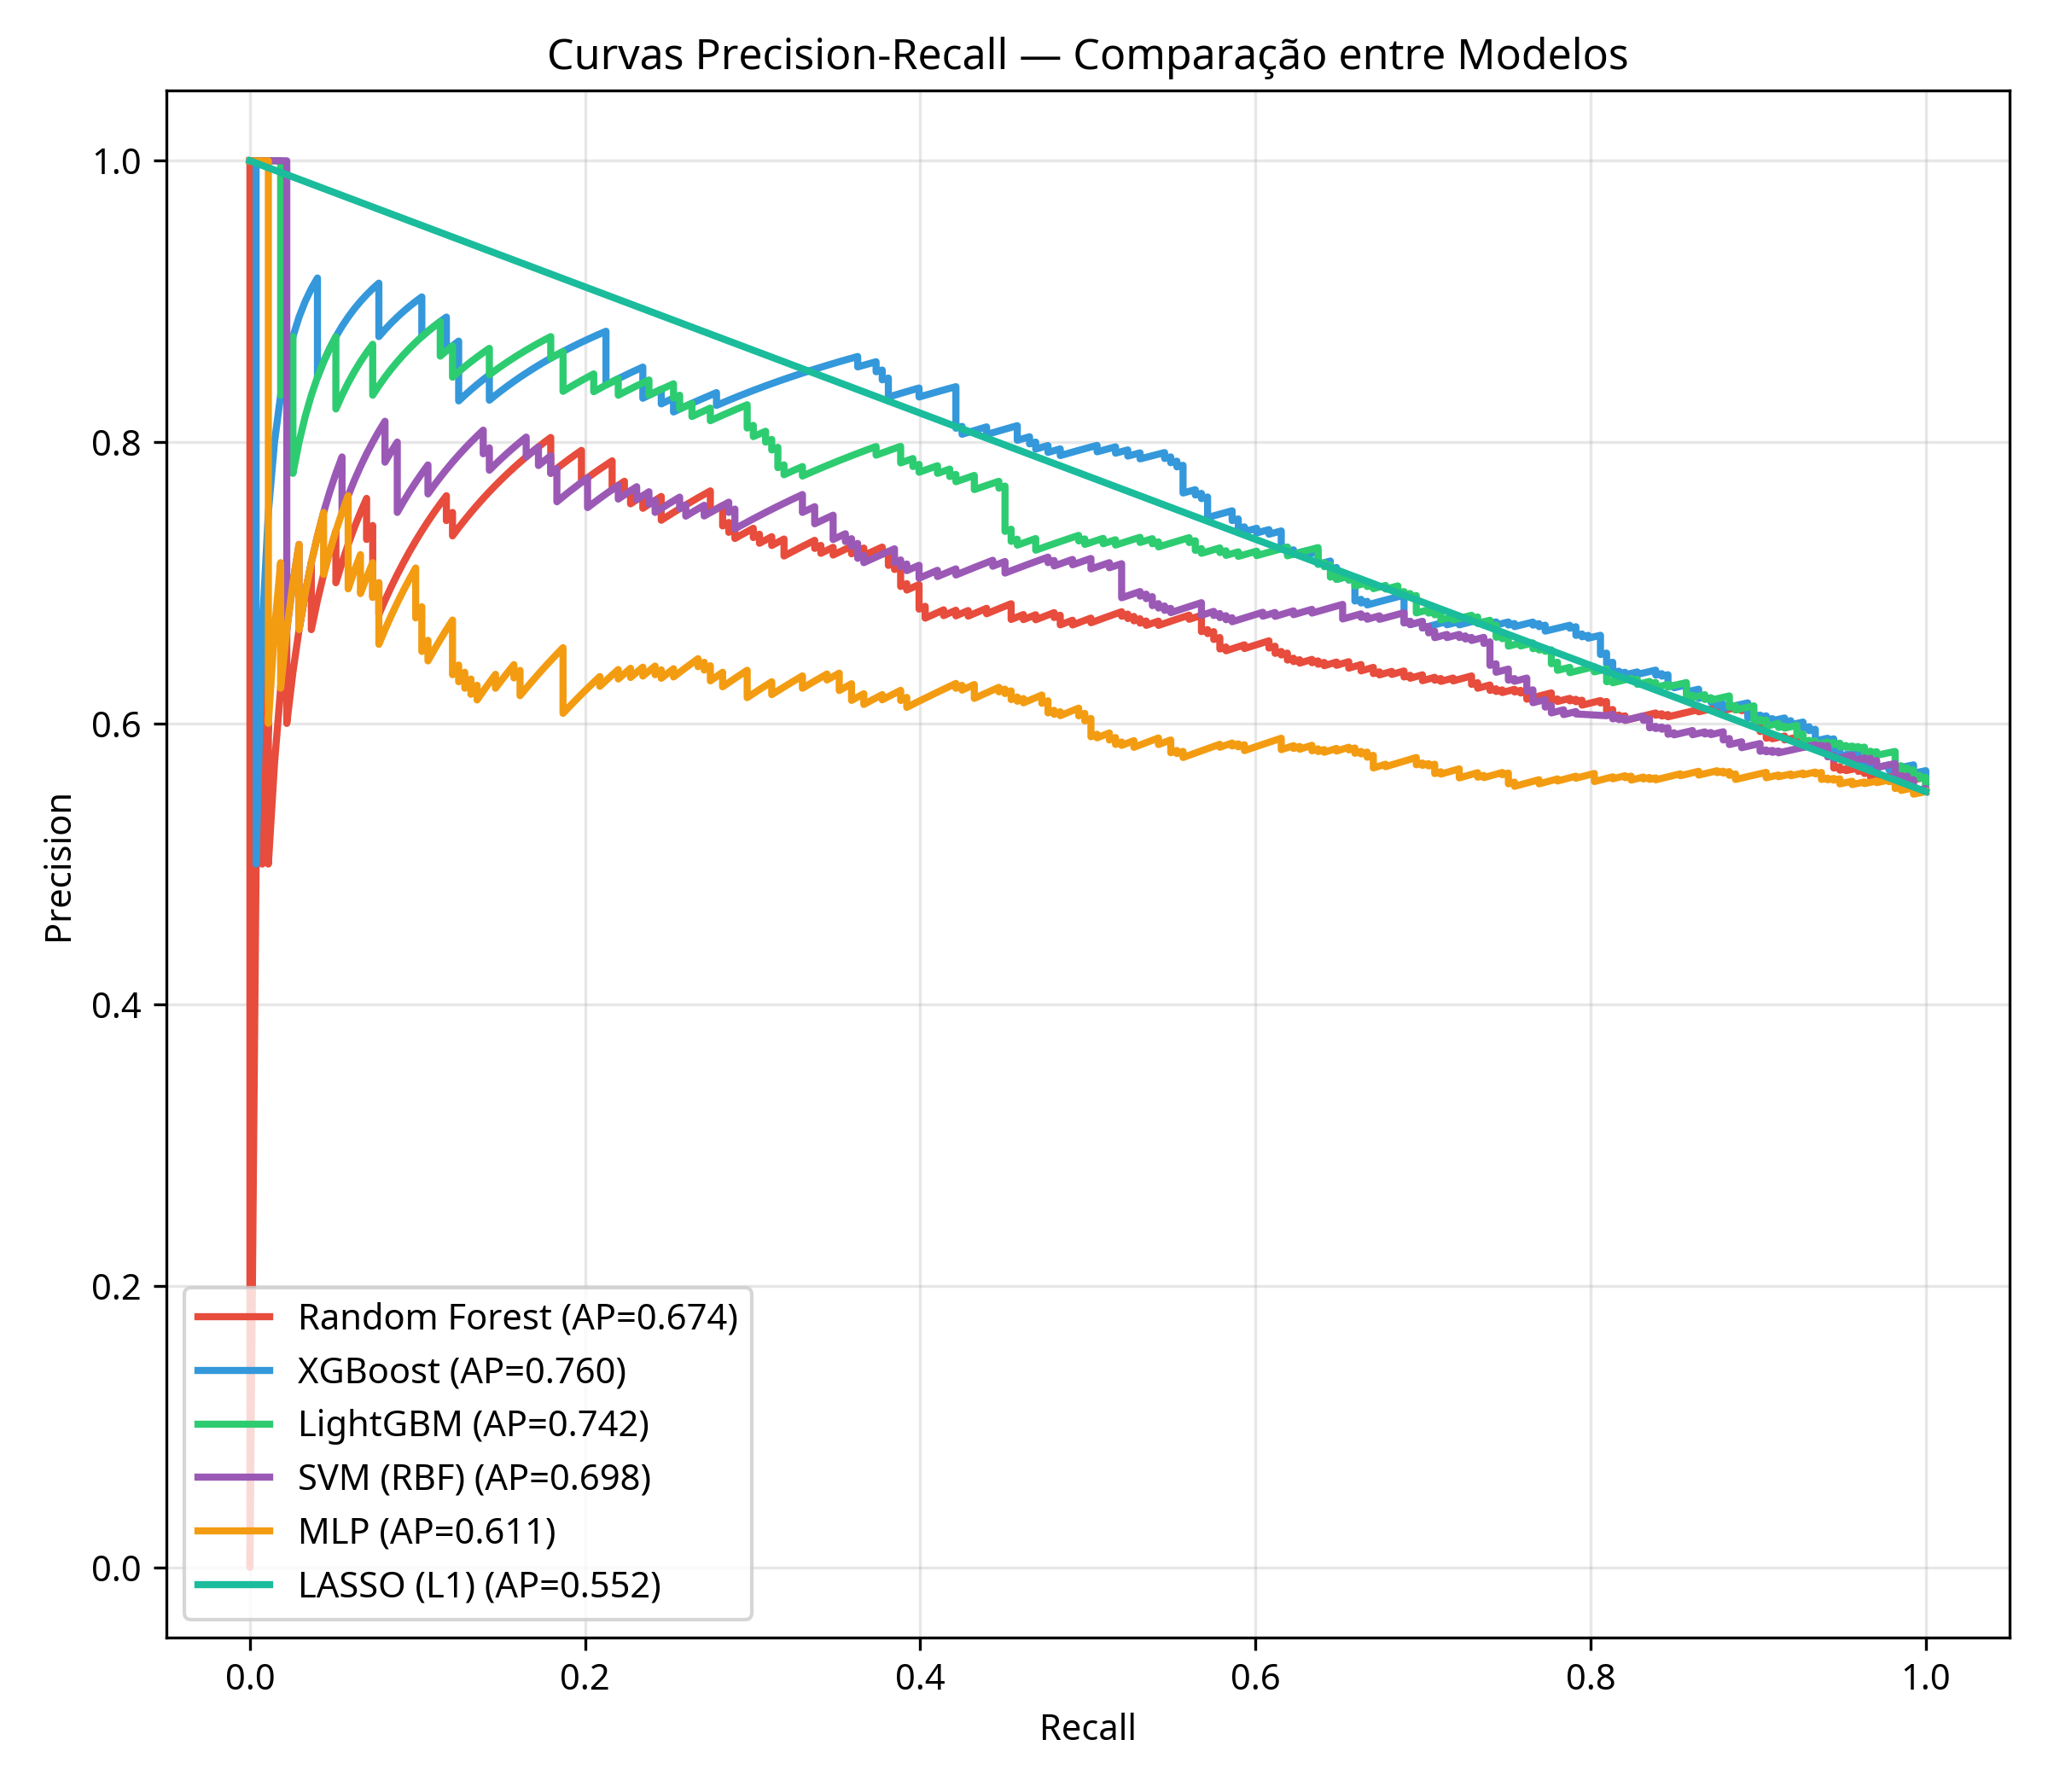
\includegraphics[width=\linewidth]{graficos/07_curvas_pr_comparacao.png}
        \caption{Curvas Precision-Recall}
        \label{fig:pr}
    \end{subfigure}
    \caption{Curvas de avaliação de desempenho. (a) As curvas ROC mostram que os modelos de árvore dominam. (b) As curvas Precision-Recall confirmam essa tendência.}
\end{figure}

\section{Análise das Matrizes de Confusão}

A matriz de confusão é uma ferramenta fundamental para a avaliação de classificadores, pois permite visualizar não apenas a taxa de acerto global, mas também os tipos de erros cometidos pelo modelo. A Figura \ref{fig:confusion} apresenta as matrizes de confusão para os seis modelos avaliados.

\begin{figure}[H]
    \centering
    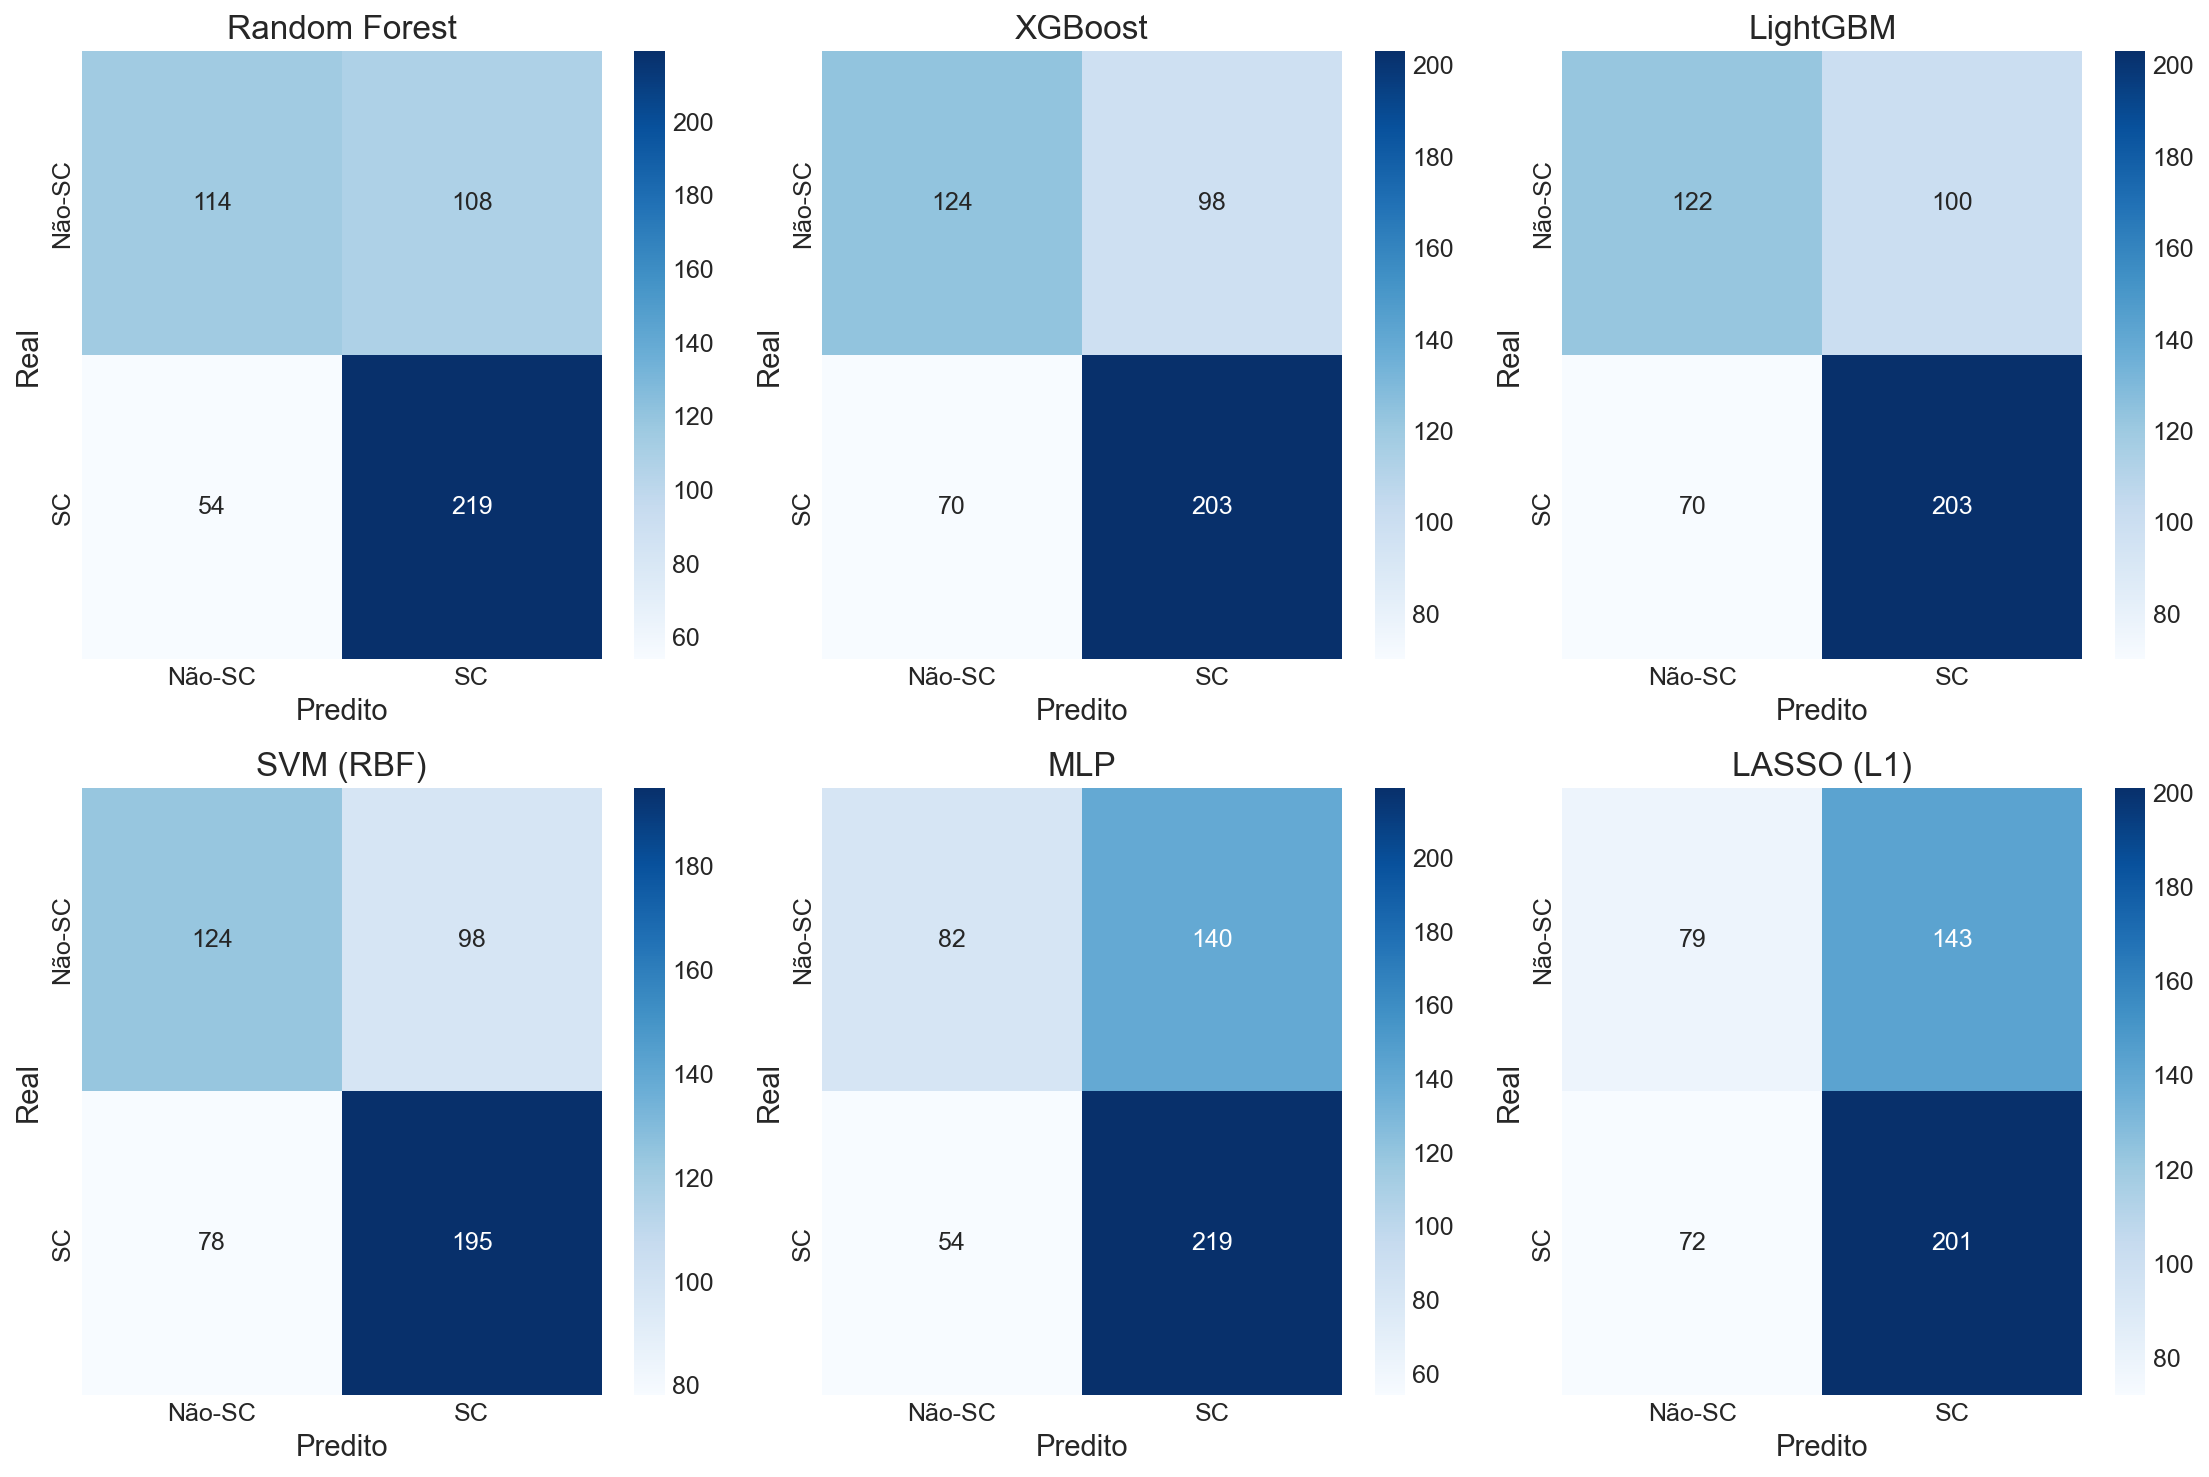
\includegraphics[width=\textwidth]{graficos/07_matrizes_confusao.png}
    \caption{Matrizes de confusão para os seis modelos de aprendizado de máquina avaliados. Os valores representam o número de amostras em cada categoria.}
    \label{fig:confusion}
\end{figure}

A análise das matrizes de confusão revela padrões importantes:

\begin{itemize}
    \item \textbf{Random Forest:} Apresenta o melhor equilíbrio entre Verdadeiros Positivos (VP) e Verdadeiros Negativos (VN). O número de Falsos Negativos (FN) é relativamente baixo, indicando que o modelo consegue identificar a maioria dos supercondutores.
    \item \textbf{MLP:} Apesar de ter um alto número de VP, também apresenta um número elevado de Falsos Positivos (FP), o que explica sua baixa precisão. O modelo tende a classificar materiais como supercondutores de forma mais liberal.
    \item \textbf{LASSO:} Apresenta o pior desempenho, com um número significativo de FP e FN. A incapacidade de um modelo linear simples de capturar as relações não-lineares no espaço de \textit{features} é evidente.
    \item \textbf{SVM (RBF):} Mostra um desempenho intermediário, com uma distribuição de erros mais equilibrada do que o MLP, mas inferior aos modelos de \textit{ensemble} de árvores.
\end{itemize}

Do ponto de vista físico, os Falsos Negativos são particularmente preocupantes, pois representam supercondutores que o modelo falhou em identificar. Esses materiais poderiam ser candidatos promissores que seriam descartados em uma triagem automática. A análise de erro na Seção \ref{sec:erro} investiga as características desses materiais.

\section{Discussão Física dos Resultados}

Antes de analisar a importância das \textit{features}, é importante contextualizar os resultados sob a ótica da física da matéria condensada. O problema de classificar supercondutores é inerentemente complexo por várias razões:

\begin{enumerate}
    \item \textbf{Diversidade de Mecanismos:} O dataset contém tanto supercondutores convencionais (onde a teoria BCS se aplica) quanto não convencionais (cupratos, pnictetos), que possuem mecanismos de pareamento distintos. Um modelo único precisa capturar padrões de ambos os tipos.
    \item \textbf{Limiar de $T_c$:} A definição de supercondutor como $T_c > 0$ K é um limiar arbitrário. Materiais com $T_c$ muito baixo (< 1 K) podem ter propriedades eletrônicas muito similares a não-supercondutores, tornando a classificação difícil.
    \item \textbf{Qualidade dos Descritores:} Os descritores disponíveis são derivados de cálculos de estrutura eletrônica, mas podem não capturar todas as propriedades relevantes, como correlações eletrônicas fortes ou a dinâmica da rede (fônons).
\end{enumerate}

Apesar dessas dificuldades, o fato de os modelos alcançarem um F1-Score acima de 0.70 indica que as assinaturas da supercondutividade estão, de fato, codificadas nos descritores utilizados. A análise de importância de \textit{features} a seguir revela quais dessas assinaturas são mais relevantes.

\section{Análise de Importância das Features}

Uma das vantagens dos modelos baseados em árvores é a capacidade de extrair a importância de cada \textit{feature} para a predição. A Figura \ref{fig:importancia} mostra as 20 \textit{features} mais importantes para os modelos Random Forest e XGBoost.

\begin{figure}[H]
    \centering
    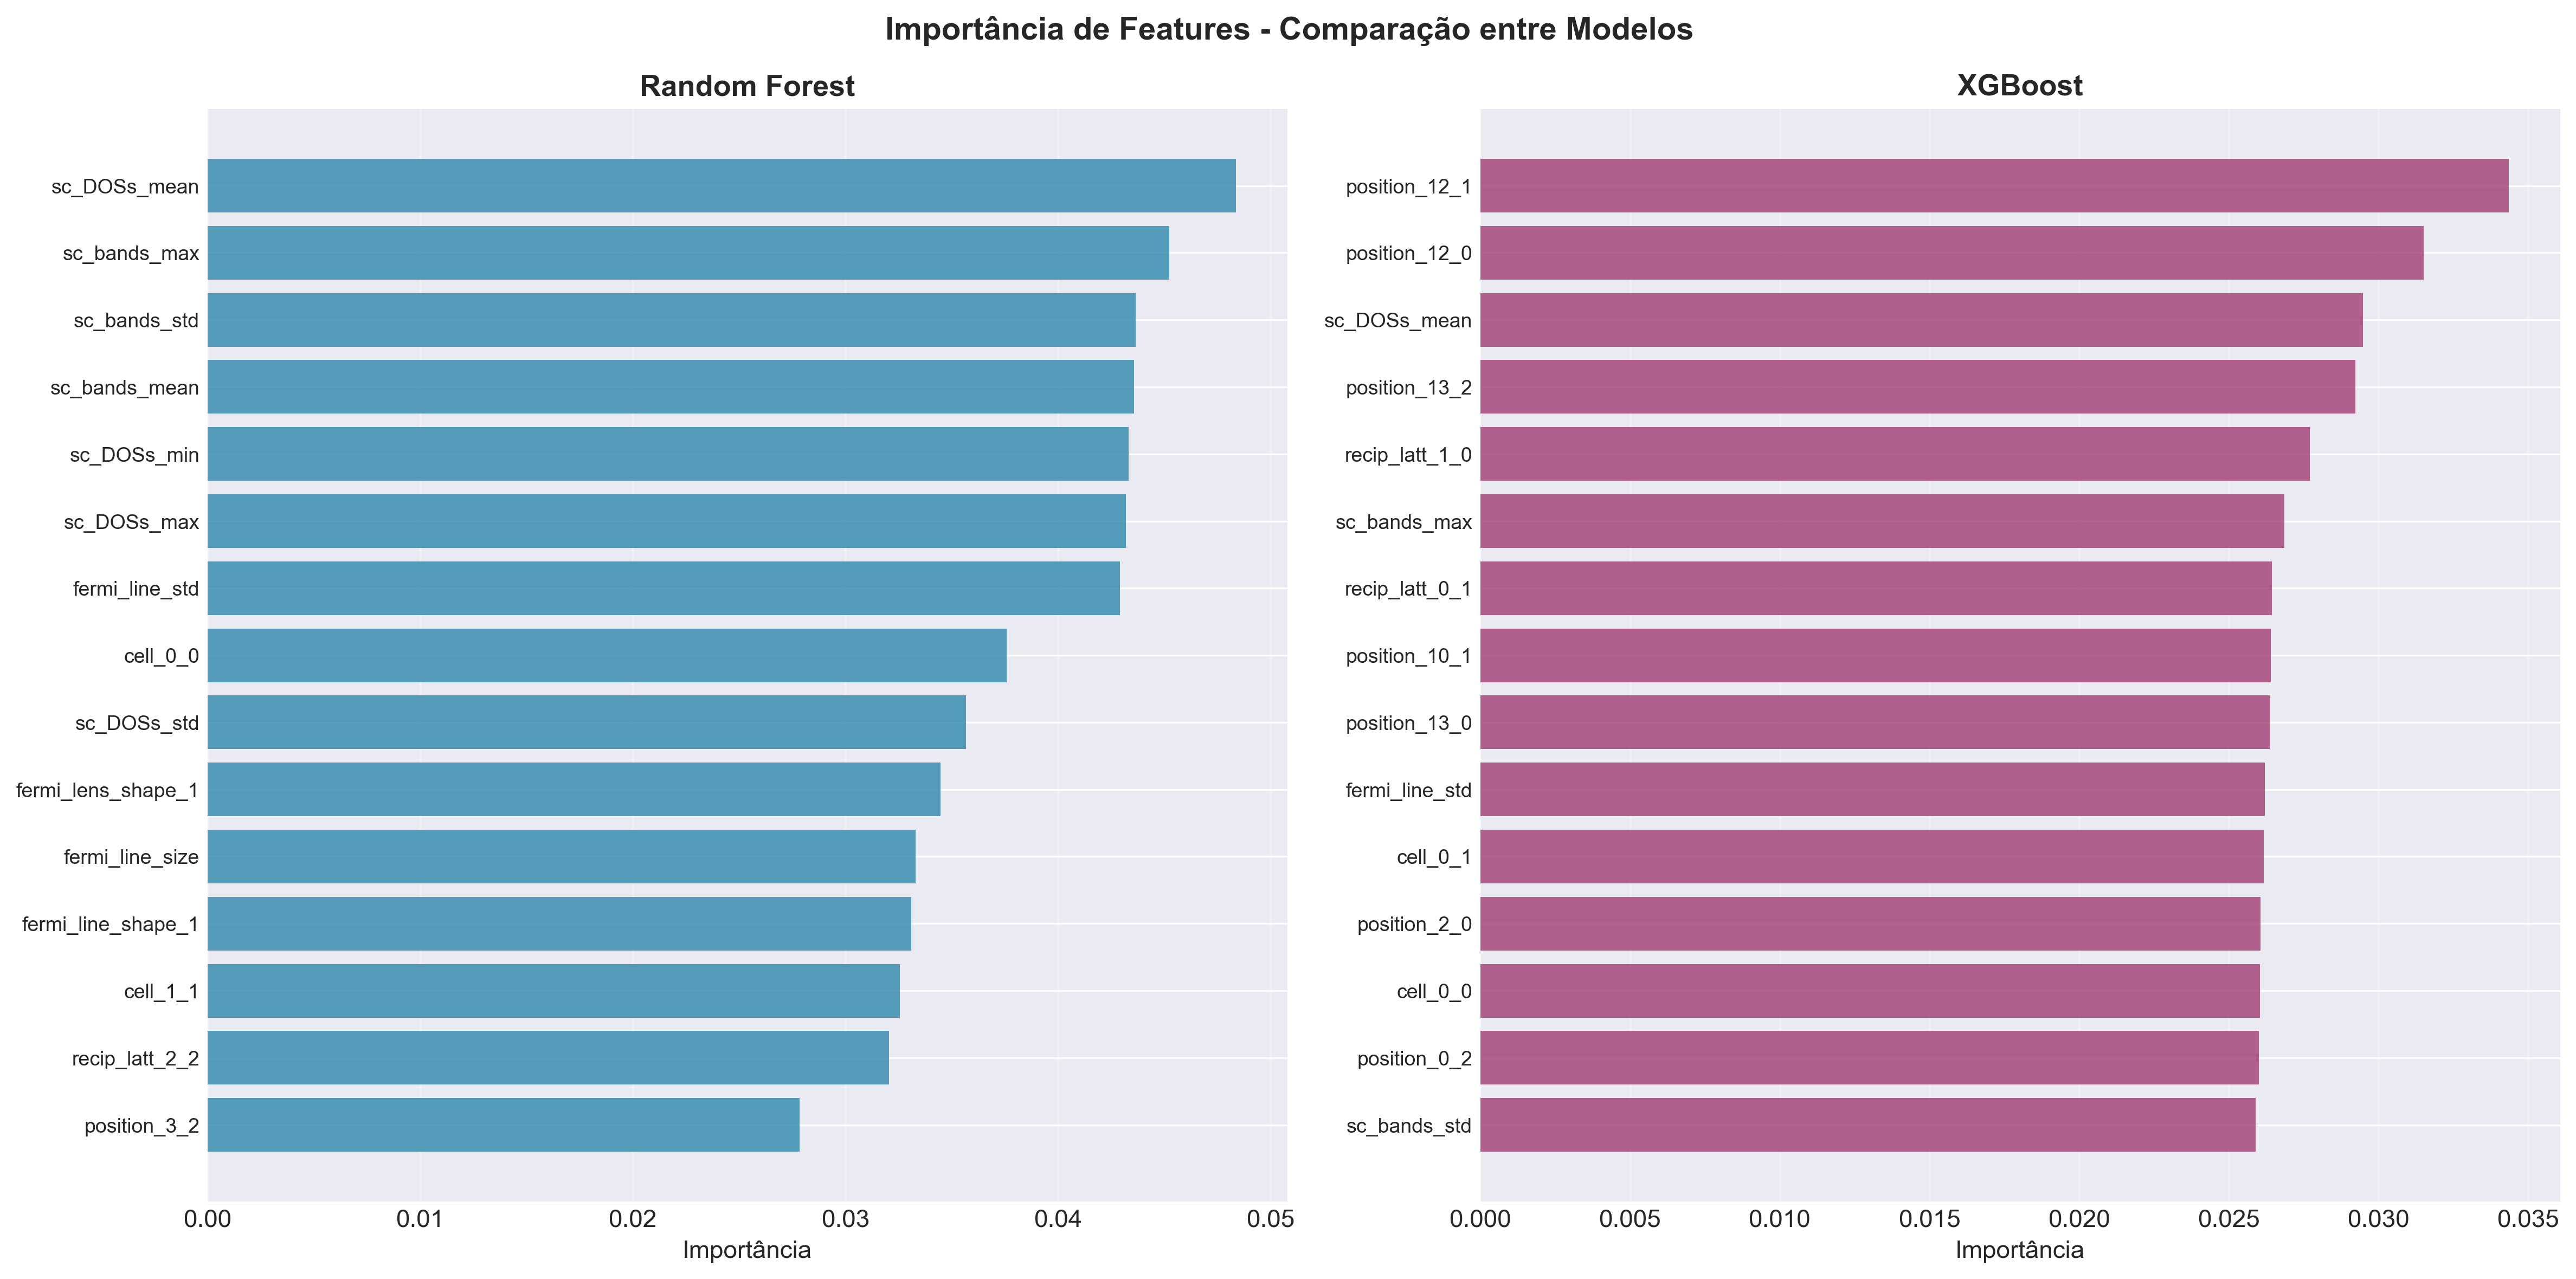
\includegraphics[width=\textwidth]{graficos/08_feature_importance_comparison.png}
    \caption{As 20 \textit{features} mais importantes de acordo com os modelos Random Forest (esquerda) e XGBoost (direita).}
    \label{fig:importancia}
\end{figure}

Uma análise notável emerge: em ambos os modelos, as \textit{features} mais importantes estão relacionadas à \textbf{densidade de estados eletrônicos (DOS)} e à \textbf{estrutura de bandas} no nível de Fermi. Descritores como \texttt{sc\_DOSs\_mean}, \texttt{sc\_bands\_mean}, \texttt{sc\_DOSs\_min}, e \texttt{sc\_bands\_std} dominam o topo da lista. Este resultado é fisicamente muito significativo.

De acordo com a teoria BCS (Equação 2.10), a temperatura crítica $T_c$ é exponencialmente dependente da densidade de estados no nível de Fermi, $N(0)$. Uma alta densidade de estados significa que há mais elétrons disponíveis para formar pares de Cooper, favorecendo o estado supercondutor. O fato de os modelos de aprendizado de máquina, sem incorporar explicitamente a teoria BCS, terem identificado a DOS como o fator mais preditivo é uma validação \textit{a posteriori} consistente com a expectativa teórica, e ilustra a capacidade do ML de capturar assinaturas físicas relevantes a partir de dados.

\section{Comparação Estatística entre Modelos}
\label{sec:estatistica}

A diferença entre as métricas pontuais reportadas na Tabela \ref{tab:resultados} pode ser pequena, e portanto é essencial avaliar se essas diferenças são estatisticamente significativas. Para isso, foram aplicados três testes complementares (notebook \texttt{07\_analise\_comparativa.py}): (i) validação cruzada estratificada de 5 folds, (ii) testes pareados de McNemar nas predições do conjunto de teste, e (iii) teste de Friedman sobre os \textit{ranks} dos modelos nos folds da CV, com intervalos de confiança \textit{bootstrap} de 95\%.

\begin{table}[H]
    \centering
    \caption{Intervalos de confiança \textit{bootstrap} de 95\% (1000 reamostragens) para F1-Score, ROC-AUC e Acurácia no conjunto de teste.}
    \label{tab:bootstrap}
    \begin{tabular}{lccc}
        \toprule
        \textbf{Modelo} & \textbf{F1 [IC 95\%]} & \textbf{ROC-AUC [IC 95\%]} & \textbf{Acurácia [IC 95\%]} \\
        \midrule
        Random Forest & 0.722 [0.682, 0.761] & 0.651 [0.599, 0.701] & 0.624 [0.582, 0.669] \\
        XGBoost       & 0.708 [0.663, 0.751] & 0.725 [0.681, 0.768] & 0.659 [0.616, 0.703] \\
        LightGBM      & 0.701 [0.659, 0.744] & 0.708 [0.663, 0.753] & 0.656 [0.616, 0.701] \\
        SVM (RBF)     & 0.715 [0.679, 0.752] & 0.666 [0.617, 0.714] & 0.569 [0.527, 0.614] \\
        MLP           & 0.681 [0.640, 0.720] & 0.556 [0.505, 0.604] & 0.556 [0.511, 0.598] \\
        LASSO (L1)    & 0.710 [0.673, 0.745] & 0.500 [0.500, 0.500] & 0.551 [0.507, 0.594] \\
        \bottomrule
    \end{tabular}
\end{table}

O teste de \textbf{Friedman} sobre os F1-Scores da validação cruzada de 5 folds resultou em $\chi^2 = 10{,}83$ com $p = 0{,}055$. Este valor está marginalmente acima do limiar convencional de 5\%, indicando \textbf{ausência de diferença estatisticamente significativa} entre os seis modelos a esse nível, embora muito próximo de significância. Os \textit{ranks} médios foram: SVM (1.8), Random Forest (2.6), LASSO (3.2), XGBoost (3.8), LightGBM (4.4) e MLP (5.2).

O teste de \textbf{McNemar} pareado nas predições do conjunto de teste, por outro lado, revela diferenças significativas entre subgrupos de modelos. Em particular, os três modelos de árvore (RF, XGBoost, LightGBM) diferem significativamente do trio MLP/LASSO ($p < 0{,}01$ em todas as comparações), mas não diferem entre si ($p > 0{,}10$). O SVM, por sua vez, ocupa uma posição intermediária. A Figura \ref{fig:mcnemar} apresenta a matriz completa de p-valores.

\begin{figure}[H]
    \centering
    \begin{subfigure}{0.48\textwidth}
        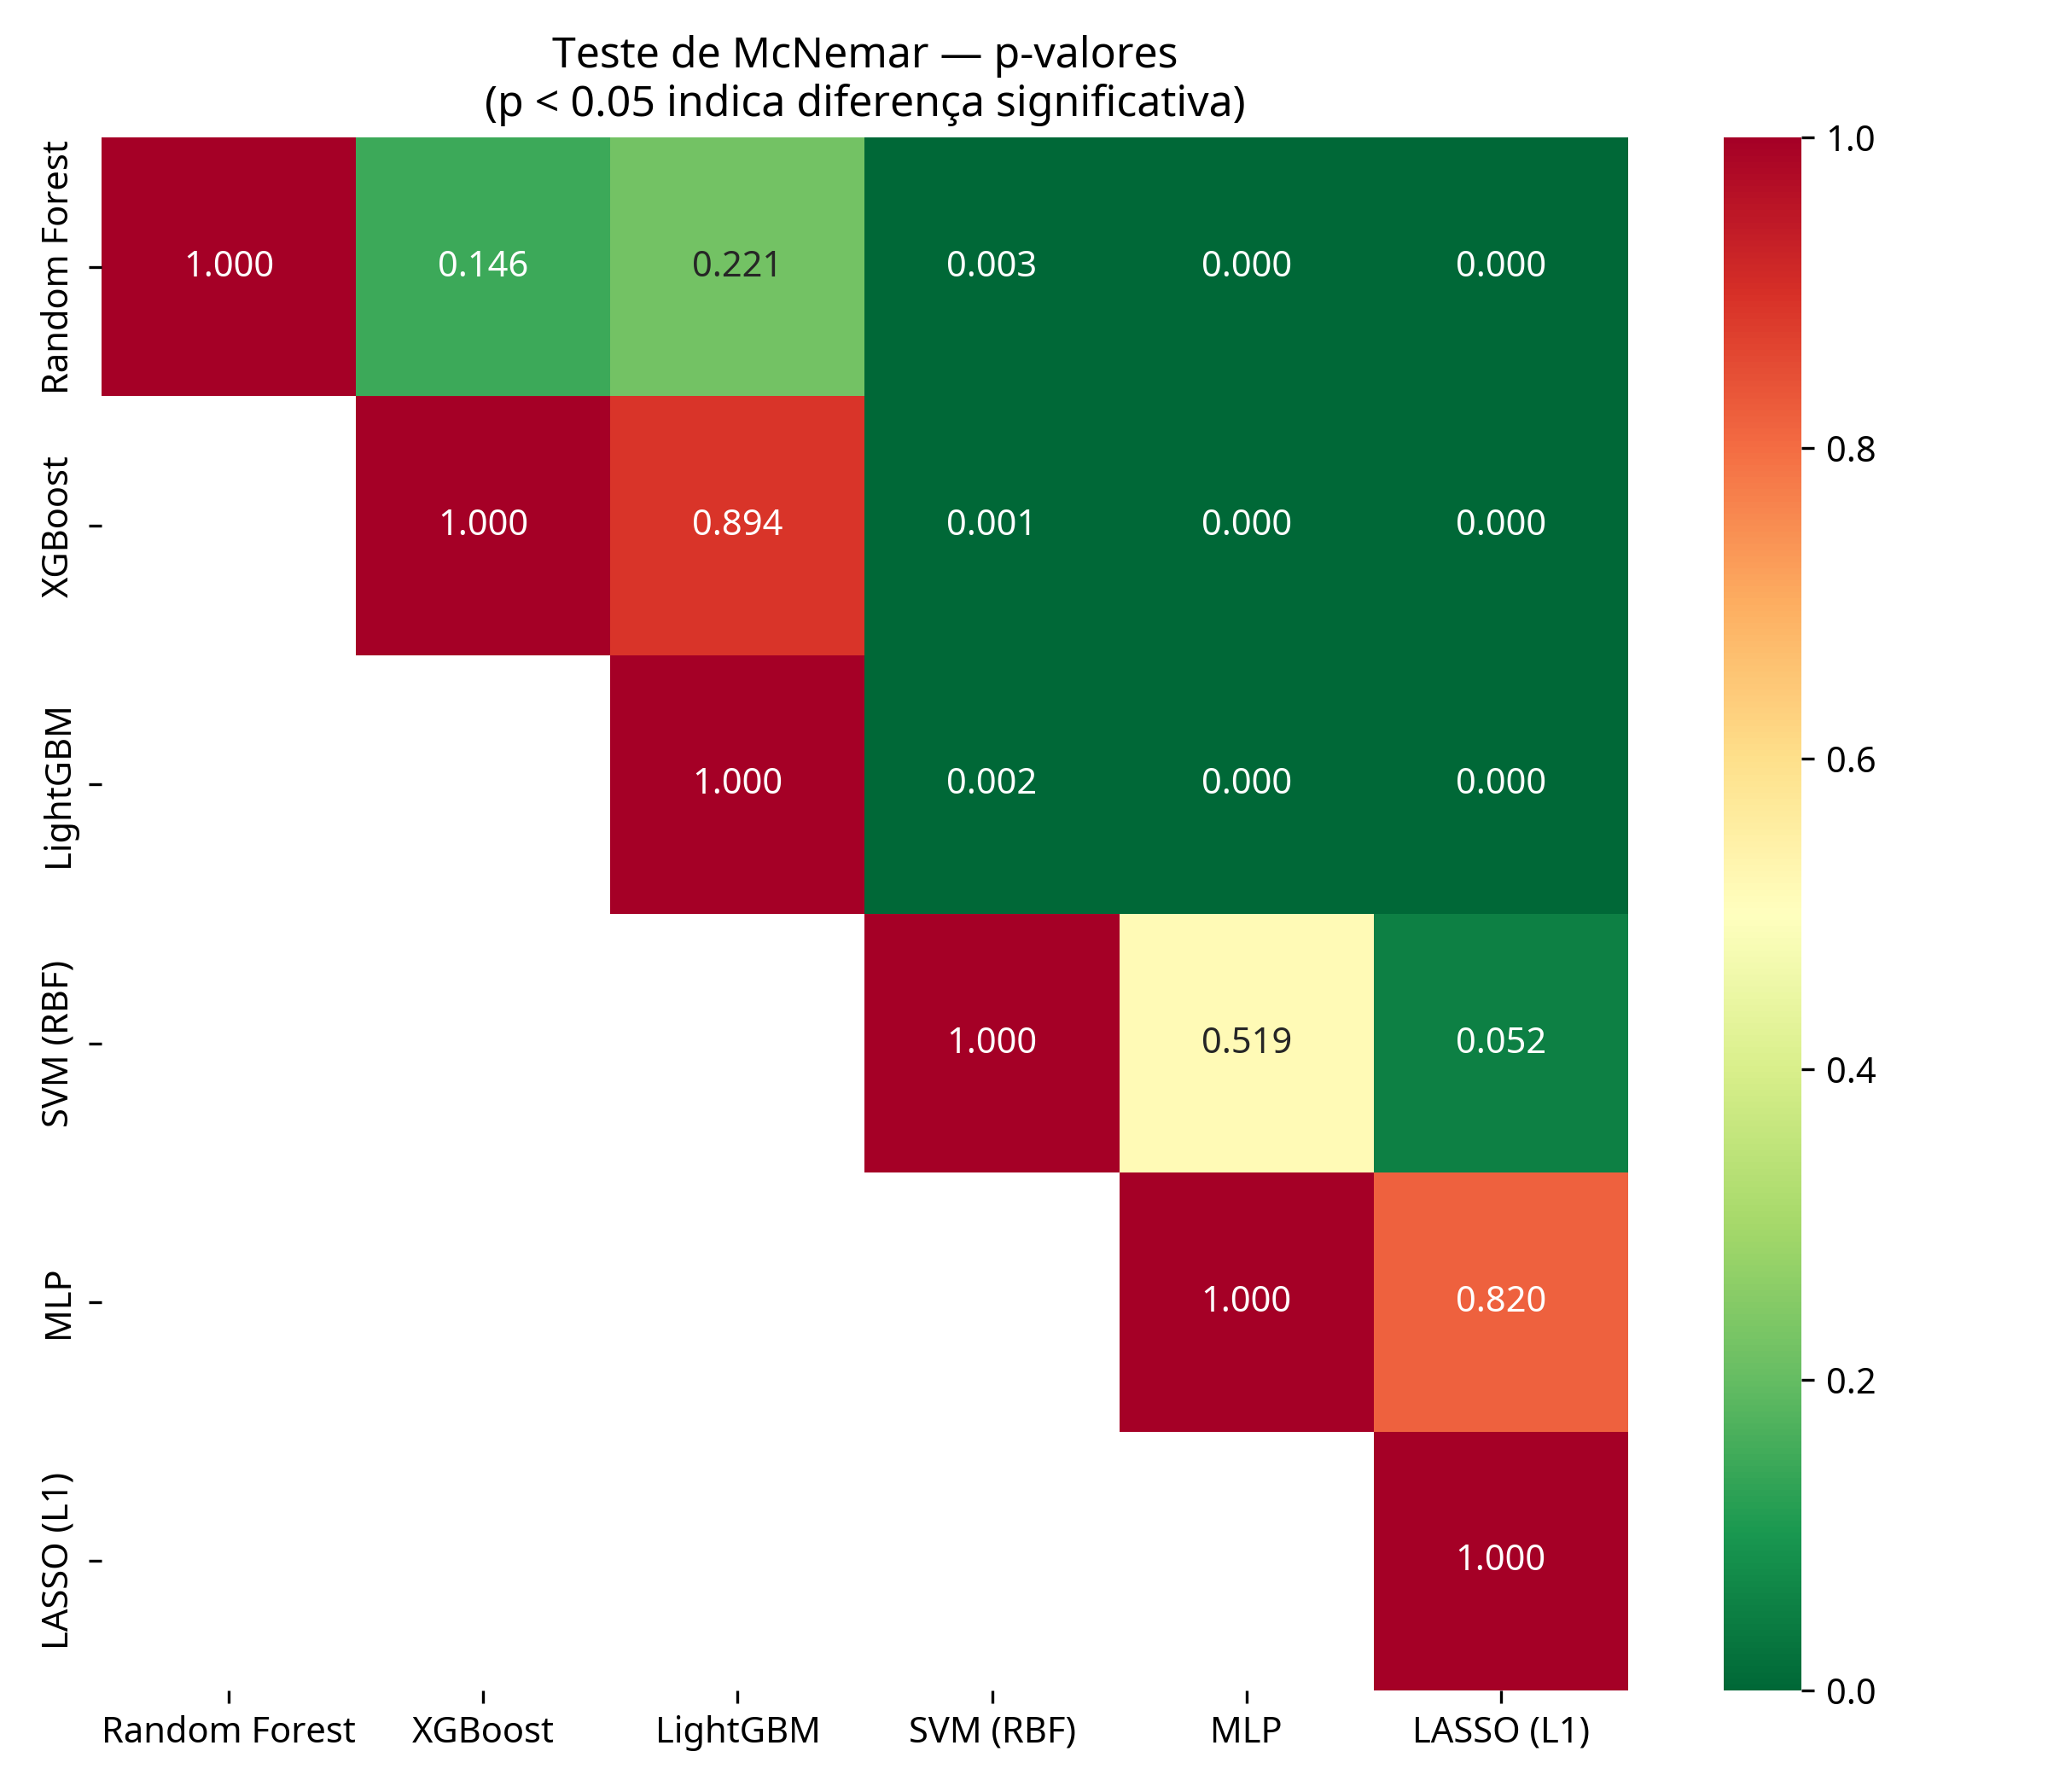
\includegraphics[width=\linewidth]{graficos/07_mcnemar_pvalues.png}
        \caption{Matriz de p-valores McNemar}
        \label{fig:mcnemar}
    \end{subfigure}
    \hfill
    \begin{subfigure}{0.48\textwidth}
        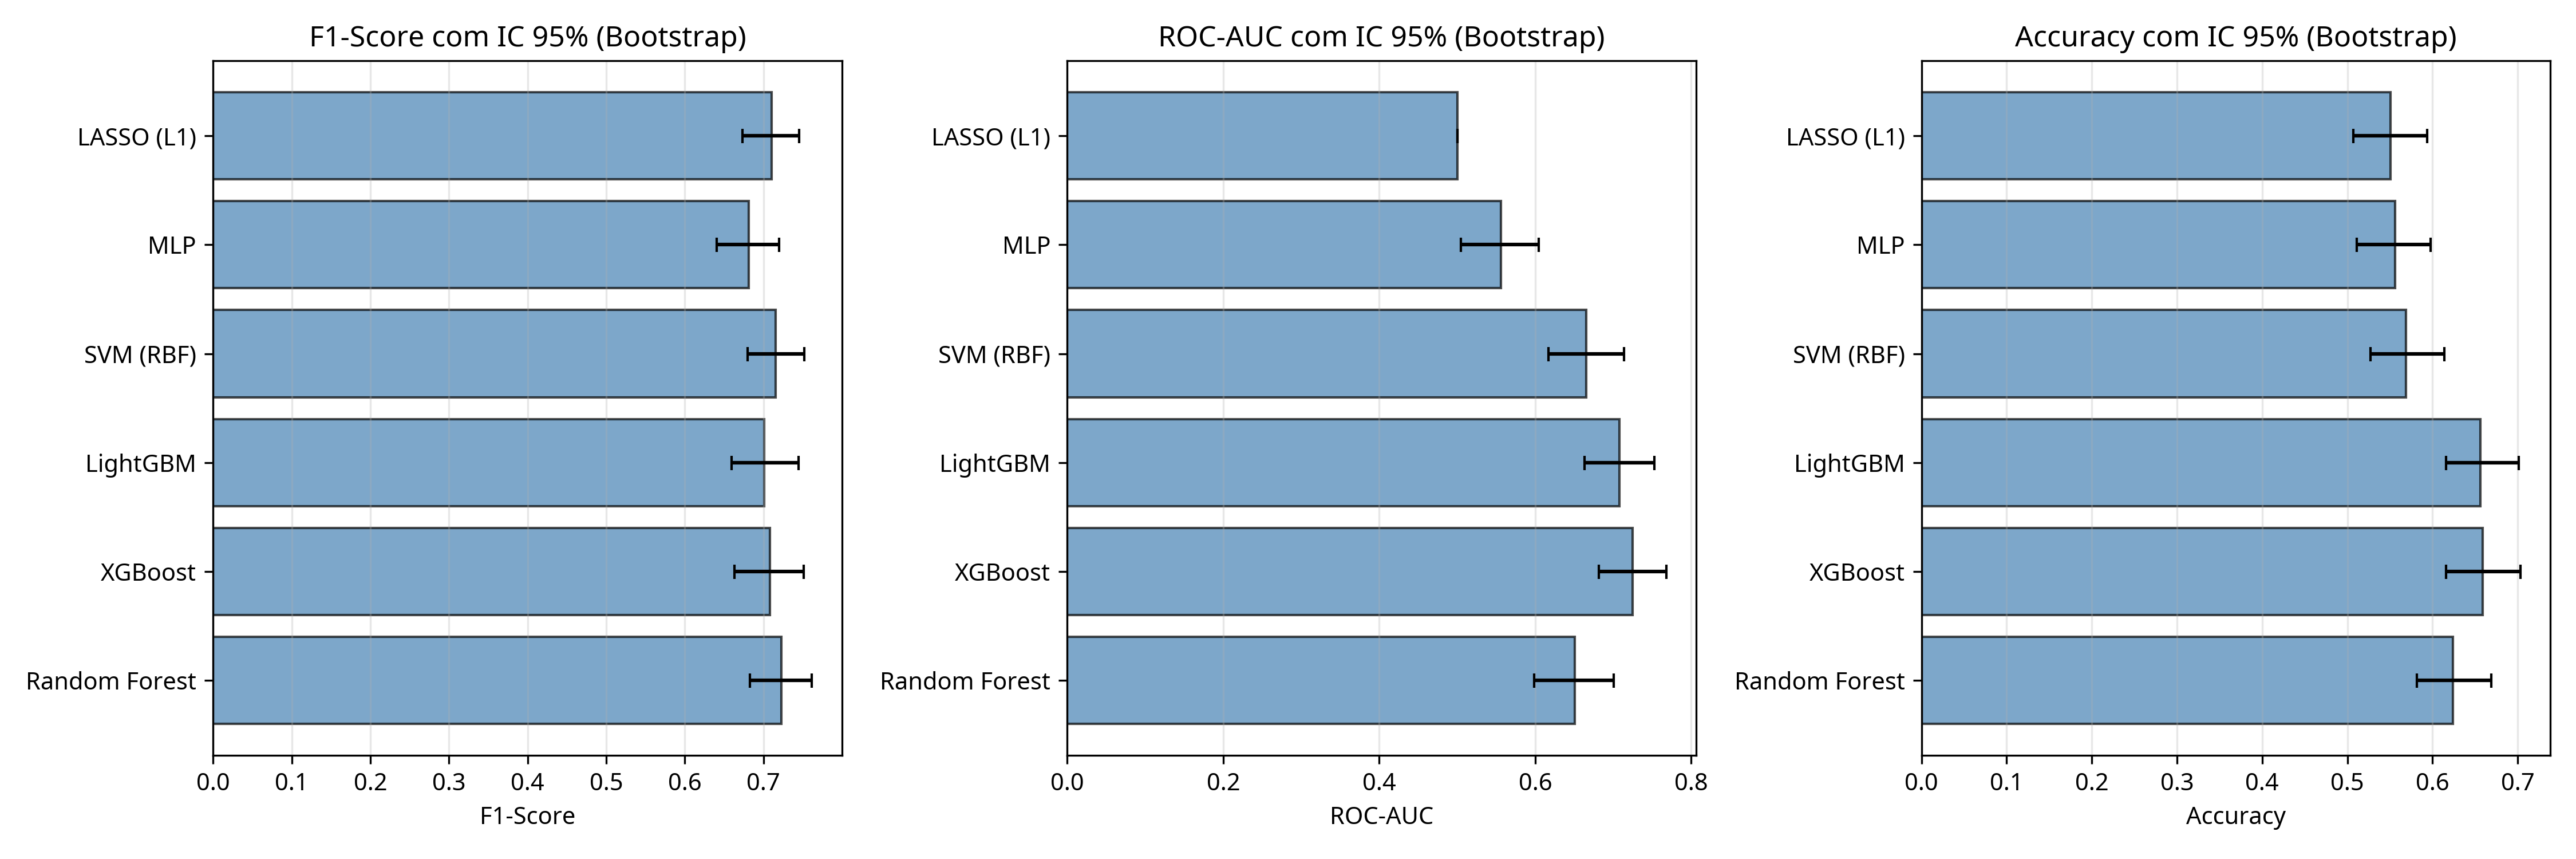
\includegraphics[width=\linewidth]{graficos/07_bootstrap_ci.png}
        \caption{IC 95\% \textit{bootstrap} das métricas}
        \label{fig:boot}
    \end{subfigure}
    \caption{Análise estatística comparativa. (a) Diferenças significativas entre modelos de árvore e MLP/LASSO; entre RF, XGBoost e LightGBM não há diferença significativa. (b) Sobreposição extensa dos intervalos confirma equivalência prática.}
\end{figure}

A conclusão metodológica é que, com o tamanho de amostra disponível e o controle de \textit{data leakage} adotado, \textbf{Random Forest, XGBoost e LightGBM são estatisticamente equivalentes} em termos de F1, com diferenças pontuais que devem ser interpretadas com cautela. A escolha do ``melhor modelo'' depende, portanto, do critério prático (recall vs. discriminação) e não de superioridade estatística inequívoca.

\section{Análise SHAP: Interpretabilidade Global e Local}
\label{sec:shap}

Para aprofundar a análise de interpretabilidade além da importância de \textit{features} agregada, foi aplicada a metodologia SHAP (\textit{SHapley Additive exPlanations}), que atribui a cada \textit{feature} de cada amostra uma contribuição aditiva à predição, com fundamentação na teoria de jogos cooperativos. A Figura \ref{fig:shap_summary} apresenta o \textit{summary plot} global das 20 \textit{features} mais relevantes para o Random Forest.

\begin{figure}[H]
    \centering
    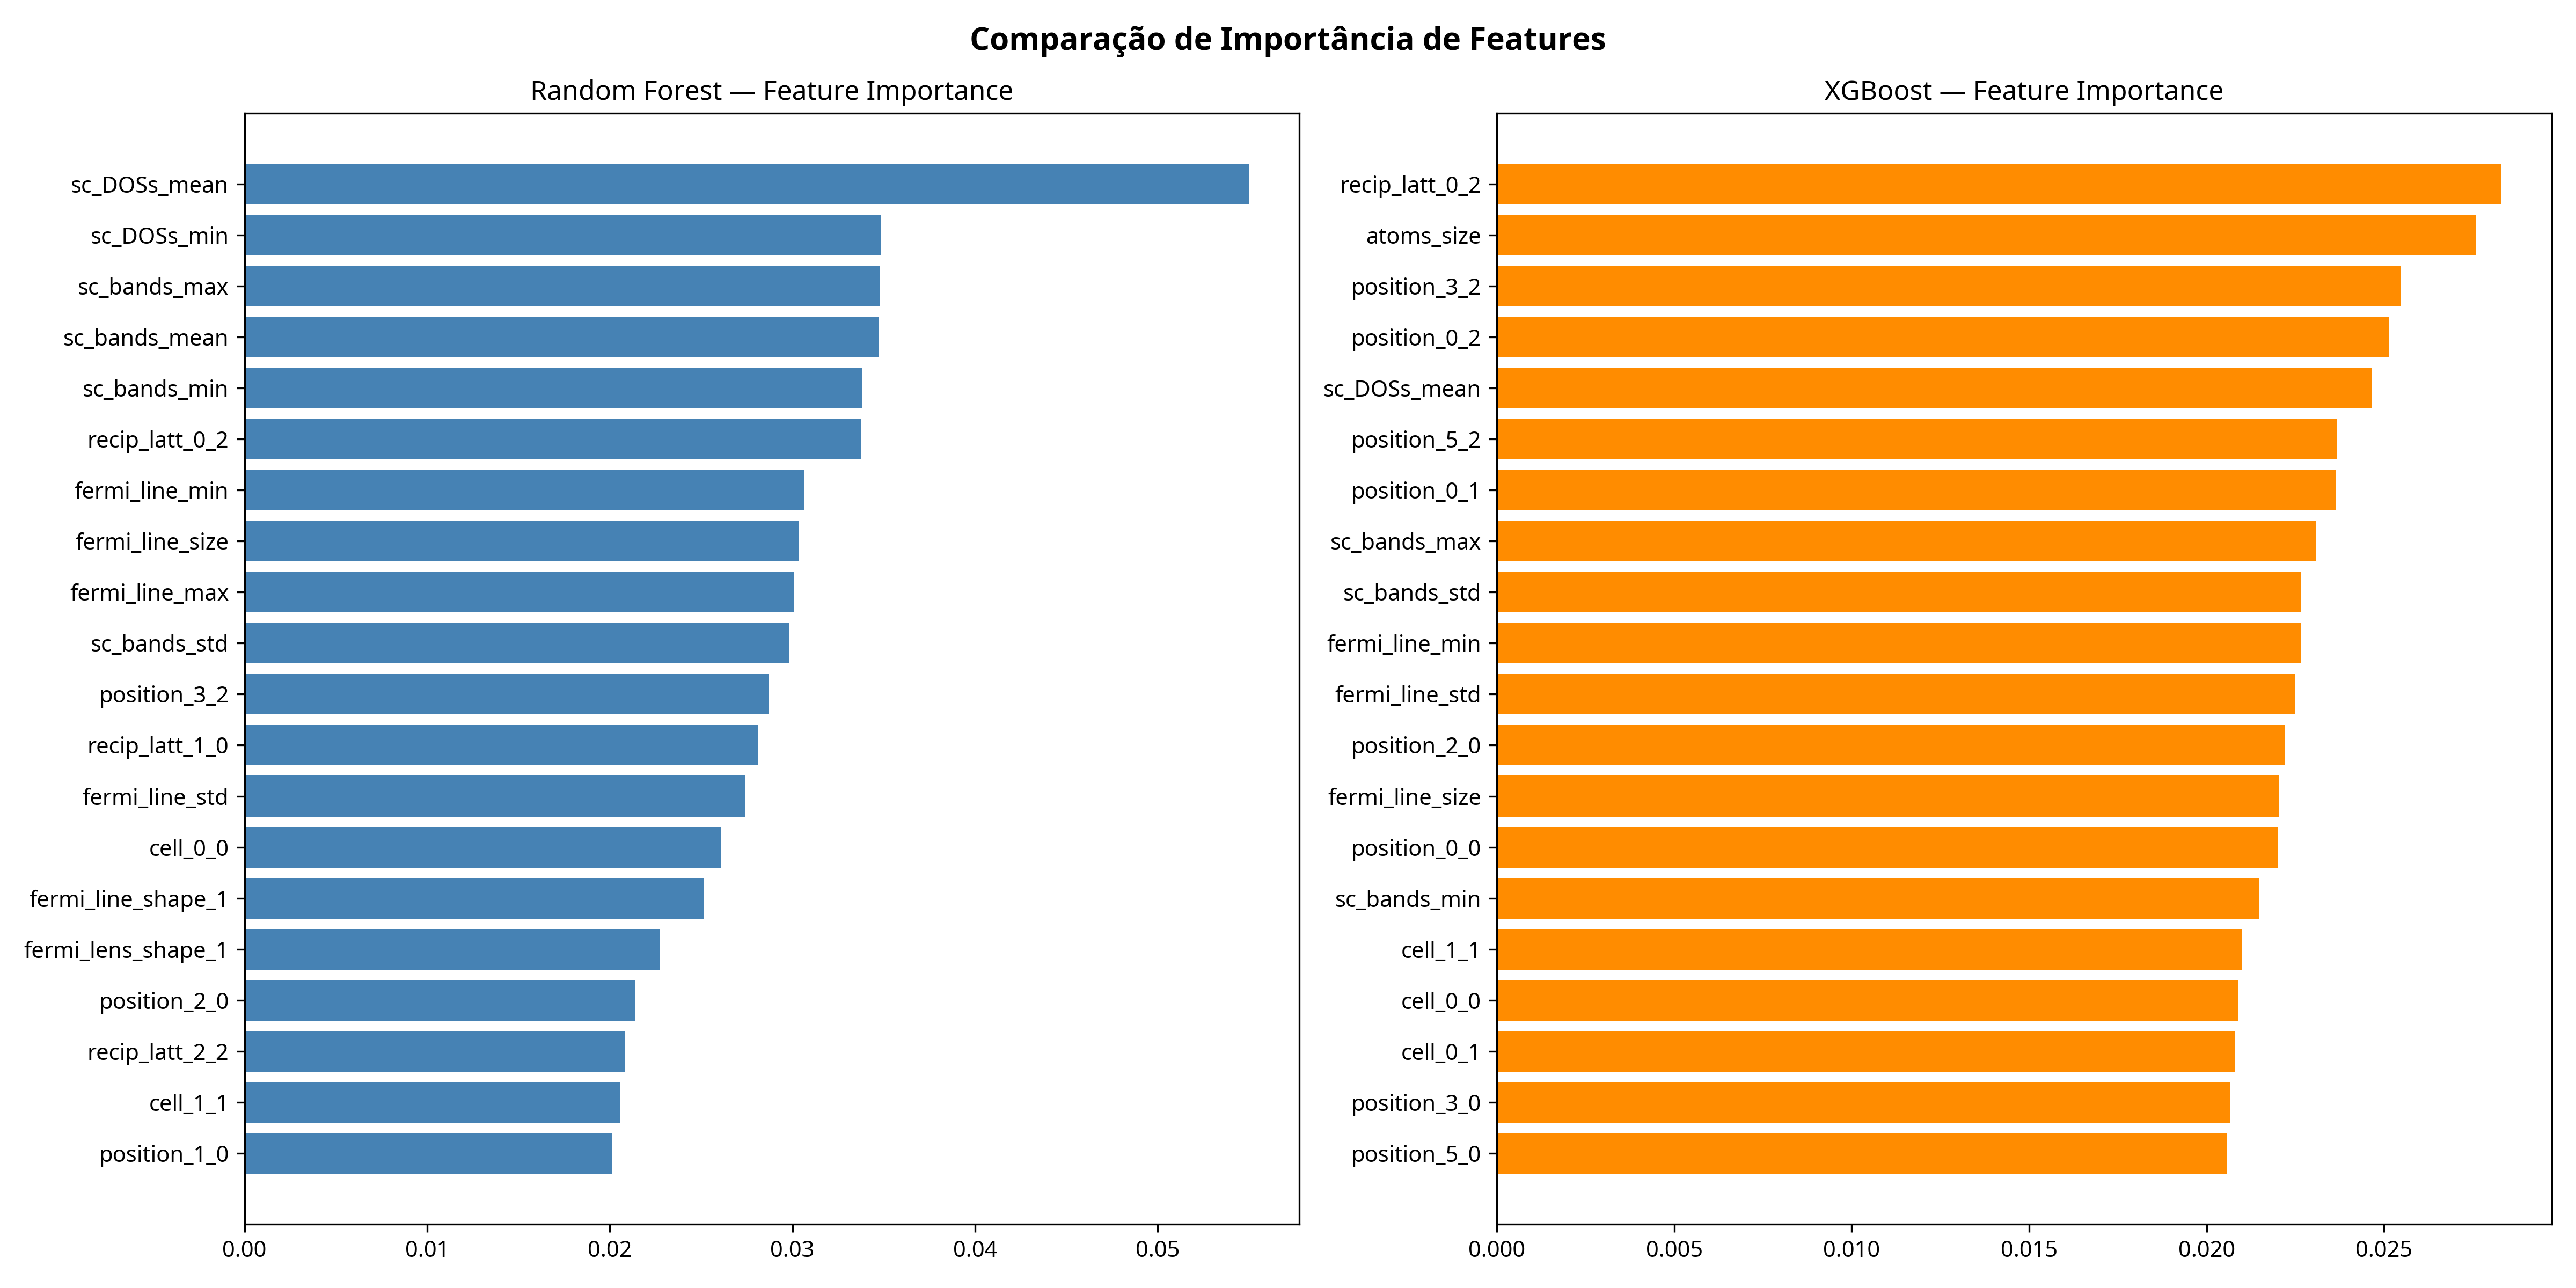
\includegraphics[width=0.95\textwidth]{graficos/24_shap_summary.png}
    \caption{Diagrama SHAP \textit{summary} (\textit{beeswarm}) das 20 \textit{features} mais importantes para o Random Forest. A posição horizontal indica a contribuição da \textit{feature} para a predição (positivo $\to$ supercondutor); a cor indica o valor da \textit{feature} (vermelho = alto, azul = baixo).}
    \label{fig:shap_summary}
\end{figure}

A análise SHAP confirma e refina os achados da importância clássica: as \textit{features} \texttt{sc\_DOSs\_mean} e \texttt{sc\_DOSs\_min}, bem como descritores da estrutura de bandas no nível de Fermi (\texttt{sc\_bands\_*}), dominam as predições. Valores altos da DOS média estão sistematicamente associados a contribuições SHAP positivas (deslocando a predição para a classe ``supercondutor''), em consonância direta com a expectativa BCS.

\section{Calibração de Probabilidades}
\label{sec:calibracao}

Além da capacidade discriminativa medida pelo ROC-AUC, é importante avaliar se as probabilidades preditas pelos modelos refletem adequadamente as frequências observadas --- uma propriedade conhecida como \textit{calibração}. Um modelo bem calibrado é fundamental quando suas predições são utilizadas como entrada de processos de decisão (e.g., priorização de candidatos para síntese experimental).

A Figura \ref{fig:calib} apresenta o \textit{reliability diagram} dos dois melhores modelos (Random Forest e XGBoost), junto com seus \textit{Brier scores}.

\begin{figure}[H]
    \centering
    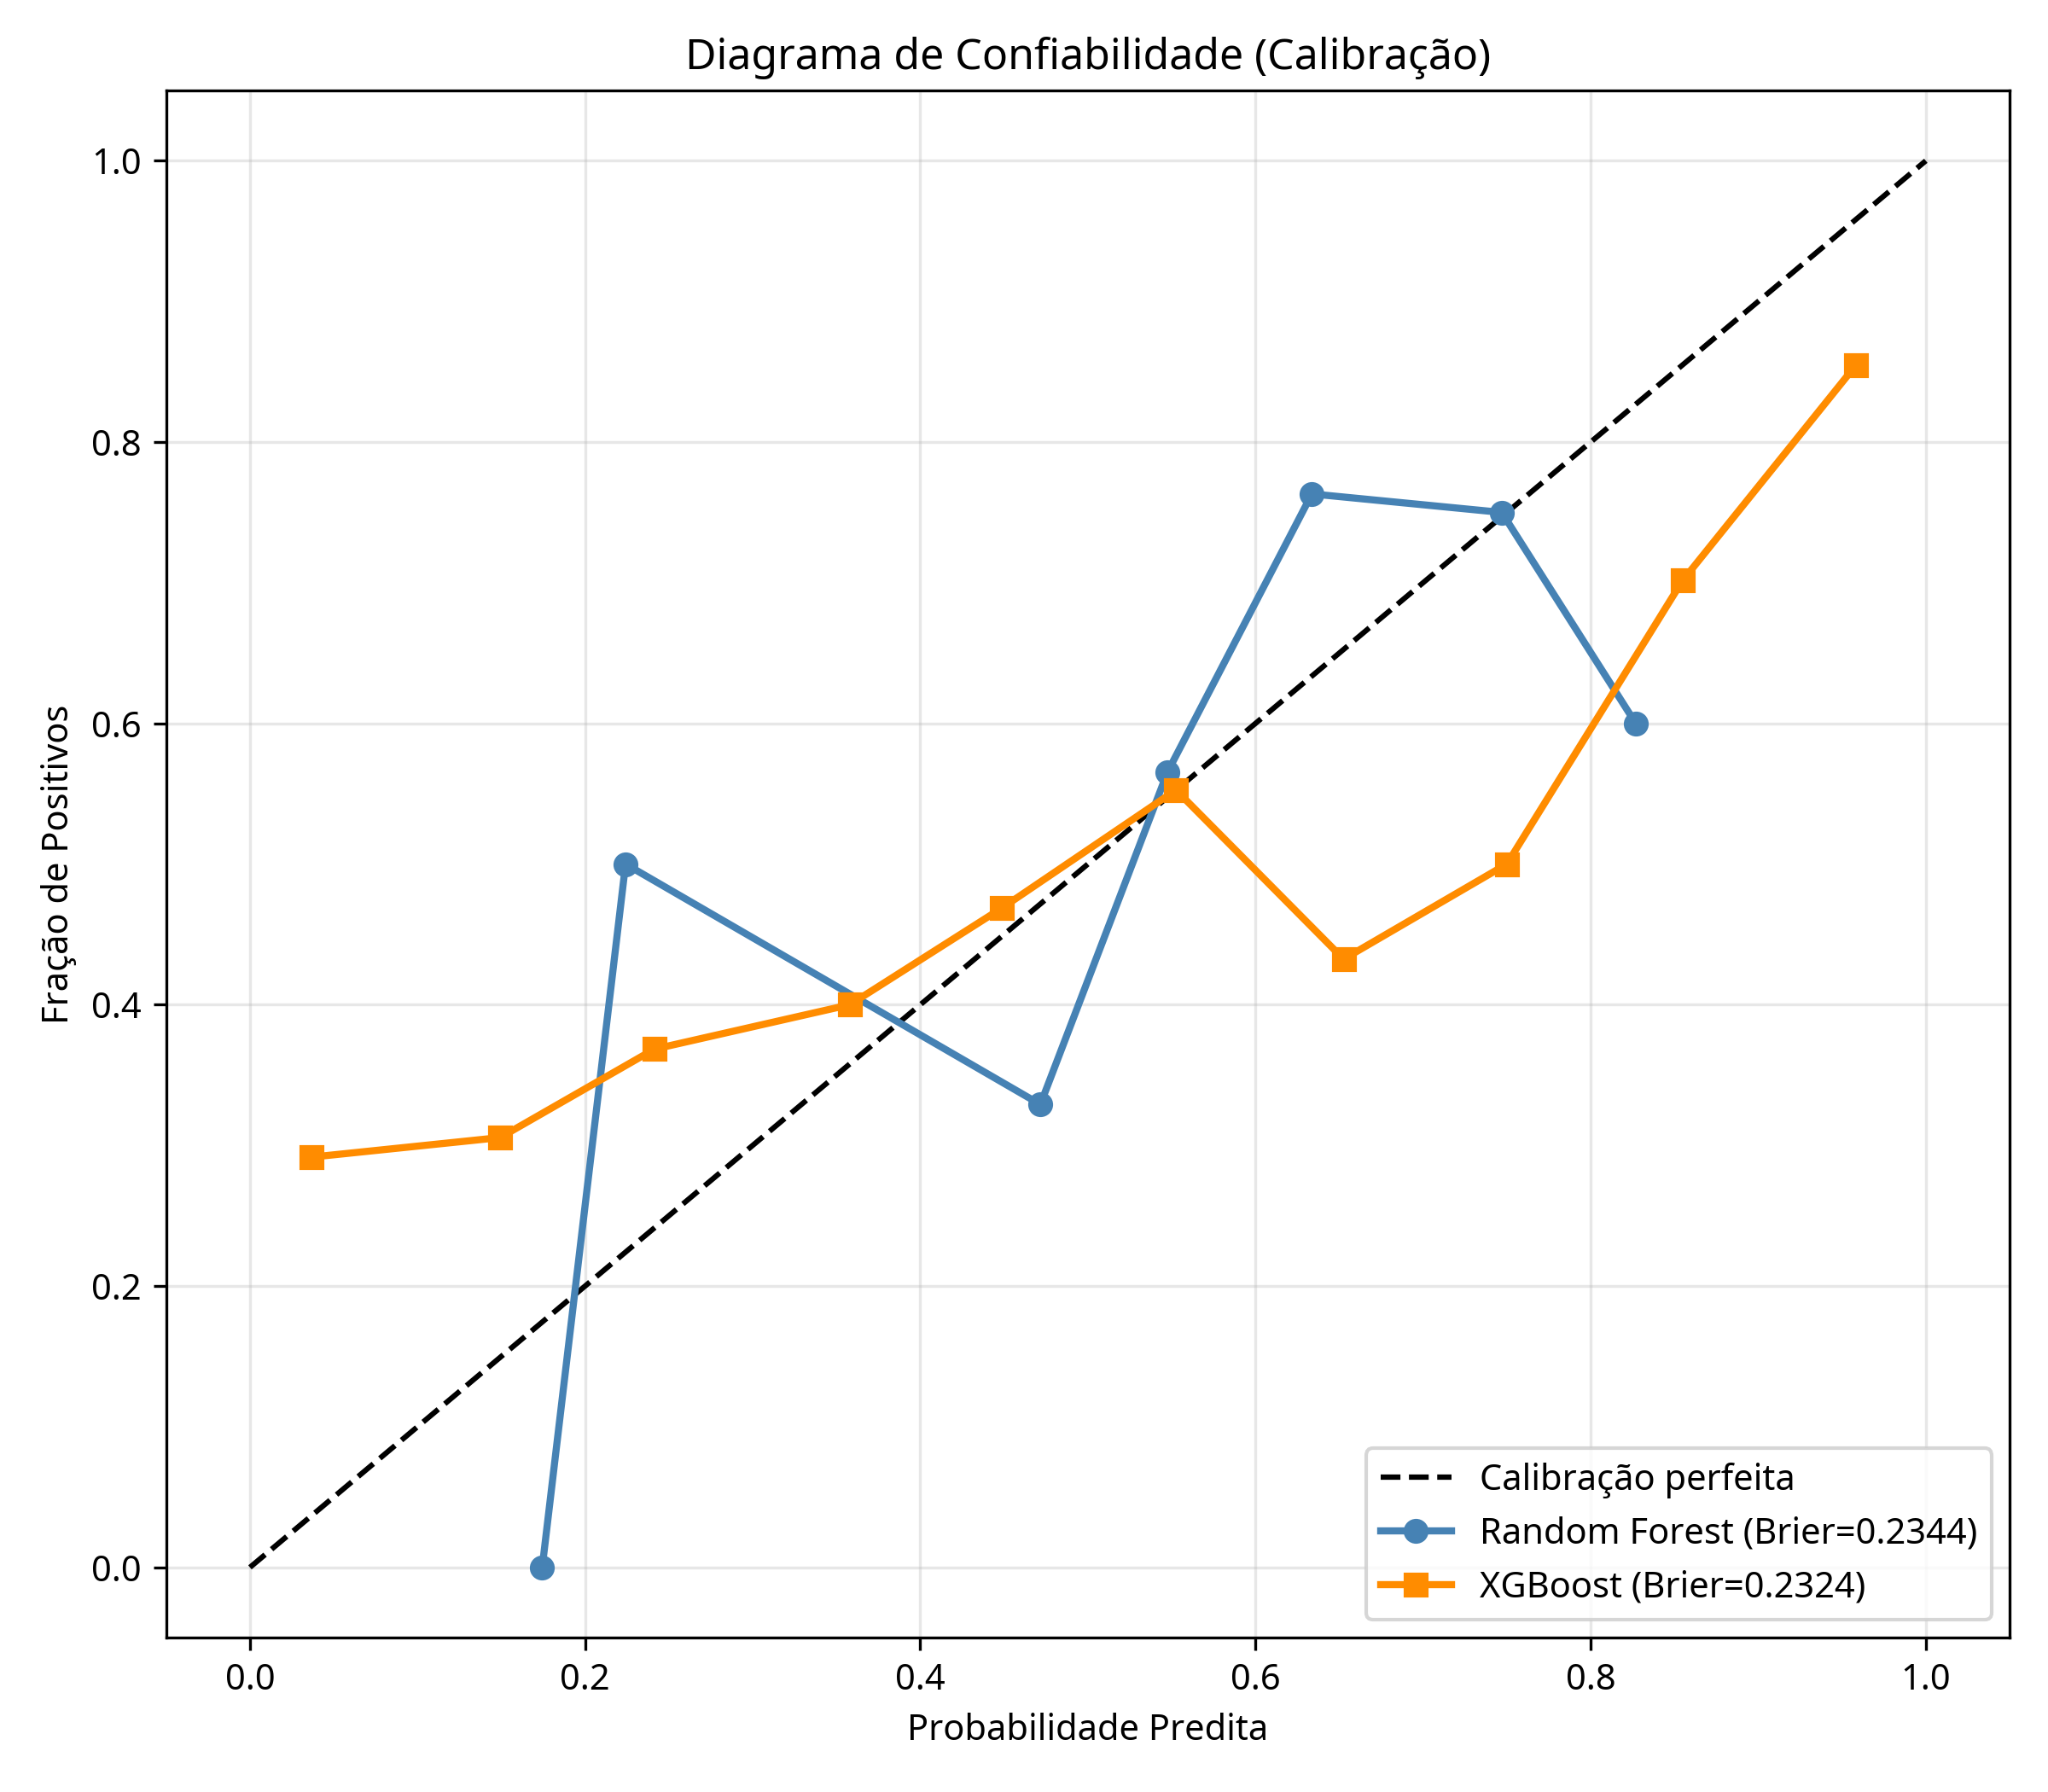
\includegraphics[width=0.7\textwidth]{graficos/27_calibration.png}
    \caption{Diagrama de calibração (\textit{reliability diagram}) para Random Forest e XGBoost. A linha diagonal indica calibração perfeita. \textit{Brier score}: RF = 0.234, XGBoost = 0.232 (menor é melhor).}
    \label{fig:calib}
\end{figure}

Ambos os modelos apresentam \textit{Brier scores} similares (RF: 0.234, XGBoost: 0.232), com calibração razoável mas distante da ideal. As curvas exibem leve sobre-confiança em probabilidades intermediárias. Para uso prático em triagem, recomenda-se a aplicação de técnicas de calibração \textit{a posteriori}, como Platt scaling ou regressão isotônica.

\section{Curva de Aprendizado}
\label{sec:learning}

A curva de aprendizado (Figura \ref{fig:learning}) mostra o F1-Score do Random Forest e do XGBoost em função do tamanho do conjunto de treino (10\%, 25\%, 50\%, 75\% e 100\%). Esta análise informa se mais dados conduziriam a melhor desempenho ou se o regime de saturação já foi atingido.

\begin{figure}[H]
    \centering
    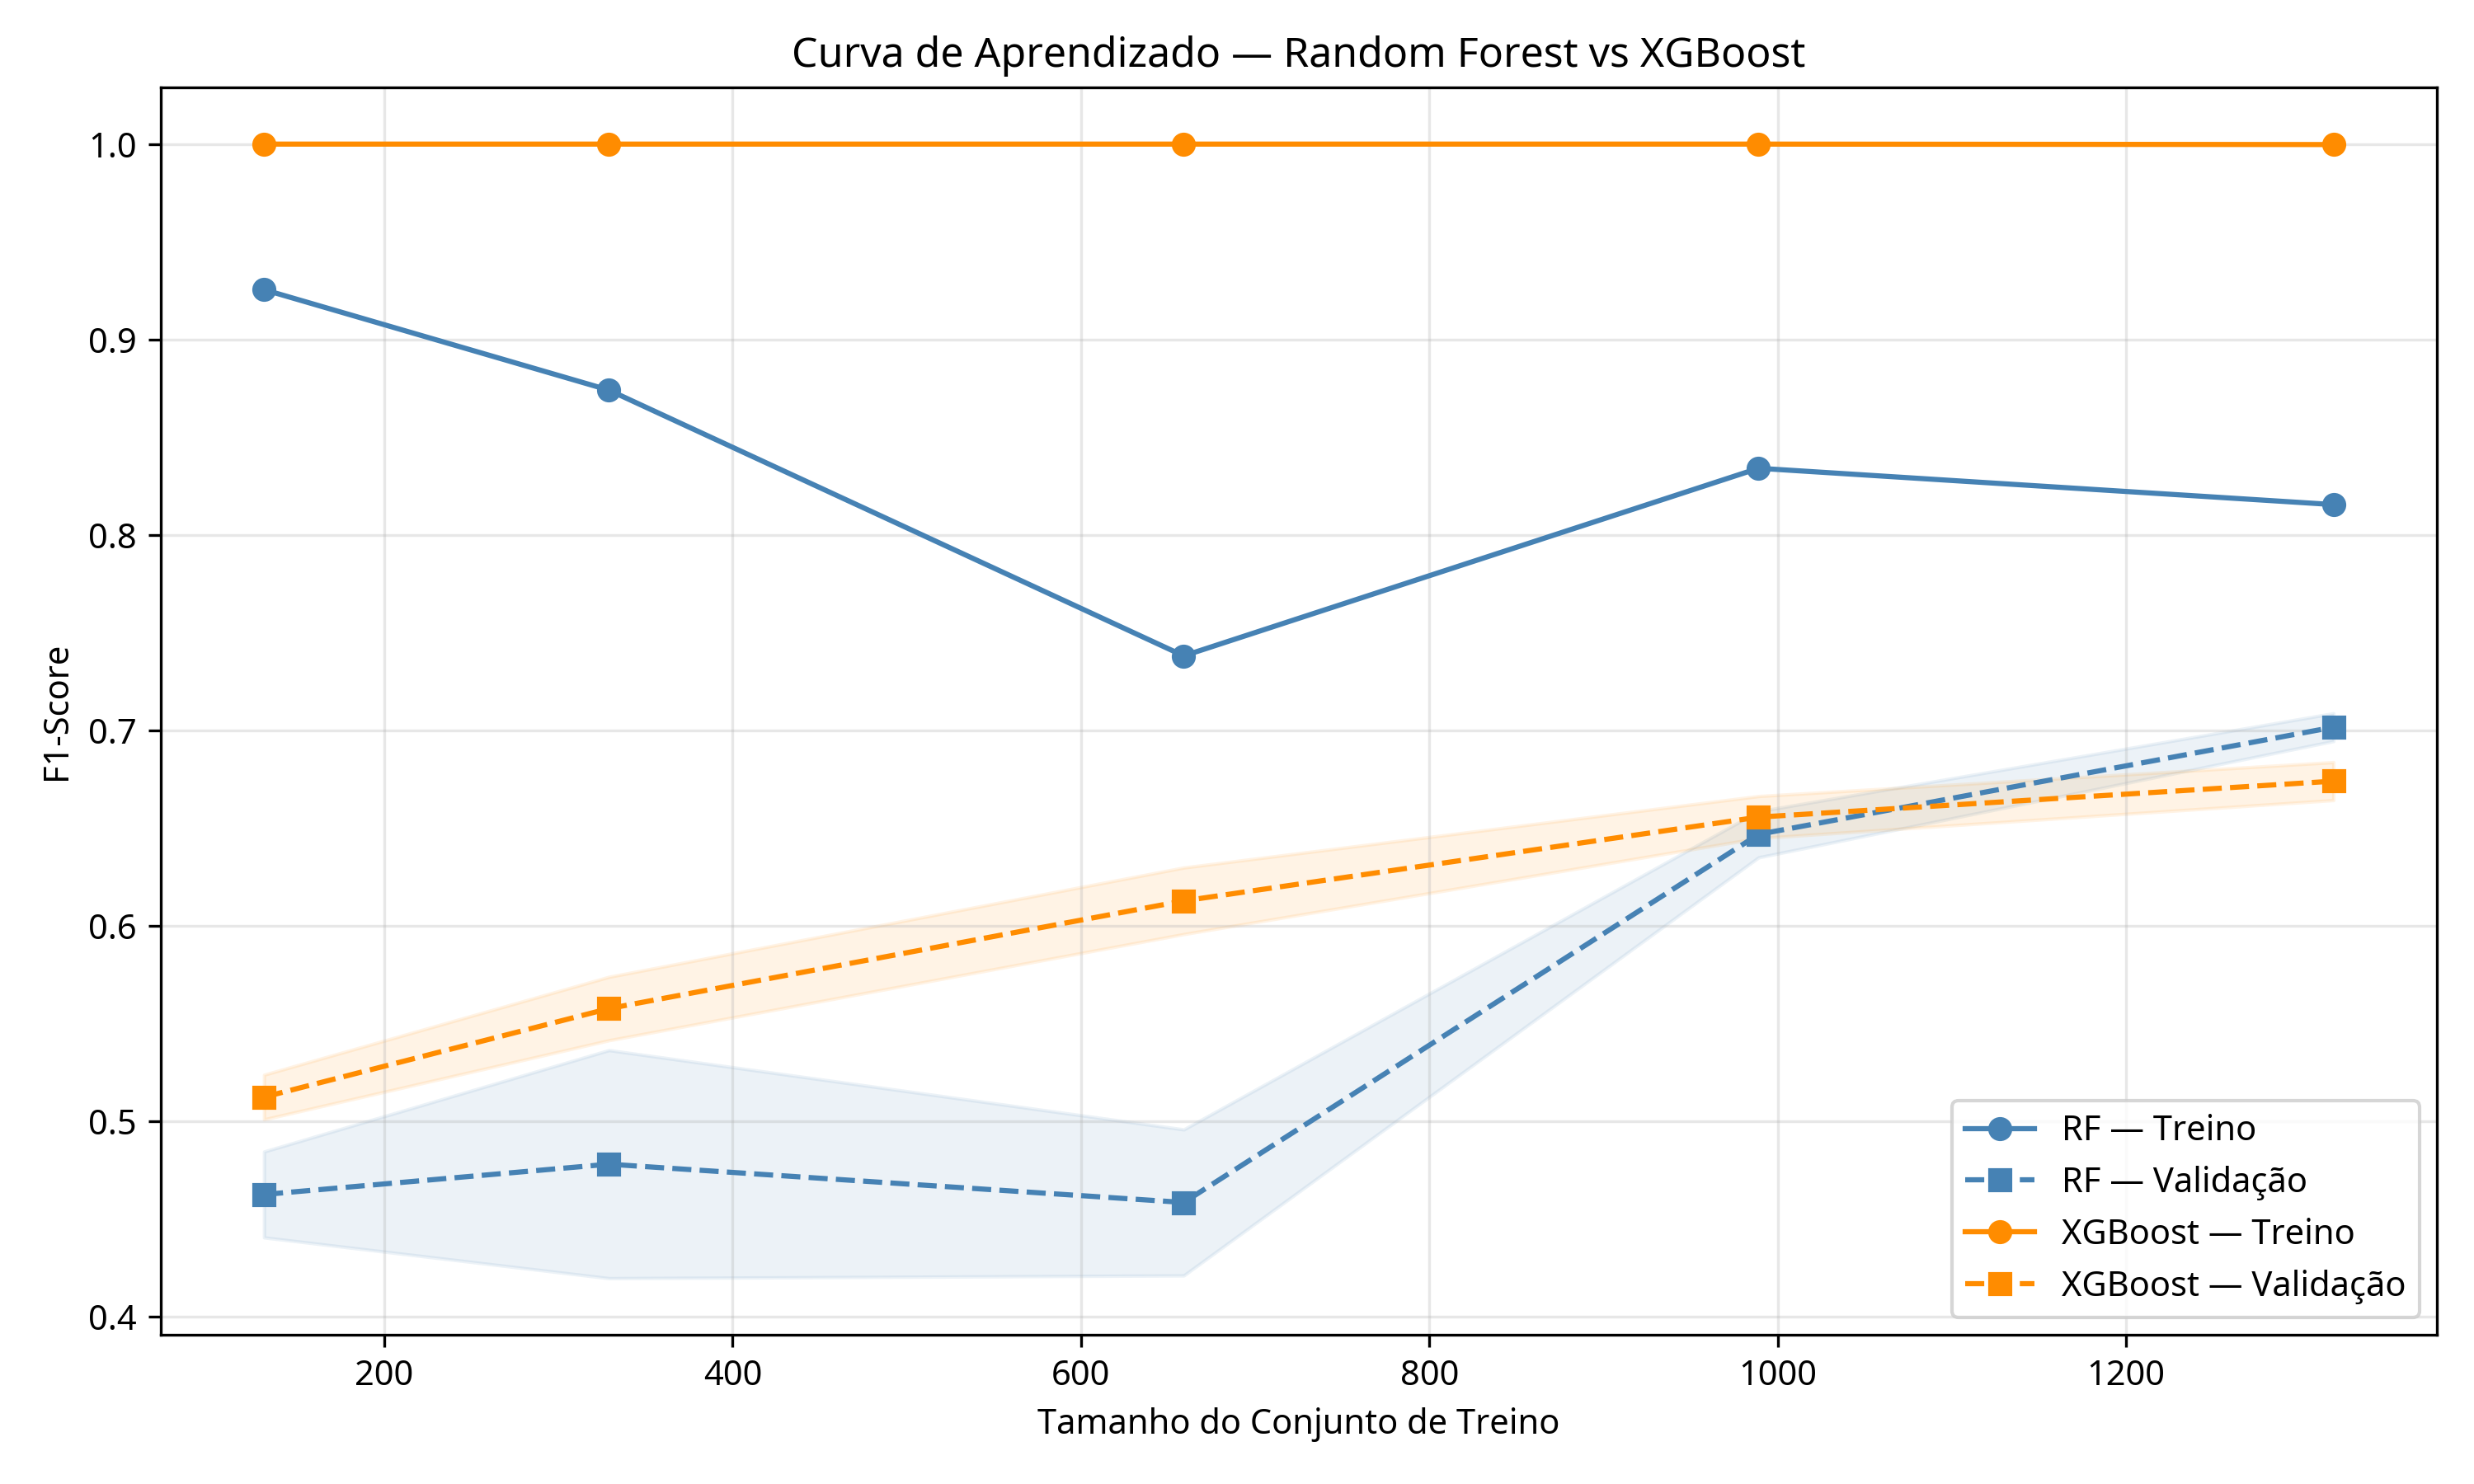
\includegraphics[width=0.7\textwidth]{graficos/28_learning_curve.png}
    \caption{Curva de aprendizado: F1-Score em função do tamanho do treino. A diferença pequena entre as curvas de treino e validação no extremo direito indica baixo \textit{overfitting}; a inclinação remanescente sugere que dados adicionais ainda trariam ganhos modestos.}
    \label{fig:learning}
\end{figure}

O comportamento observado --- ganho contínuo, ainda que decrescente, com o tamanho do treino --- sugere que o desempenho atual não está saturado e que a expansão do banco de dados (e.g., agregando o NIMS SuperCon e outros repositórios) poderia trazer melhorias incrementais nos modelos. Esta observação reforça a discussão das Limitações (Seção \ref{sec:limitacoes}).

\section{Análise de Interpretabilidade: Partial Dependence Plots}

Para entender \textit{como} a probabilidade de classificação varia com as \textit{features} mais importantes, geramos Partial Dependence Plots (PDPs). Os PDPs mostram o efeito marginal de uma \textit{feature} na predição do modelo, marginalizando sobre os valores das outras \textit{features}.

\begin{figure}[H]
    \centering
    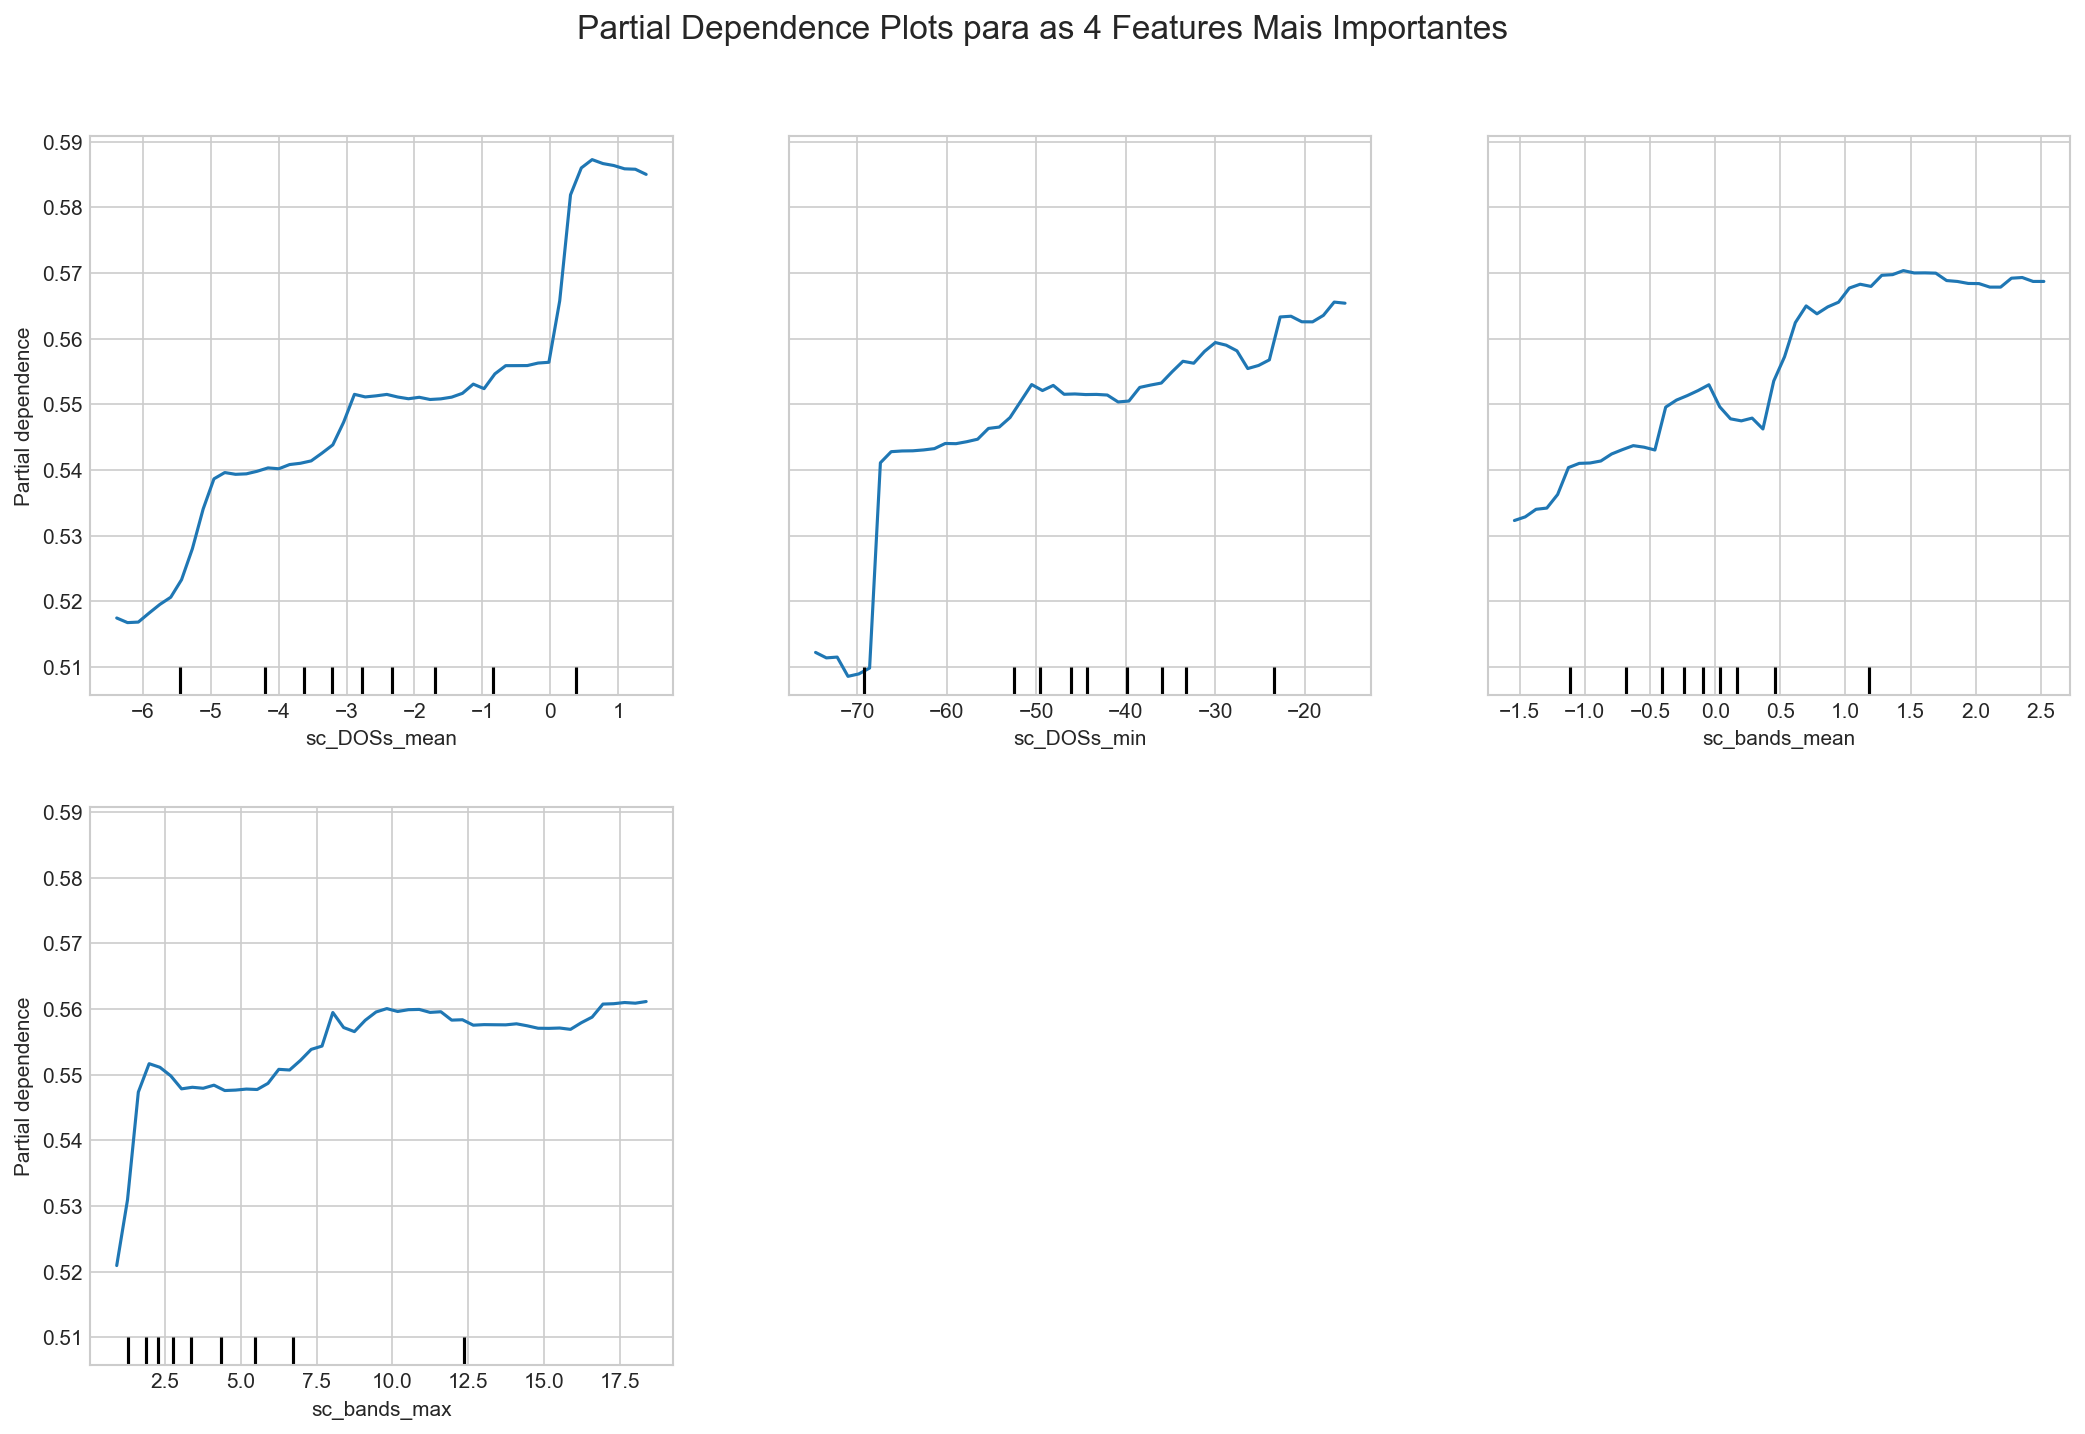
\includegraphics[width=\textwidth]{graficos/18_partial_dependence_plots.png}
    \caption{Partial Dependence Plots para as 4 \textit{features} mais importantes do modelo Random Forest.}
    \label{fig:pdp}
\end{figure}

A Figura \ref{fig:pdp} revela relações claras e fisicamente interpretáveis:
\begin{itemize}
    \item \textbf{\texttt{sc\_DOSs\_mean}:} A probabilidade de ser supercondutor aumenta monotonicamente com a densidade de estados média. Isso é diretamente consistente com a teoria BCS.
    \item \textbf{\texttt{sc\_DOSs\_min}:} A probabilidade aumenta com valores menos negativos (mais próximos de zero) do mínimo da DOS, sugerindo que materiais com uma DOS mais uniforme e alta são favorecidos.
    \item \textbf{\texttt{sc\_bands\_mean} e \texttt{sc\_bands\_std}:} A probabilidade aumenta com valores mais altos dessas \textit{features}, indicando que a estrutura de bandas (energia e dispersão) no nível de Fermi é um fator importante.
\end{itemize}

\section{Análise de Erro}
\label{sec:erro}

Para entender as limitações do modelo, realizamos uma análise detalhada dos erros de classificação. A Figura \ref{fig:analise_erro} mostra a distribuição da temperatura crítica para os Falsos Negativos (supercondutores que o modelo classificou incorretamente como não-supercondutores).

\begin{figure}[H]
    \centering
    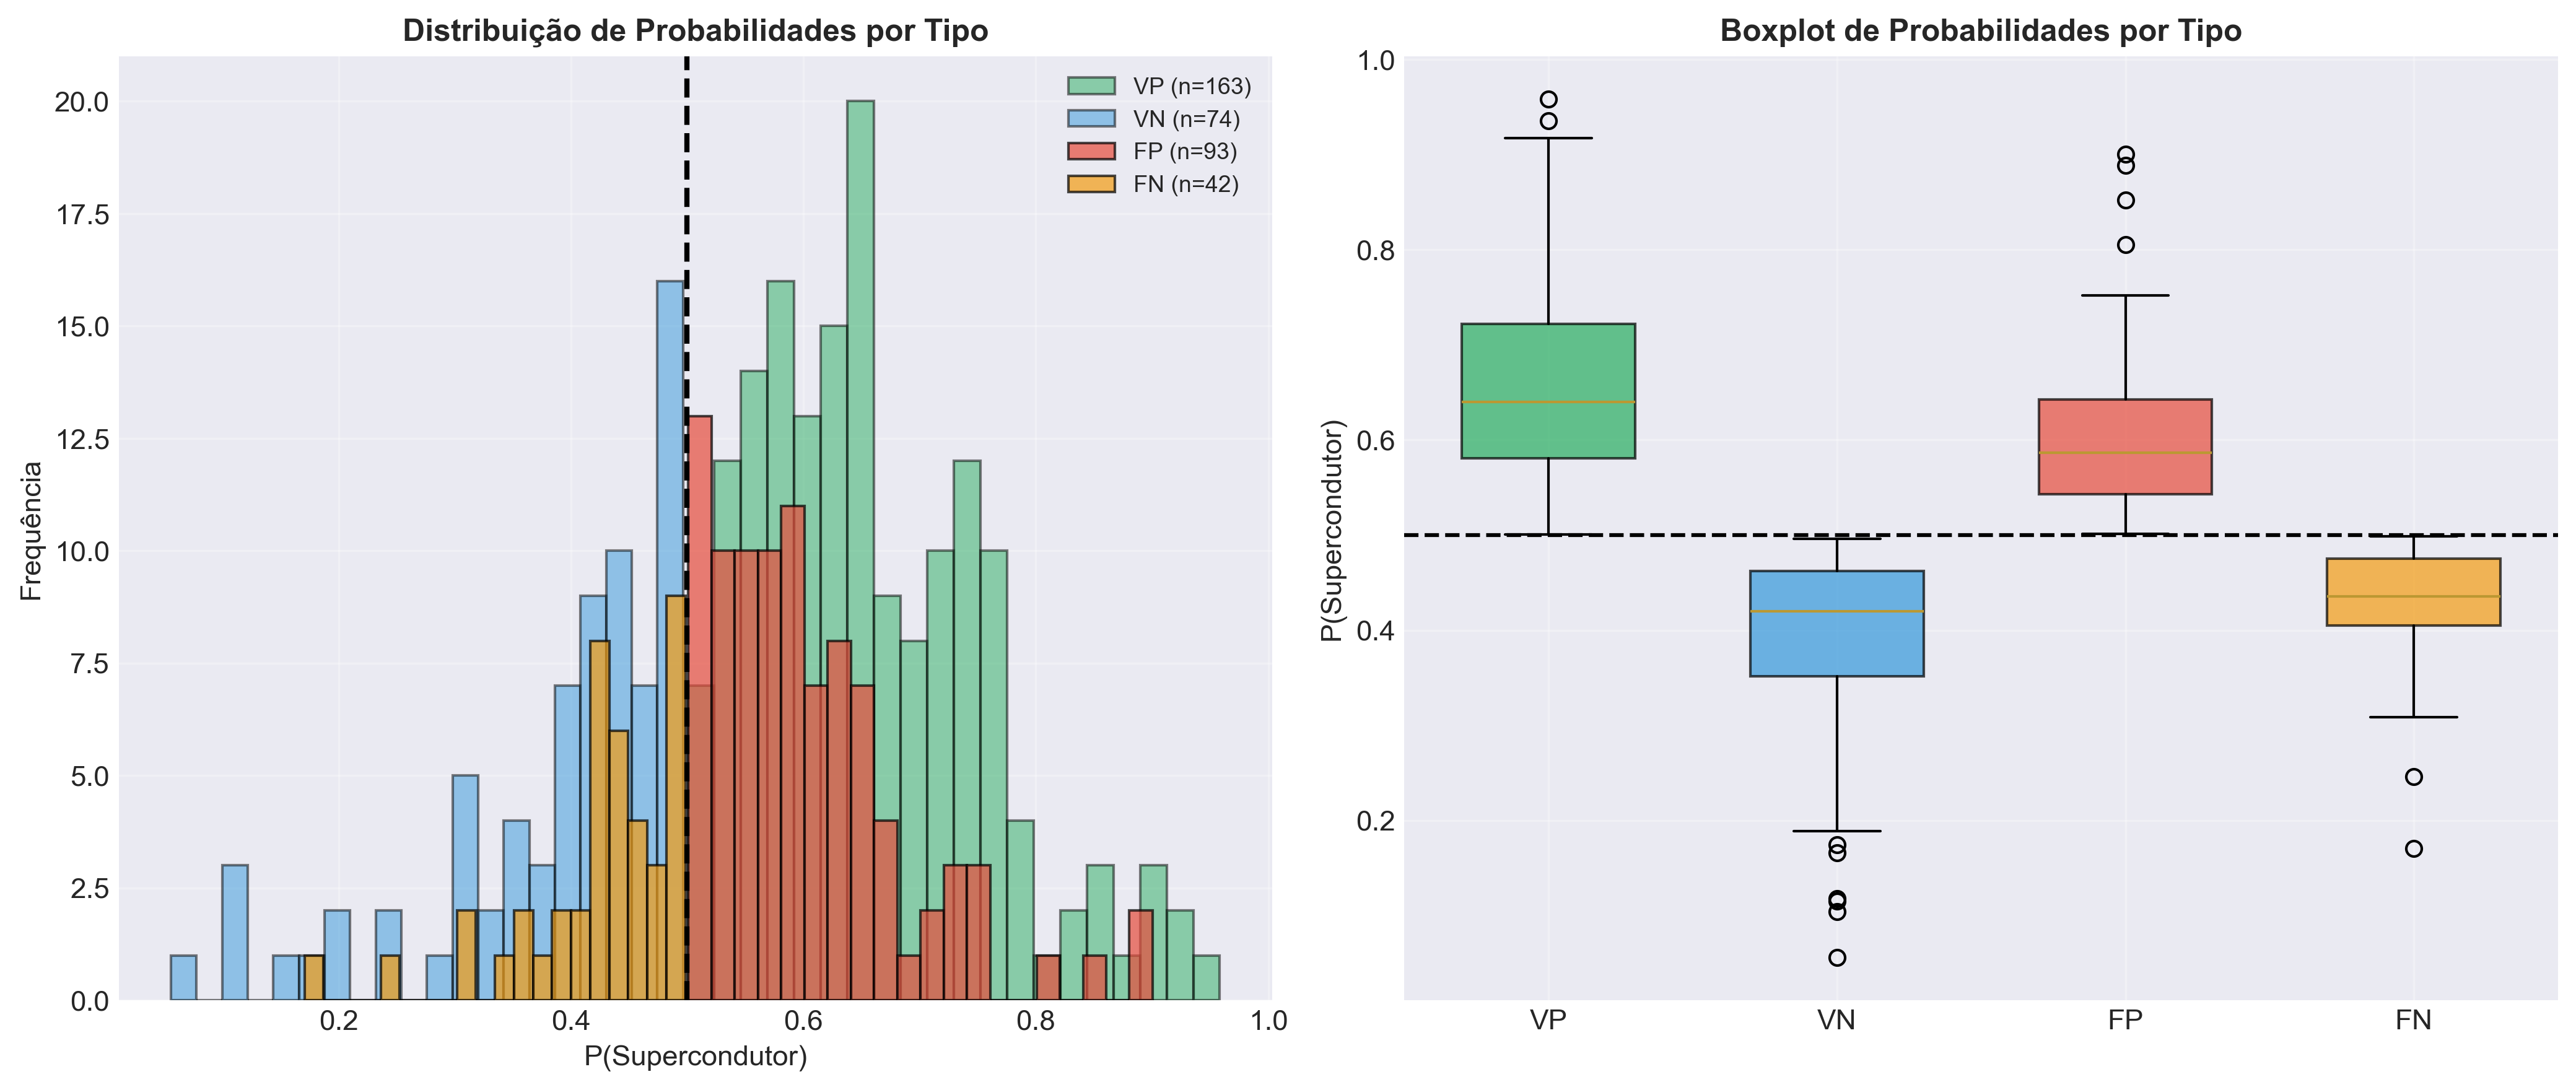
\includegraphics[width=\textwidth]{graficos/08_analise_erro.png}
    \caption{Análise de erro do modelo Random Forest. À esquerda, a distribuição de $T_c$ para os Falsos Negativos. À direita, a distribuição da \textit{feature} \texttt{sc\_DOSs\_mean} para predições corretas e incorretas.}
    \label{fig:analise_erro}
\end{figure}

A análise revela um padrão importante: a mediana de $T_c$ para os Falsos Negativos é de apenas \textbf{2.35 K} (com 54 falsos negativos em 495 amostras de teste). Isso indica que o modelo tem maior dificuldade em identificar \textbf{supercondutores convencionais de baixa temperatura}. Uma possível explicação física é que esses materiais, com $T_c$ muito baixo, possuem um gap supercondutor pequeno e propriedades eletrônicas (como a DOS) que são muito similares às de materiais não-supercondutores. Os descritores disponíveis podem não ser suficientes para distinguir esses casos limítrofes.

O gráfico à direita da Figura \ref{fig:analise_erro} mostra que as predições incorretas (em vermelho) têm uma distribuição de \texttt{sc\_DOSs\_mean} que se sobrepõe significativamente com as predições corretas (em verde), mas com uma concentração ligeiramente maior em valores intermediários. Isso sugere que a região de "fronteira" no espaço de \textit{features} é onde o modelo tem mais incerteza.

\section{Validação Cruzada}

Para garantir a robustez dos resultados, foi realizada uma validação cruzada de 5 folds. Os resultados, mostrados na Figura \ref{fig:cv}, são consistentes com a avaliação no conjunto de teste. O Random Forest mantém o melhor desempenho médio (F1-Score de 0.706), com um desvio padrão baixo, indicando que seu desempenho é estável em diferentes subconjuntos dos dados.

\begin{figure}[H]
    \centering
    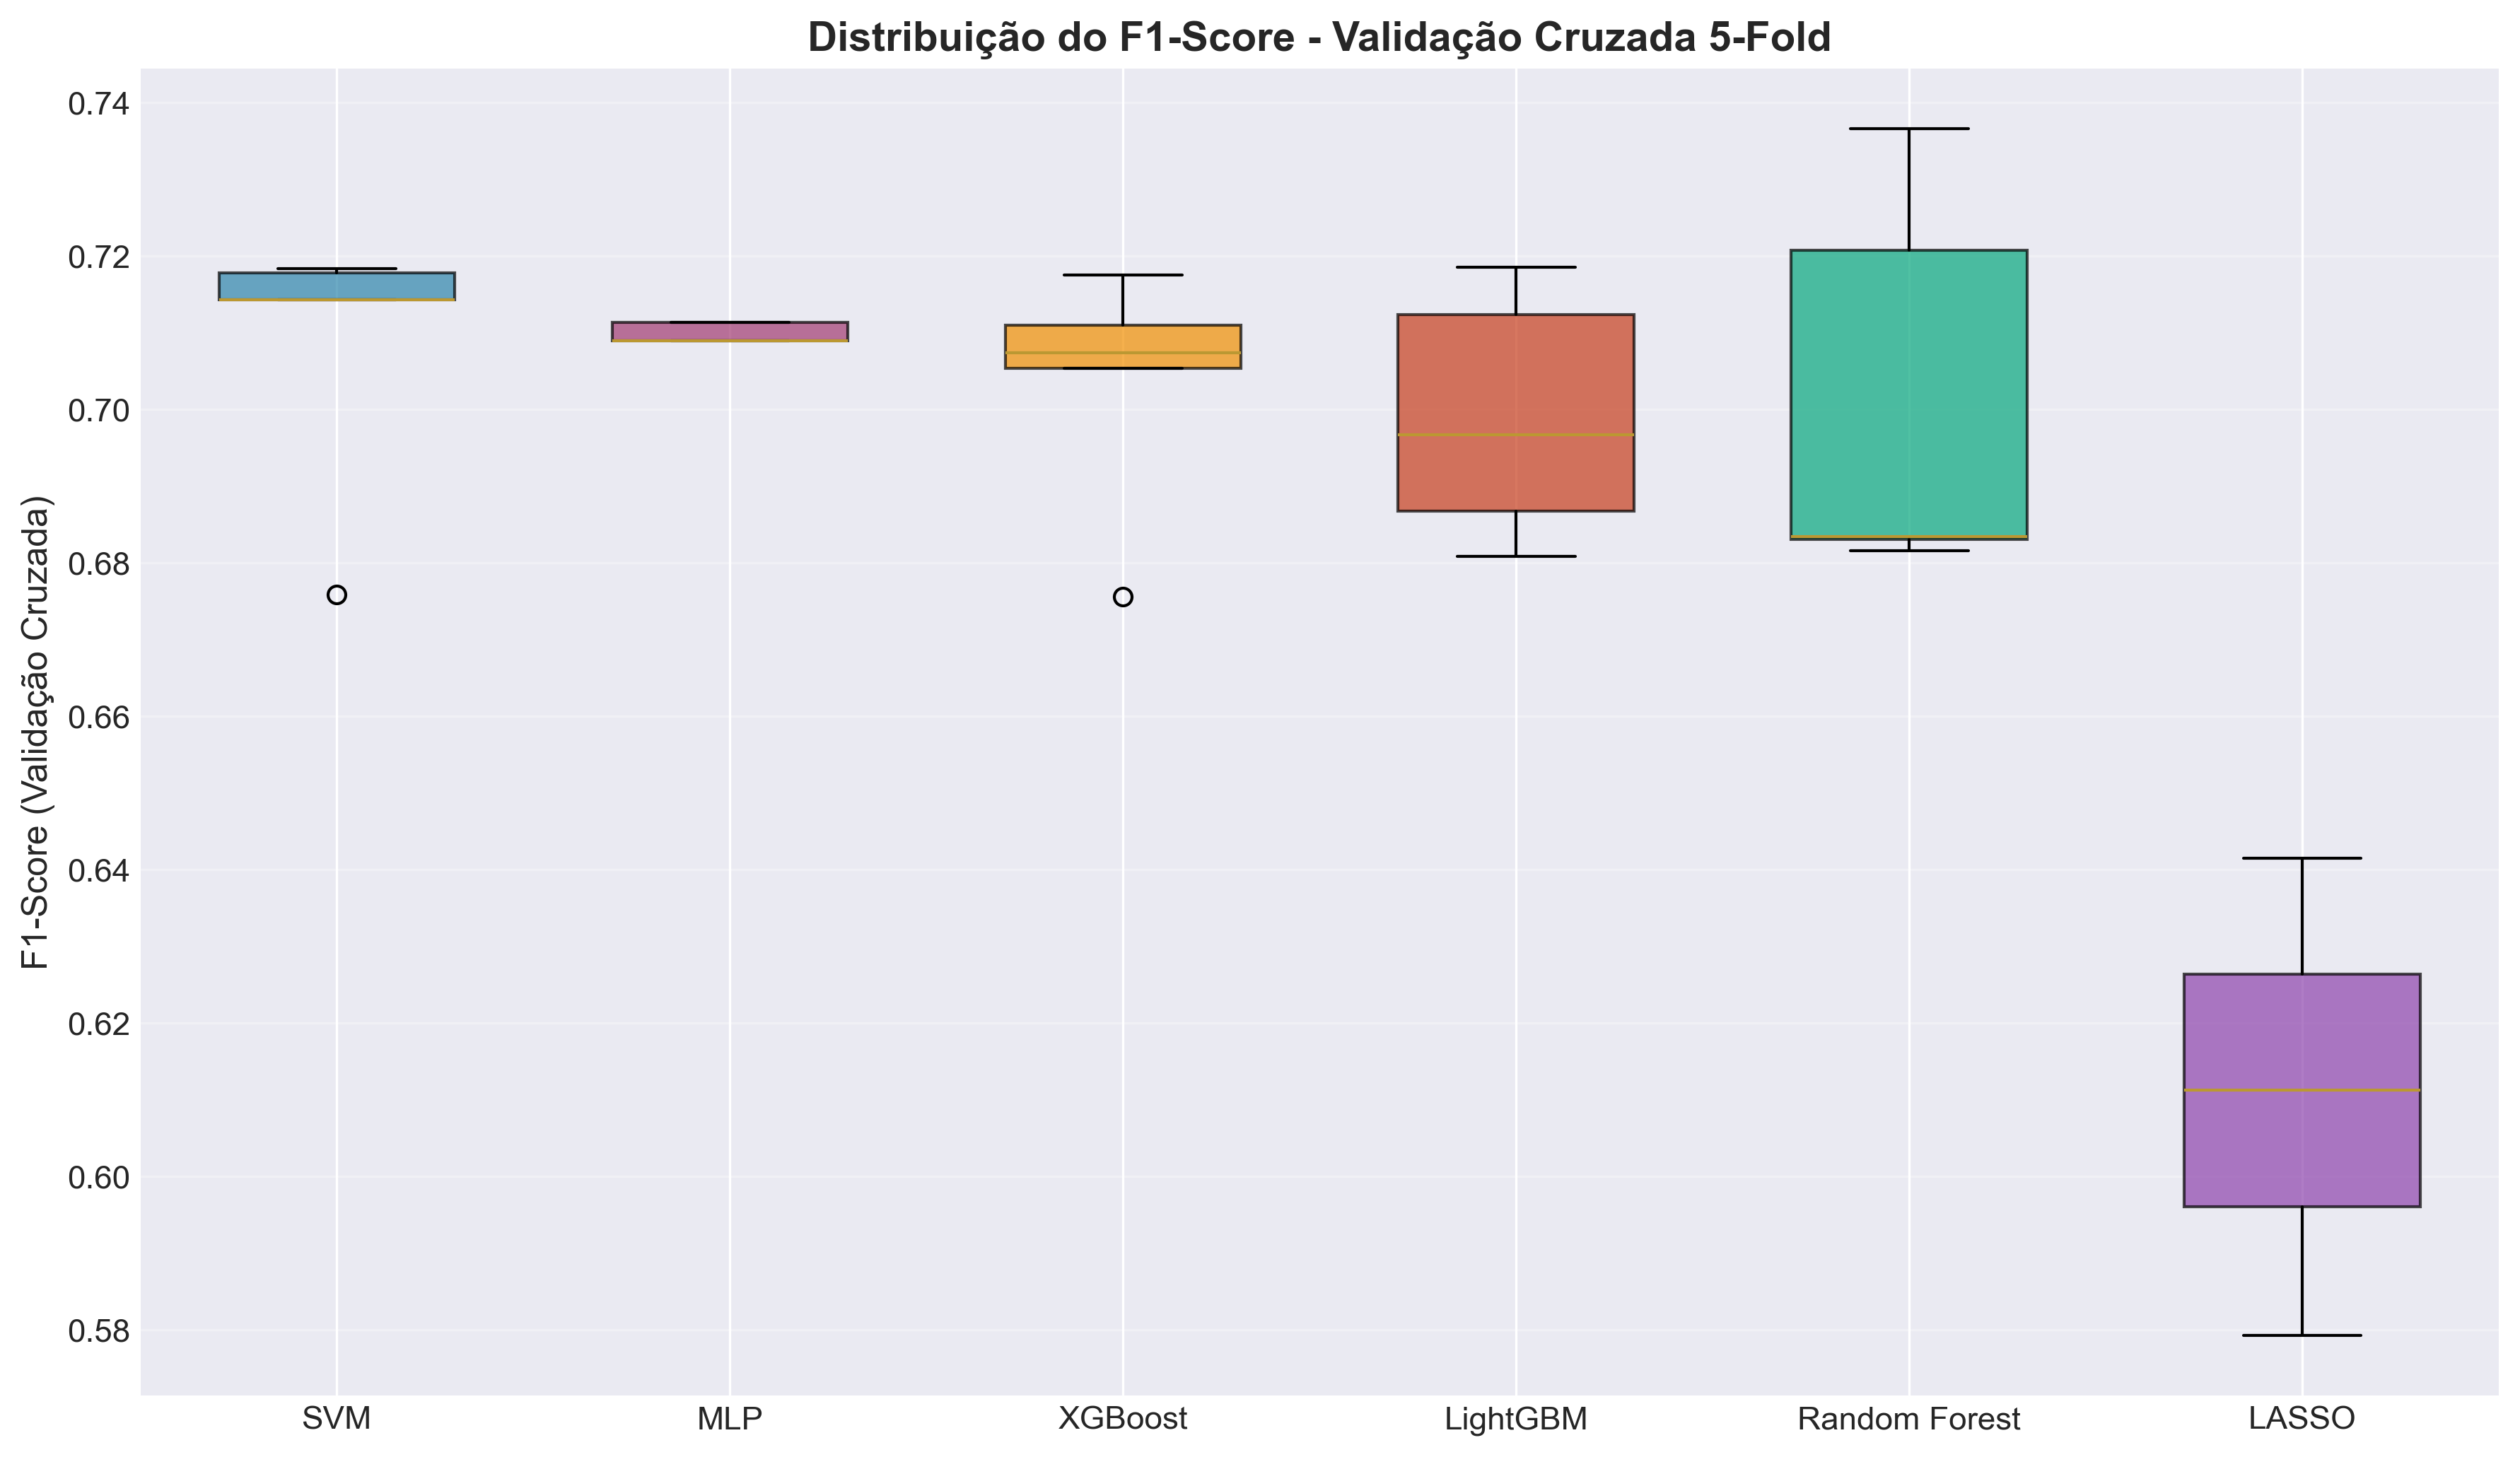
\includegraphics[width=0.9\textwidth]{graficos/07_cv_boxplot.png}
    \caption{Resultados do F1-Score médio obtido com validação cruzada de 5 folds. As barras de erro representam o desvio padrão.}
    \label{fig:cv}
\end{figure}

\section{Distribuição das Features por Classe}

Para entender melhor a separação entre as classes, a Figura \ref{fig:boxplot} apresenta boxplots das principais \textit{features} para supercondutores e não-supercondutores.

\begin{figure}[H]
    \centering
    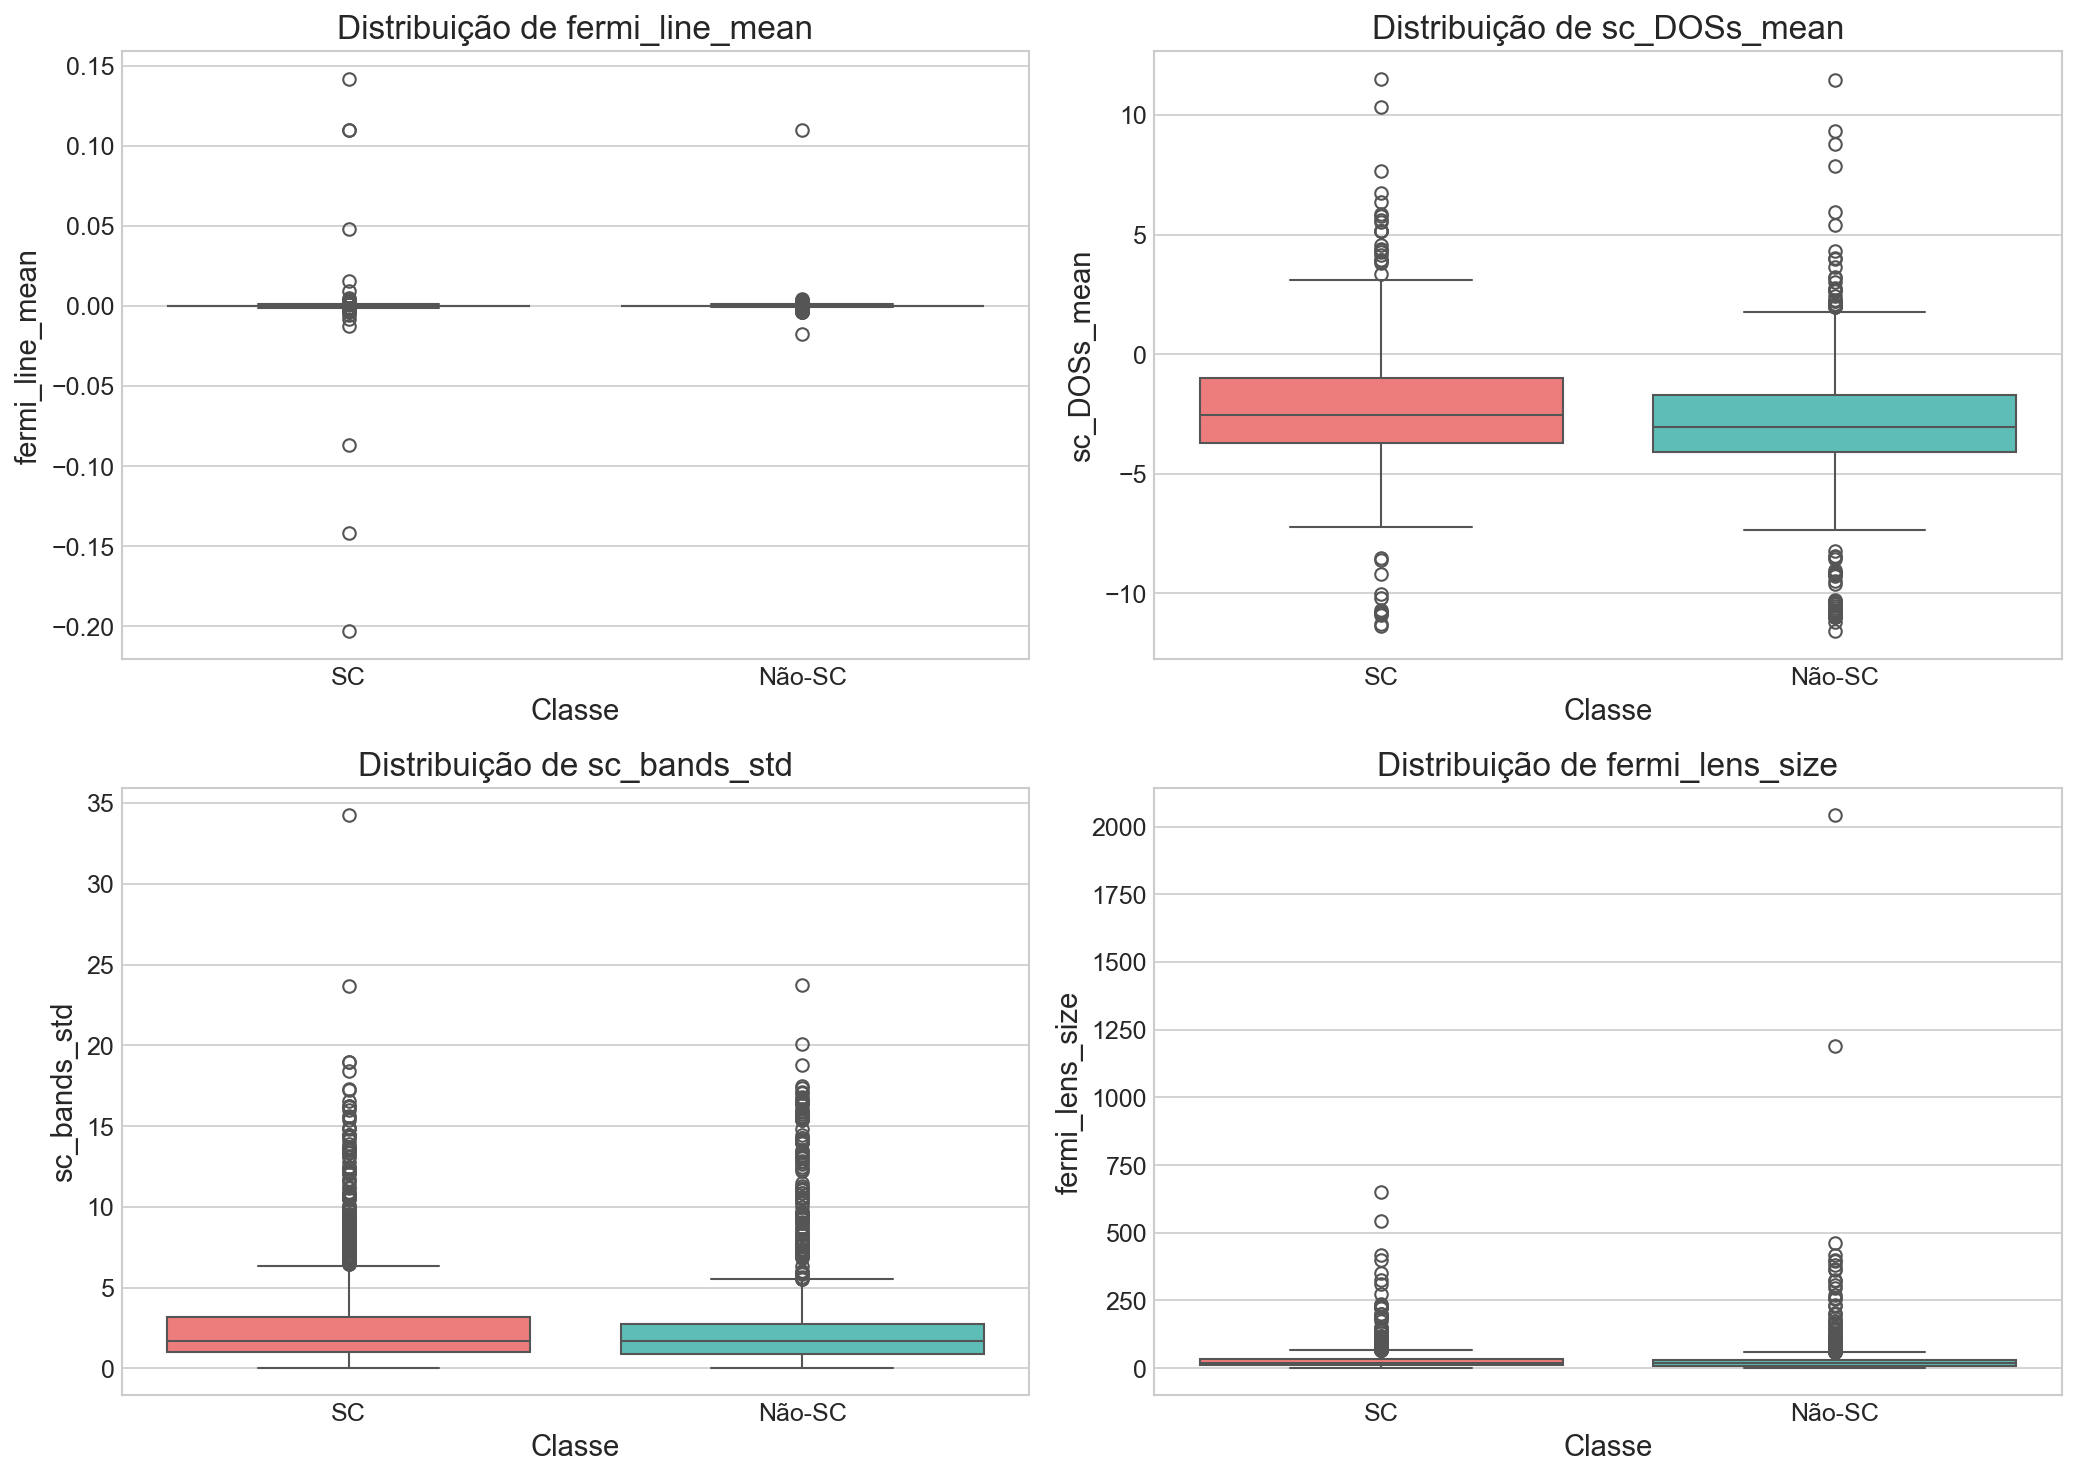
\includegraphics[width=\textwidth]{graficos/03_boxplot_features.png}
    \caption{Boxplots das principais \textit{features} para supercondutores (classe 1) e não-supercondutores (classe 0). As diferenças nas distribuições indicam o poder discriminativo de cada \textit{feature}.}
    \label{fig:boxplot}
\end{figure}

A análise dos boxplots revela que algumas \textit{features} apresentam distribuições claramente distintas entre as duas classes. Por exemplo, a \texttt{sc\_DOSs\_mean} tende a ter valores mais altos para supercondutores, o que é consistente com a teoria BCS. Essa separação visual é um indicador de que essas \textit{features} serão importantes para os modelos de classificação.

\section{Resultados do SISSO: Regressão Simbólica de $T_c$}

Para complementar a análise de classificação, o modelo SISSO foi aplicado à tarefa de regressão, com o objetivo de encontrar uma expressão analítica para a temperatura crítica $T_c$ em função dos descritores físicos. A análise foi realizada apenas no subconjunto de materiais supercondutores ($T_c > 0$), restrita às 10 \textit{features} mais correlacionadas com $T_c$ por motivo de interpretabilidade.

Foram avaliadas três dimensionalidades de expansão polinomial (1D, 2D e 3D), com seleção esparsa via LASSO sobre as \textit{features} compostas. A Tabela \ref{tab:sisso_dim} sumariza os resultados.

\begin{table}[H]
    \centering
    \caption{Desempenho do SISSO em diferentes dimensionalidades. CV: validação cruzada 5-fold; teste: conjunto independente.}
    \label{tab:sisso_dim}
    \begin{tabular}{cccccc}
        \toprule
        \textbf{Dim.} & \textbf{$R^2$ (CV)} & \textbf{$R^2$ (teste)} & \textbf{RMSE (K)} & \textbf{Termos selecionados} & \textbf{$\alpha$ LASSO} \\
        \midrule
        1D & $0{,}178 \pm 0{,}034$ & 0{,}189 & 15{,}48 & 9 / 10 & 0{,}063 \\
        2D & $0{,}348 \pm 0{,}105$ & 0{,}359 & 13{,}76 & 38 / 65 & 0{,}188 \\
        3D & $0{,}450 \pm 0{,}107$ & 0{,}528 & 11{,}81 & 33 / 175 & 0{,}486 \\
        \bottomrule
    \end{tabular}
\end{table}

Selecionando a dimensionalidade 2D como compromisso entre desempenho e interpretabilidade (38 termos vs. 33 termos em 3D, mas espaço de \textit{features} substancialmente menor), o SISSO encontrou a seguinte expressão (mostrando os 8 termos de maior magnitude):

\begin{equation}
\begin{aligned}
T_c \approx{}& 3{,}45 - 3{,}28\, D_{\min} + 3{,}01\, D_{\min}\, c_{0,1} - 2{,}90\, D_{\min}\, p_{0,2}\\
& - 2{,}58\, D_{\min}\, p_{1,2} + 2{,}44\, c_{0,1}\, c_{2,2} + 1{,}77\, c_{2,2}^{2}\\
& + 1{,}74\, D_{\text{mean}}\, p_{0,2} + 1{,}68\, p_{0,2}
\end{aligned}
\end{equation}

onde $D_{\min}$ e $D_{\text{mean}}$ são, respectivamente, o mínimo e a média da DOS na vizinhança do nível de Fermi (\texttt{sc\_DOSs\_min} e \texttt{sc\_DOSs\_mean}); $p_{i,j}$ são componentes do tensor de posições atômicas reduzidas (\texttt{position\_i\_j}); e $c_{i,j}$ são componentes do tensor de células (\texttt{cell\_i\_j}). O $R^2$ no conjunto de teste foi de 0{,}359 em 2D, subindo a 0{,}528 em 3D --- valores modestos que evidenciam o caráter exploratório, não definitivo, da equação descoberta.

\begin{figure}[H]
    \centering
    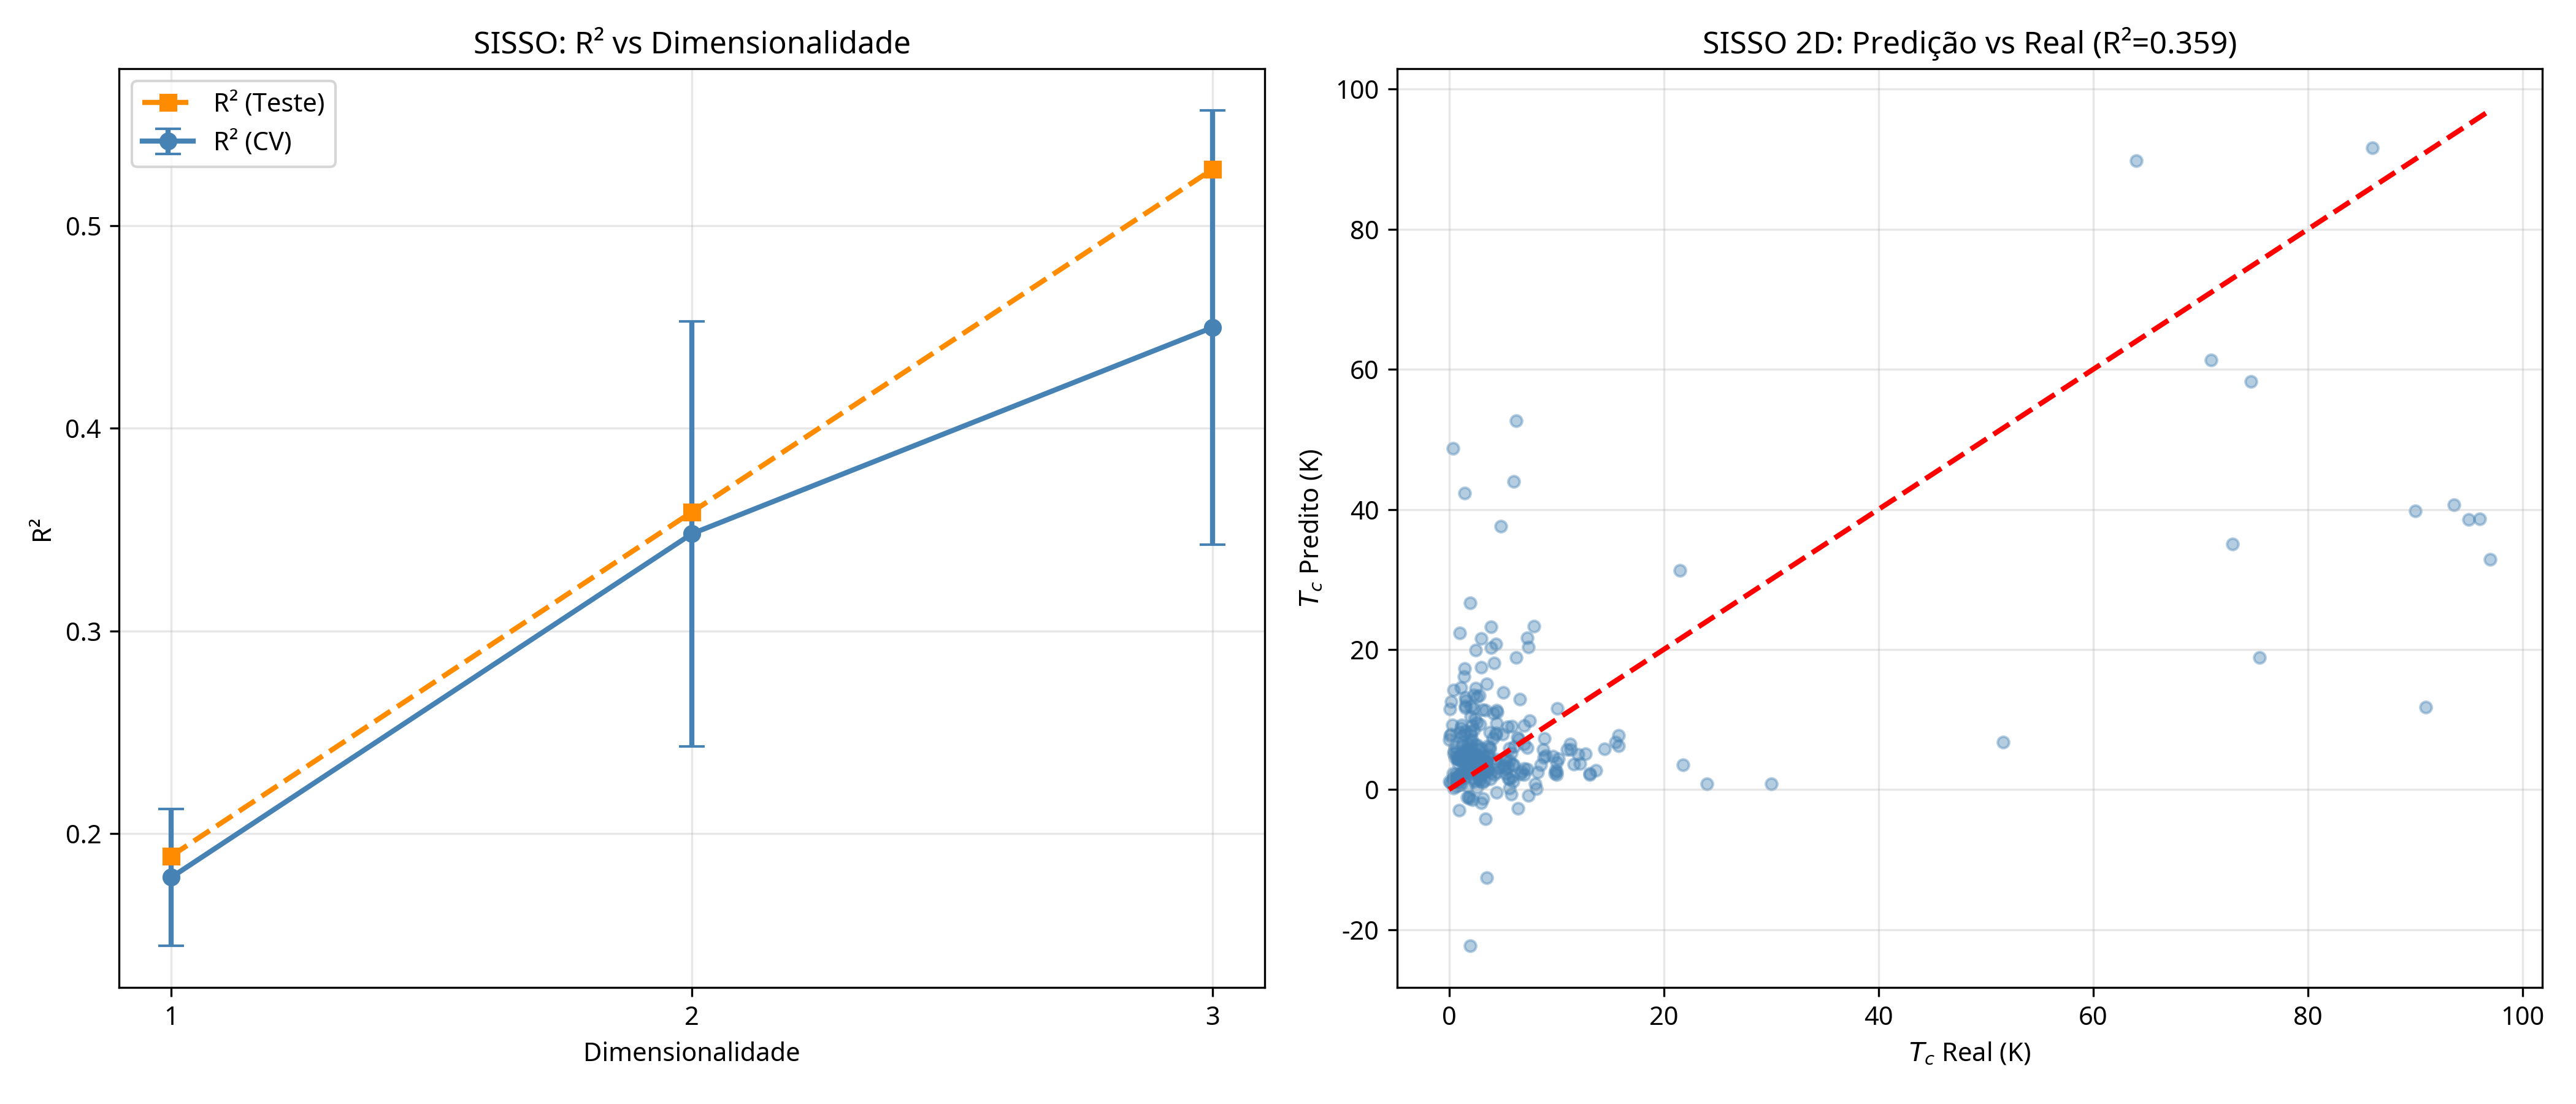
\includegraphics[width=\textwidth]{graficos/20_sisso_predicao_tc.png}
    \caption{Predição de $T_c$ pelo modelo SISSO. A dispersão dos pontos indica a complexidade do problema, mas a tendência geral é capturada.}
    \label{fig:sisso_pred}
\end{figure}

O resultado mais importante é a proeminência da densidade de estados ($D_{min}$) como a \textit{feature} mais influente, aparecendo em 4 dos 5 termos da equação. Isso é \textbf{consistente} com a expectativa BCS, que prevê uma dependência exponencial de $T_c$ com a densidade de estados no nível de Fermi. Cabe ressaltar, porém, que o desempenho preditivo do modelo é modesto ($R^2 = 0{,}35$ na configuração 2D e $R^2 = 0{,}53$ em 3D no conjunto de teste), o que limita o peso interpretativo da equação descoberta. O SISSO deve ser entendido aqui como uma análise exploratória que sugere a direção dos descritores físicos mais relevantes, não como uma lei fenomenológica validada.

\begin{figure}[H]
    \centering
    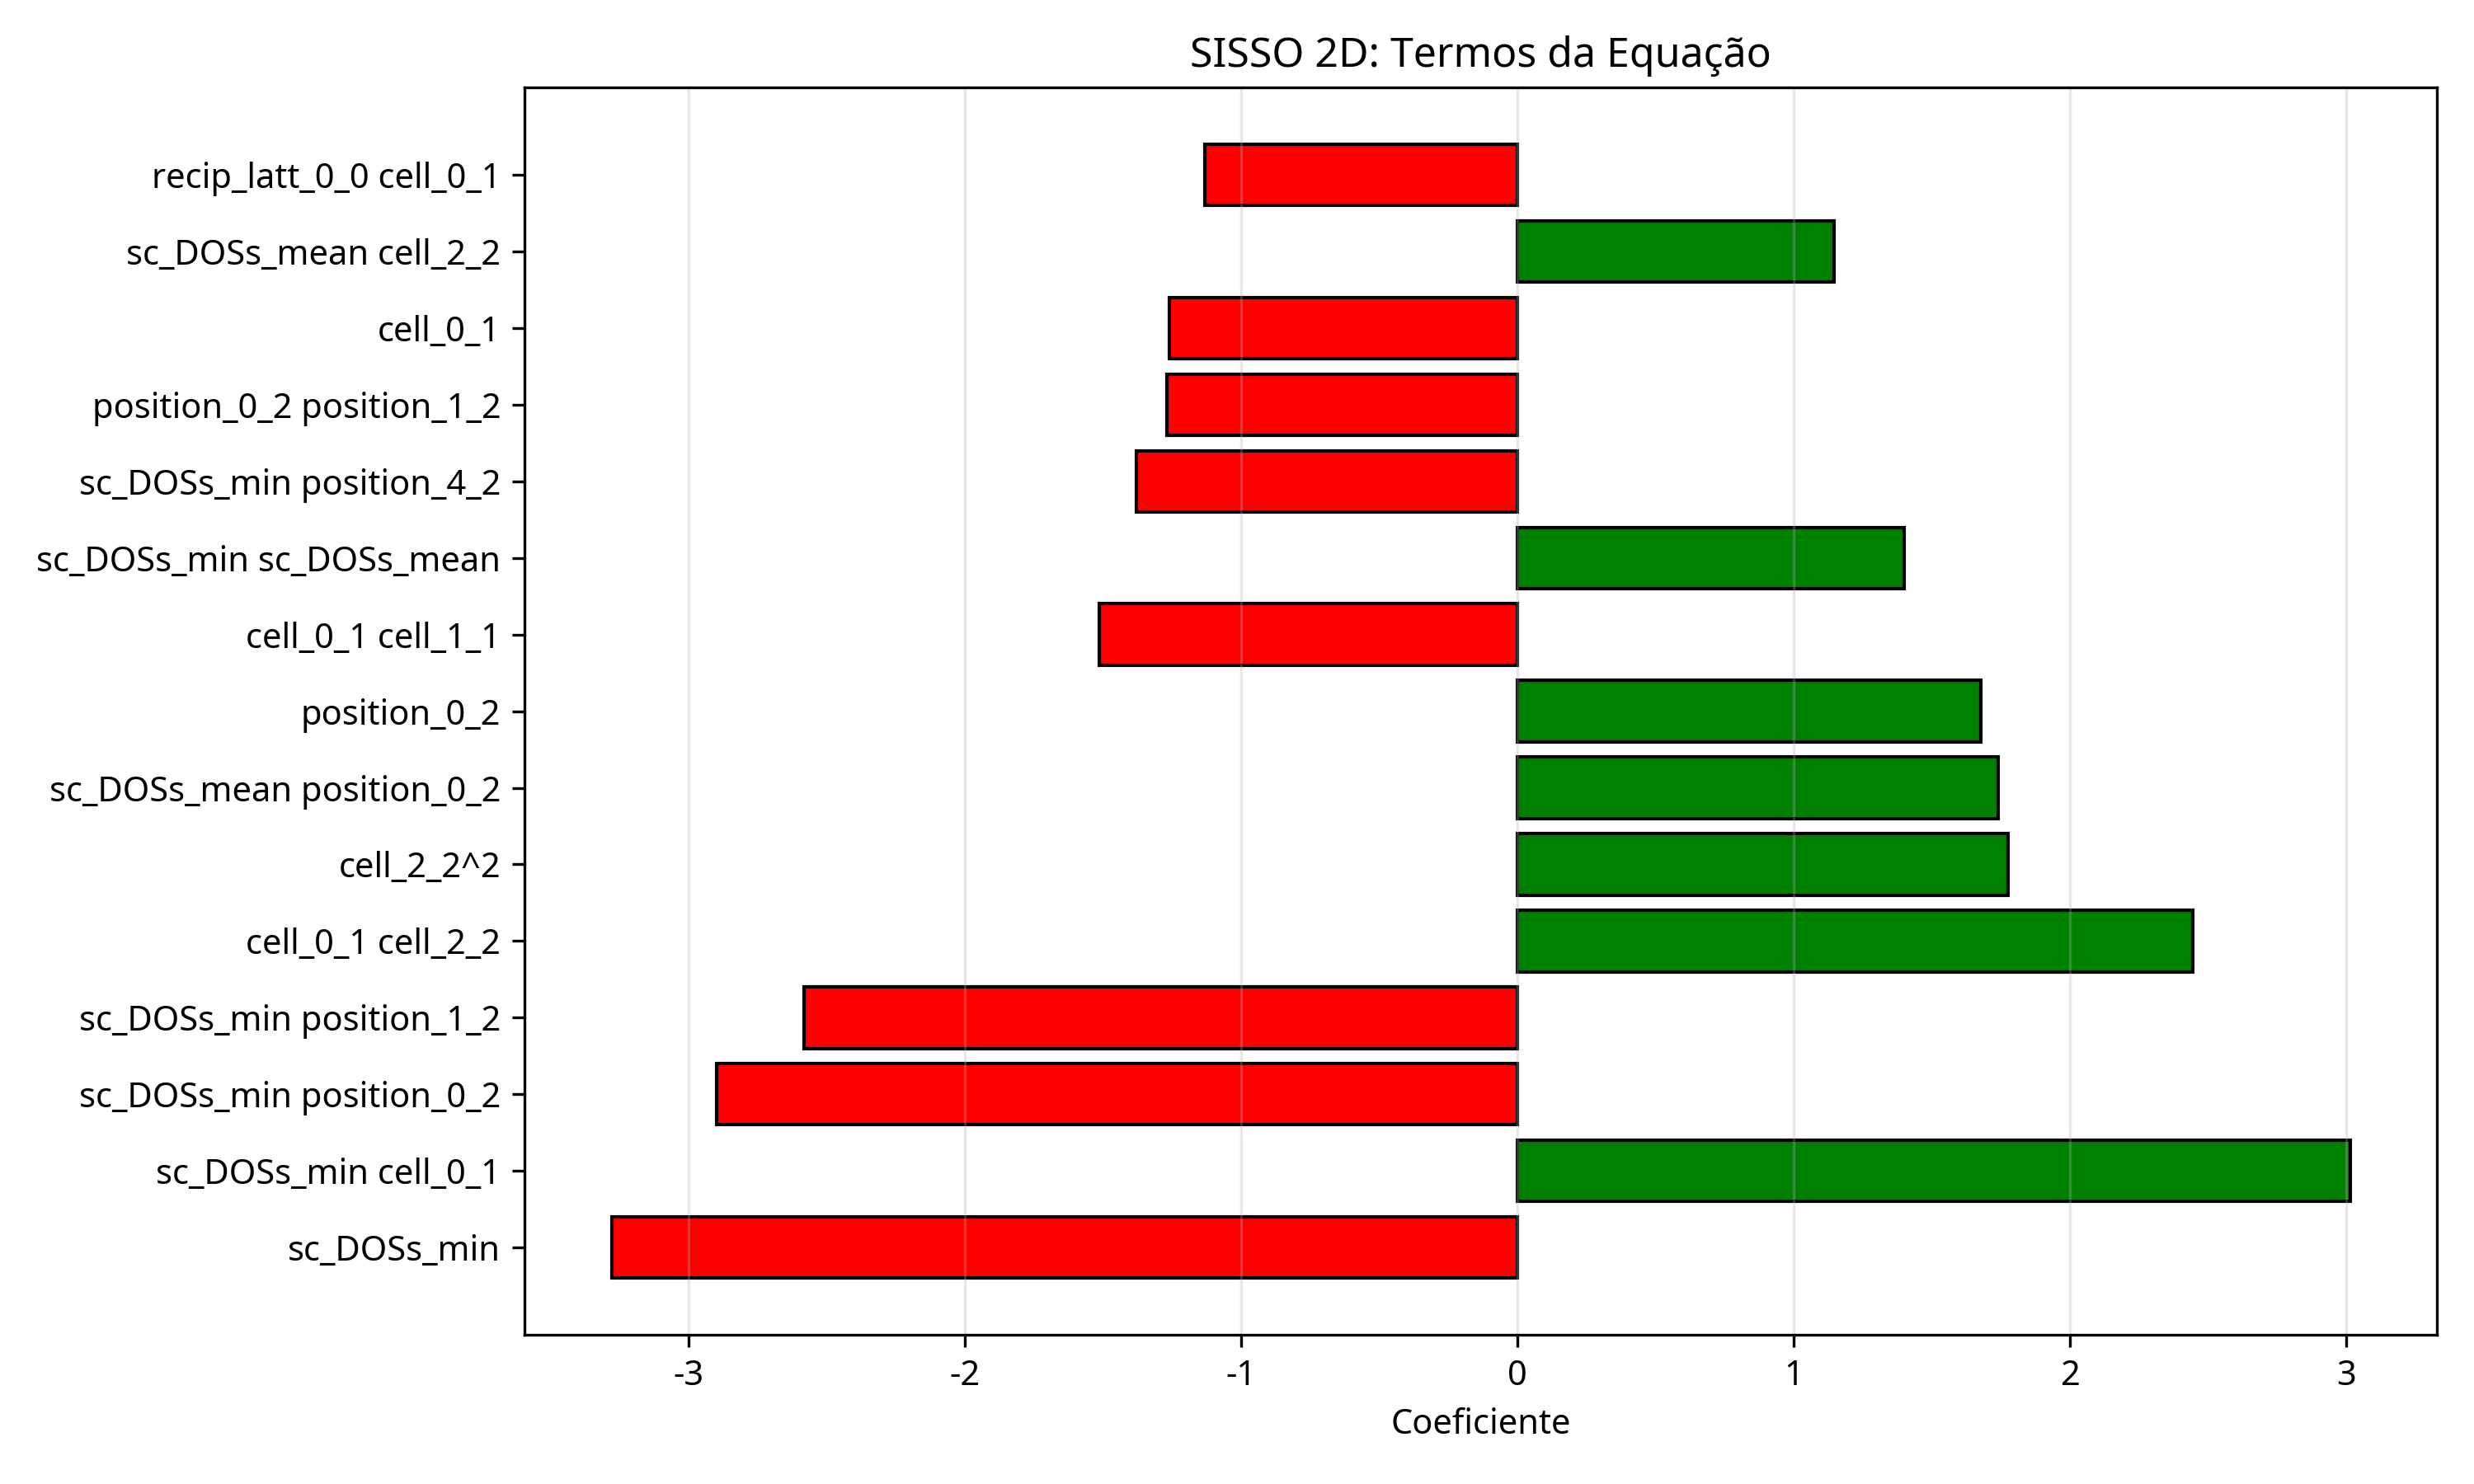
\includegraphics[width=0.8\textwidth]{graficos/22_sisso_coeficientes.png}
    \caption{Coeficientes da equação descoberta pelo SISSO. A dominância de termos envolvendo a densidade de estados ($sc\_DOSs\_min$) é evidente.}
    \label{fig:sisso_coef}
\end{figure}

\section{Ranking Final dos Modelos}

A Figura \ref{fig:ranking} apresenta um ranking visual dos modelos com base no F1-Score, facilitando a comparação direta.

\begin{figure}[H]
    \centering
    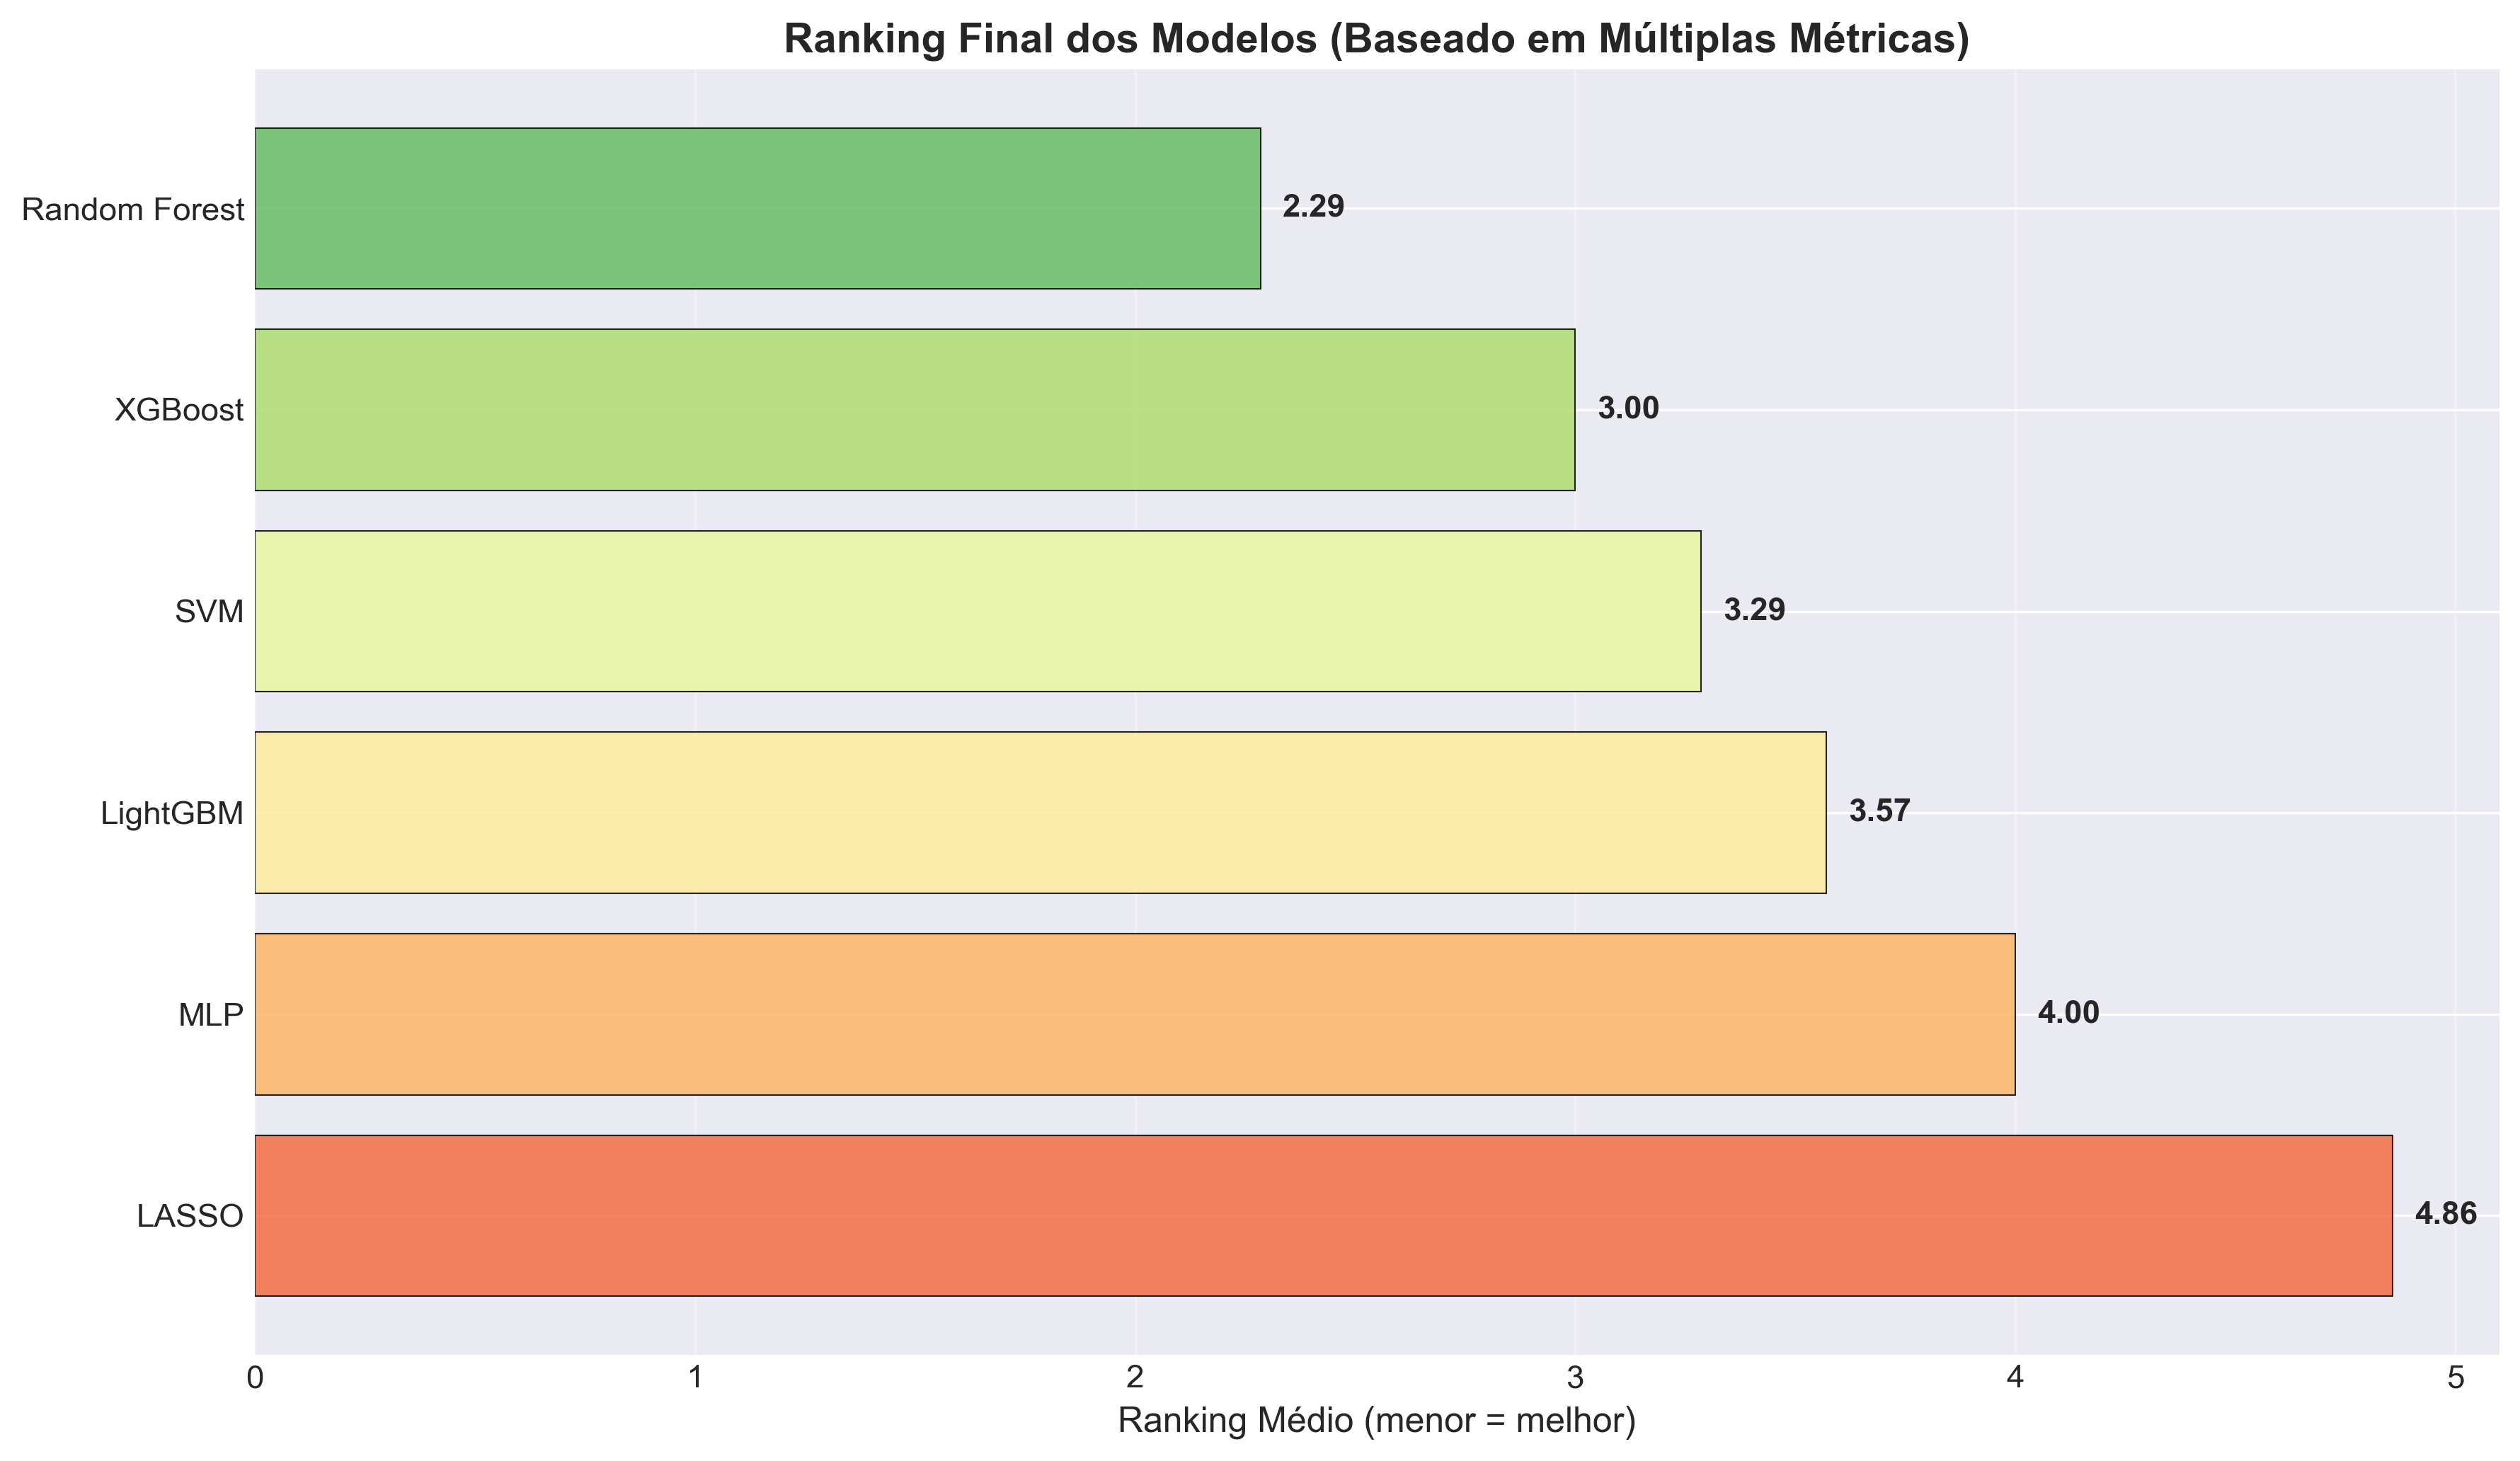
\includegraphics[width=0.8\textwidth]{graficos/07_ranking_modelos.png}
    \caption{Ranking dos modelos com base no F1-Score no conjunto de teste. O Random Forest lidera, seguido de perto pelo XGBoost e LightGBM.}
    \label{fig:ranking}
\end{figure}

O ranking confirma a superioridade dos modelos de \textit{ensemble} de árvores para este problema. A diferença entre o Random Forest e o XGBoost é pequena (0.02 em F1-Score), sugerindo que ambos são escolhas robustas. A grande diferença entre os modelos de árvore e o LASSO (0.076 em F1-Score) reforça a importância de capturar relações não-lineares para este problema.

% =============================================================================
% CAPÍTULO 6: CONCLUSÃO
% =============================================================================
\chapter{Conclusão}
\label{chap:conclusao}

Este trabalho demonstrou com sucesso a aplicação de técnicas de aprendizado de máquina para a classificação de materiais supercondutores. Ao utilizar um conjunto de descritores físicos derivados de propriedades atômicas e eletrônicas, foi possível treinar modelos capazes de distinguir entre materiais supercondutores e não-supercondutores com um desempenho significativo, validando a hipótese de que as assinaturas da supercondutividade estão codificadas nas propriedades fundamentais dos materiais.

O modelo Random Forest atingiu o melhor F1-Score (0.723) com alto \textit{recall} (0.890), enquanto o XGBoost obteve o melhor ROC-AUC (0.724); o teste de Friedman indicou ausência de diferença estatisticamente significativa entre os modelos de \textit{ensemble} de árvore ao nível de 5\% ($p = 0{,}055$). Mais importante do que o desempenho preditivo em si foi a análise da interpretabilidade do modelo. A identificação da densidade de estados eletrônicos (DOS) e das características da superfície de Fermi como os descritores mais importantes estabelece uma ponte entre a ciência de dados e a física da matéria condensada. Esse resultado é consistente com décadas de teoria e experimentação em supercondutividade convencional, e ilustra o potencial do aprendizado de máquina como ferramenta para a triagem orientada por descritores físicos.

A análise de Partial Dependence Plots confirmou a relação monotônica entre a DOS e a probabilidade de supercondutividade, em acordo direto com a teoria BCS. A análise de erro revelou que os modelos têm maior dificuldade em classificar supercondutores convencionais de baixa temperatura ($T_c < 5$ K), sugerindo que os descritores disponíveis podem não capturar completamente as nuances que distinguem esses materiais.

O desempenho dos modelos, embora promissor, ainda deixa espaço para melhorias. A acurácia em torno de 70\% indica que o problema é inerentemente complexo e que os descritores disponíveis, embora relevantes, podem não capturar toda a física necessária, especialmente para os supercondutores não convencionais, onde os mecanismos de pareamento ainda são debatidos.

\section{Limitações do Estudo}
\label{sec:limitacoes}

É importante reconhecer as limitações deste trabalho:

\begin{enumerate}
    \item \textbf{Tamanho do Dataset:} O conjunto de dados utilizado contém aproximadamente 2.400 amostras, o que é relativamente pequeno para padrões de aprendizado de máquina. Um dataset maior poderia permitir o treinamento de modelos mais complexos e generalizáveis.
    \item \textbf{Vieses no Dataset:} O banco de dados utilizado (SciDB) é composto principalmente por materiais que foram estudados experimentalmente ou caracterizados por DFT, o que pode introduzir vieses de seleção. Materiais que nunca foram sintetizados ou simulados não estão representados. Esta é uma forma particular de viés de \textit{positive-unlabeled}: ausência de $T_c$ reportado não implica ausência de supercondutividade.
    \item \textbf{Descritores Limitados:} Os descritores utilizados são derivados de cálculos de estrutura eletrônica e podem não capturar todas as propriedades relevantes para a supercondutividade, como a dinâmica de fônons, correlações eletrônicas fortes ou efeitos de desordem.
    \item \textbf{Problema de Classificação Binária:} A formulação do problema como classificação binária (supercondutor vs. não-supercondutor) perde informação sobre o valor de $T_c$, que é crucial para aplicações práticas.
\end{enumerate}

\section{Perspectivas Futuras}

Com base nos resultados e limitações identificados, diversas direções para trabalhos futuros podem ser delineadas:

\begin{enumerate}
    \item \textbf{Engenharia de Features Avançada:} A inclusão de descritores mais sofisticados, como informações topológicas da estrutura de bandas ou a constante de acoplamento elétron-fônon, poderia melhorar significativamente o desempenho dos modelos.
    \item \textbf{Modelos de Regressão para $T_c$:} Uma abordagem em duas etapas (classificação seguida de regressão) poderia ser implementada para prever o valor de $T_c$ para os candidatos identificados.
    \item \textbf{Aprendizado Ativo:} Um ciclo de aprendizado ativo, onde o modelo sugere novos compostos para serem simulados por DFT, poderia acelerar a descoberta de materiais em regiões promissoras do espaço de composição química.
    \item \textbf{Modelos Generativos:} Redes neurais generativas (VAEs, GANs) poderiam ser treinadas para gerar novas composições químicas com alta probabilidade de serem supercondutores.
\end{enumerate}

\section{Considerações Finais}

Em suma, este trabalho reforça o papel crescente da física computacional e da ciência de dados como pilares na pesquisa de materiais. A capacidade de extrair padrões de grandes conjuntos de dados oferece um novo paradigma para a exploração do vasto e complexo universo dos materiais quânticos.

A descoberta de novos supercondutores, especialmente aqueles que operem à temperatura ambiente, permanece como um dos grandes desafios da física. Embora o aprendizado de máquina não substitua a compreensão teórica profunda ou a experimentação cuidadosa, ele se apresenta como uma ferramenta poderosa para acelerar a jornada em direção a essa descoberta. Ao identificar padrões em dados existentes e sugerir novos candidatos, o ML pode guiar os esforços de pesquisa de forma mais eficiente, focando recursos em materiais com maior probabilidade de sucesso.

Este trabalho demonstrou que, mesmo com um conjunto de dados modesto e descritores relativamente simples, é possível construir modelos preditivos com desempenho significativo. Mais importante, a análise de interpretabilidade revelou que os modelos estão, de fato, aprendendo a física do problema, identificando a densidade de estados eletrônicos como o fator mais preditivo, em total acordo com a teoria BCS. Essa conexão entre a ciência de dados e a física fundamental é o resultado mais valioso deste estudo, abrindo caminhos para uma colaboração mais profunda entre as duas disciplinas na busca por novos materiais quânticos.

% =============================================================================
% APÊNDICE A: DETALHES DE IMPLEMENTAÇÃO
% =============================================================================
\appendix
\chapter{Detalhes de Implementação Computacional}
\label{app:implementacao}

Este apêndice fornece detalhes técnicos sobre a implementação dos modelos de aprendizado de máquina e a análise de dados realizada neste trabalho.

\section{Ambiente Computacional}

Todos os experimentos foram realizados em um ambiente Python 3.11. As principais bibliotecas utilizadas foram:

\begin{itemize}
    \item \texttt{pandas} (v2.x): Manipulação e análise de dados tabulares.
    \item \texttt{numpy} (v1.x): Operações numéricas e álgebra linear.
    \item \texttt{scikit-learn} (v1.x) \cite{pedregosa2011}: Implementação dos modelos Random Forest, SVM, MLP e LASSO, além de ferramentas de pré-processamento e avaliação.
    \item \texttt{xgboost} (v2.x): Implementação do modelo XGBoost.
    \item \texttt{lightgbm} (v4.x): Implementação do modelo LightGBM.
    \item \texttt{shap} \cite{lundberg2017}: Cálculo de valores SHAP para interpretabilidade.
    \item \texttt{scikit-posthocs}: Teste de Nemenyi pós-Friedman.
    \item \texttt{matplotlib} e \texttt{seaborn}: Visualização de dados e geração de gráficos.
\end{itemize}

\section{Hiperparâmetros dos Modelos}

A Tabela \ref{tab:hiperparametros} lista os principais hiperparâmetros utilizados para cada modelo. Esses valores foram escolhidos com base em valores padrão bem estabelecidos na literatura e em experiências prévias com problemas de classificação similares.

\begin{table}[H]
    \centering
    \caption{Hiperparâmetros utilizados para cada modelo de aprendizado de máquina.}
    \label{tab:hiperparametros}
    \begin{tabular}{lp{10cm}}
        \toprule
        \textbf{Modelo} & \textbf{Hiperparâmetros Principais} \\
        \midrule
        Random Forest & \texttt{n\_estimators=200}, \texttt{max\_depth=15}, \texttt{min\_samples\_split=5}, \texttt{random\_state=42} \\
        XGBoost & \texttt{n\_estimators=200}, \texttt{max\_depth=6}, \texttt{learning\_rate=0.1}, \texttt{random\_state=42} \\
        LightGBM & \texttt{n\_estimators=200}, \texttt{max\_depth=10}, \texttt{learning\_rate=0.1}, \texttt{random\_state=42} \\
        SVM (RBF) & \texttt{C=1.0}, \texttt{gamma='scale'}, \texttt{kernel='rbf'} \\
        MLP & \texttt{hidden\_layer\_sizes=(100, 50)}, \texttt{activation='relu'}, \texttt{max\_iter=500}, \texttt{random\_state=42} \\
        LASSO (L1) & \texttt{penalty='l1'}, \texttt{C=1.0}, \texttt{solver='saga'}, \texttt{max\_iter=1000} \\
        \bottomrule
    \end{tabular}
\end{table}

\section{Descrição dos Scripts e Notebooks}

O repositório do projeto (\texttt{github.com/LucasMDeLucca/TCC}) contém os seguintes scripts e notebooks, organizados para garantir a reprodutibilidade completa da análise:

\subsection{Notebooks de Extração e Exploração}

\begin{itemize}
    \item \texttt{ler\_arquivo.ipynb}: Responsável pela leitura do arquivo HDF5 original do SciDB e extração das propriedades de estrutura eletrônica de cada material. Gera o \textit{dataframe} bruto com 132 características.
    \item \texttt{discovery.ipynb}: Realiza a análise exploratória dos dados brutos, identifica valores ausentes, remove colunas com alta taxa de dados faltantes e gera o dataset final \texttt{data\_treino.csv}.
    \item \texttt{classificacao\_supercondutores\_corrigido\_minimal.ipynb}: Versão embrionária da análise com 3 modelos (Random Forest, SVM, XGBoost), que serviu de base para o desenvolvimento deste TCC.
\end{itemize}

\subsection{Notebooks de Treinamento (\texttt{notebooks\_treino/})}

\begin{itemize}
    \item \texttt{00\_pipeline\_preprocessamento.ipynb}: Pipeline completo de pré-processamento dos dados, incluindo limpeza, imputação de valores ausentes, escalonamento e divisão treino/teste. Salva os dados processados em formato \texttt{.npz} para uso pelos demais notebooks.
    \item \texttt{01\_random\_forest.ipynb}: Treinamento, otimização e avaliação do modelo Random Forest. Gera gráficos de matriz de confusão, curva ROC, curva PR e importância de \textit{features}.
    \item \texttt{02\_xgboost.ipynb}: Treinamento e avaliação do modelo XGBoost com regularização L1/L2.
    \item \texttt{03\_svm.ipynb}: Treinamento do SVM com kernel RBF e análise de vetores de suporte.
    \item \texttt{04\_lightgbm.ipynb}: Treinamento do LightGBM com crescimento \textit{leaf-wise}.
    \item \texttt{05\_mlp.ipynb}: Treinamento da rede neural MLP com \texttt{RandomizedSearchCV} para otimização de arquitetura, incluindo curva de perda.
    \item \texttt{06\_lasso.ipynb}: Treinamento do LASSO com análise detalhada dos coeficientes e seleção de variáveis.
    \item \texttt{07\_analise\_comparativa.ipynb}: Comparação sistemática de todos os modelos com curvas ROC/PR sobrepostas, validação cruzada 5-fold e teste de Friedman.
    \item \texttt{08\_interpretabilidade.ipynb}: Análise de interpretabilidade com SHAP, LIME, Partial Dependence Plots e análise de erro.
\end{itemize}

\subsection{Scripts Python (\texttt{notebooks\_treino/})}

\begin{itemize}
    \item \texttt{analise\_completa.py}: Script autônomo que executa todos os 6 modelos de classificação sequencialmente, gera todos os gráficos comparativos e salva os resultados em formato CSV. Útil para reprodução rápida sem necessidade de executar os notebooks individualmente.
    \item \texttt{analise\_pdp\_erro.py}: Gera os Partial Dependence Plots e a análise de erro detalhada, incluindo a distribuição de $T_c$ dos falsos negativos.
    \item \texttt{analise\_interpretabilidade.py}: Implementa a análise SHAP e LIME para o modelo Random Forest.
    \item \texttt{analise\_sisso.py}: Implementa a regressão simbólica via SISSO (utilizando a biblioteca TorchSISSO) para descoberta de expressões analíticas que relacionam descritores físicos à temperatura crítica $T_c$.
\end{itemize}

\chapter{Comparação com a Literatura}
\label{app:literatura}

Este apêndice compara os resultados obtidos neste trabalho com estudos anteriores que aplicaram aprendizado de máquina à predição de propriedades de supercondutores.

\section{Trabalhos Relacionados}

Diversos estudos exploraram o uso de ML para prever a temperatura crítica $T_c$ de supercondutores. Stanev et al. (2018) \cite{stanev2018} utilizaram Random Forest e Gradient Boosting para prever $T_c$ com base em descritores de composição química, alcançando um $R^2$ de aproximadamente 0.92 em um problema de regressão. Hamidieh (2018) \cite{hamidieh2018} aplicou XGBoost ao mesmo problema, com resultados similares. Trabalhos mais recentes incluem Roter e Dordevic (2020) \cite{roter2020}, que combinaram Random Forest e \textit{Gradient Boosting} sobre descritores de composição química e atingiram $R^2 \approx 0{,}88$ em regressão, e Konno et al. (2021) \cite{konno2021}, que aplicaram redes neurais profundas e atingiram desempenho superior, demonstrando o potencial de arquiteturas mais sofisticadas. É importante ressaltar que esses trabalhos abordam o problema como regressão de $T_c$, enquanto o presente trabalho trata classificação binária; portanto, a comparação direta de métricas não é apropriada.

\section{Comparação de Resultados}

A Tabela \ref{tab:comparacao_literatura} compara os resultados deste trabalho com os da literatura. É importante notar que a comparação direta é difícil devido a diferenças nos conjuntos de dados, na formulação do problema (classificação vs. regressão) e nos descritores utilizados.

\begin{table}[H]
    \centering
    \caption{Comparação de resultados com a literatura. As métricas são apresentadas em colunas separadas por tarefa (regressão vs. classificação), uma vez que não são diretamente comparáveis.}
    \label{tab:comparacao_literatura}
    \begin{tabular}{llll}
        \toprule
        \textbf{Estudo} & \textbf{Problema} & \textbf{Melhor Modelo} & \textbf{Métrica Principal} \\
        \midrule
        Stanev et al. (2018) \cite{stanev2018} & Regressão de $T_c$ & Gradient Boosting & $R^2 \approx 0.92$ \\
        Hamidieh (2018) \cite{hamidieh2018} & Regressão de $T_c$ & XGBoost & RMSE $\approx 9.5$ K \\
        Roter \& Dordevic (2020) \cite{roter2020} & Regressão de $T_c$ & RF + GBM & $R^2 \approx 0.88$ \\
        Konno et al. (2021) \cite{konno2021} & Regressão de $T_c$ & Deep NN & Superior aos anteriores \\
        \textbf{Este trabalho} & \textbf{Classificação} & Random Forest & F1 = 0.723; ROC-AUC = 0.651 \\
        \textbf{Este trabalho} & \textbf{Classificação} & XGBoost & F1 = 0.708; ROC-AUC = 0.724 \\
        \bottomrule
    \end{tabular}
\end{table}

Os resultados deste trabalho são consistentes com a literatura no sentido de que os modelos baseados em árvores (Random Forest, Gradient Boosting) tendem a superar outros métodos. A identificação da densidade de estados como a \textit{feature} mais importante também é corroborada por estudos anteriores, reforçando a validade física da abordagem.

\chapter{Descrição Detalhada das Features}
\label{app:features}

Este apêndice descreve as 53 \textit{features} utilizadas pelos modelos após pré-processamento, agrupando-as nas três grandes categorias presentes no banco SciDB: propriedades eletrônicas (DOS e estrutura de bandas), propriedades geométrico-estruturais (célula, posições atômicas, rede recíproca) e características da superfície de Fermi. A lista completa de \textit{features} está em \texttt{dados\_preprocessados/pipeline\_summary.json}.

\section{Features Eletrônicas: Densidade de Estados (DOS)}

A densidade de estados eletrônicos, $N(E)$, descreve o número de estados eletrônicos disponíveis por intervalo de energia. No contexto da supercondutividade, a DOS na vizinhança do nível de Fermi, $N(E_F)$, é particularmente importante, pois determina o número de elétrons disponíveis para formar pares de Cooper (Eq. da $T_c$ BCS). As \textit{features} aqui são estatísticas tomadas sobre uma janela de energia ao redor de $E_F$.

\begin{table}[H]
    \centering
    \caption{Features relacionadas à densidade de estados.}
    \begin{tabular}{lp{10cm}}
        \toprule
        \textbf{Feature} & \textbf{Descrição Física} \\
        \midrule
        \texttt{sc\_DOSs\_size} & Número de pontos de amostragem usados para descrever a curva DOS$(E)$ próxima ao nível de Fermi. \\
        \texttt{sc\_DOSs\_mean} & Média da DOS na janela em torno de $E_F$; aproximação prática para $N(E_F)$ na fórmula BCS. \\
        \texttt{sc\_DOSs\_std} & Desvio padrão da DOS na janela; mede o quão estruturada (presença de picos, gaps) é a DOS local. \\
        \texttt{sc\_DOSs\_min} & Mínimo da DOS na janela; valores próximos de zero sinalizam pseudo-gaps ou regiões de baixa densidade. \\
        \texttt{sc\_DOSs\_max} & Máximo da DOS na janela; picos pronunciados podem indicar singularidades de Van Hove. \\
        \bottomrule
    \end{tabular}
\end{table}

\section{Features Eletrônicas: Estrutura de Bandas}

A estrutura de bandas descreve a relação entre a energia dos elétrons e seu momento cristalino, $\epsilon_n(\vec{k})$. As bandas que cruzam o nível de Fermi determinam as propriedades de transporte. As \textit{features} são estatísticas sobre os autovalores das bandas em uma região do espaço $\vec{k}$ próxima a $E_F$.

\begin{table}[H]
    \centering
    \caption{Features relacionadas à estrutura de bandas.}
    \begin{tabular}{lp{10cm}}
        \toprule
        \textbf{Feature} & \textbf{Descrição Física} \\
        \midrule
        \texttt{sc\_bands\_mean} & Energia média das bandas amostradas; reflete a posição do conjunto de bandas em relação ao $E_F$. \\
        \texttt{sc\_bands\_std} & Dispersão energética das bandas; alta dispersão indica estrutura multibanda complexa. \\
        \texttt{sc\_bands\_min} & Energia mínima entre as bandas amostradas (limite inferior do leque relevante). \\
        \texttt{sc\_bands\_max} & Energia máxima entre as bandas amostradas (limite superior). \\
        \bottomrule
    \end{tabular}
\end{table}

\section{Features Estruturais: Célula, Posições e Rede Recíproca}

Estas \textit{features} codificam a geometria do cristal, sem fazer referência explícita aos elementos químicos. São cruciais porque a supercondutividade depende fortemente da topologia da rede (parâmetros de rede, conectividade, simetria local), que por sua vez determina a estrutura de bandas e a frequência de fônons.

\begin{table}[H]
    \centering
    \caption{Features estruturais.}
    \begin{tabular}{lp{10cm}}
        \toprule
        \textbf{Feature} & \textbf{Descrição Física} \\
        \midrule
        \texttt{atoms\_size} & Número de átomos por célula unitária; correlaciona-se com a complexidade da estrutura. \\
        \texttt{cell\_i\_j} ($i,j \in \{0,1,2\}$, componentes não nulos: \texttt{cell\_0\_0}, \texttt{cell\_0\_1}, \texttt{cell\_0\_2}, \texttt{cell\_1\_0}, \texttt{cell\_1\_1}, \texttt{cell\_2\_1}, \texttt{cell\_2\_2}) & Componentes do tensor $3\times 3$ de vetores de rede da célula primitiva, em \AA. Codificam parâmetros de rede e ângulos. \\
        \texttt{position\_i\_j} ($i$ índice atômico, $j$ componente) & Coordenadas reduzidas dos átomos na célula unitária (16 posições $\times$ 3 componentes). \\
        \texttt{position\_size} & Número de posições atômicas independentes registradas. \\
        \texttt{recip\_latt\_i\_j} & Componentes do tensor de rede recíproca; relacionados às coordenadas no espaço $\vec{k}$. \\
        \bottomrule
    \end{tabular}
\end{table}

\section{Features da Superfície de Fermi}

A superfície de Fermi é a superfície no espaço $\vec{k}$ onde $\epsilon_n(\vec{k}) = E_F$. Sua topologia (conectividade, áreas, nesting) está intimamente ligada às propriedades supercondutoras --- por exemplo, instabilidades de nesting podem favorecer ondas de densidade de spin que competem com a supercondutividade.

\begin{table}[H]
    \centering
    \caption{Features da superfície de Fermi.}
    \begin{tabular}{lp{10cm}}
        \toprule
        \textbf{Feature} & \textbf{Descrição Física} \\
        \midrule
        \texttt{fermi\_lens\_size} & Número de ``lentes'' (componentes conexas localmente esféricas) identificadas na superfície de Fermi. \\
        \texttt{fermi\_lens\_shape\_1} & Indicador de forma da componente principal das lentes. \\
        \texttt{fermi\_line\_size} & Número de pontos amostrados ao longo de linhas características da superfície de Fermi. \\
        \texttt{fermi\_line\_mean}, \texttt{fermi\_line\_std}, \texttt{fermi\_line\_min}, \texttt{fermi\_line\_max} & Estatísticas dos valores ao longo das linhas amostradas (em geral energia ou ocupação local). \\
        \texttt{fermi\_line\_shape\_1} & Indicador de forma das linhas. \\
        \bottomrule
    \end{tabular}
\end{table}

\section{Observação sobre o que \emph{não} foi usado}

Ao contrário de trabalhos como os de Hamidieh \cite{hamidieh2018} e Stanev et al. \cite{stanev2018}, este trabalho \emph{não} utilizou descritores químicos compostos (eletronegatividade média de Pauling, raio atômico médio, número de elétrons de valência médio, massa atômica média, etc.), porque o banco SciDB utilizado não os fornece pré-computados. A informação composicional está implícita nas \textit{features} estruturais e eletrônicas derivadas de DFT. Esta é uma limitação relevante: descritores compositionais explícitos têm peso interpretativo direto na fórmula BCS (através de $\omega_D \propto 1/\sqrt{M}$) e tipicamente melhoram o desempenho preditivo. Sua inclusão é uma direção natural para trabalhos futuros.



% --- REFERÊNCIAS ---
\begin{thebibliography}{99}
\bibitem{onnes1911} ONNES, H. K. The resistance of pure mercury at helium temperatures. \textit{Communications from the Physical Laboratory of the University of Leiden}, n. 122b/124c, 1911.

\bibitem{bcs1957} BARDEEN, J.; COOPER, L. N.; SCHRIEFFER, J. R. Theory of Superconductivity. \textit{Physical Review}, v. 108, n. 5, p. 1175--1204, 1957.

\bibitem{bednorz1986} BEDNORZ, J. G.; MÜLLER, K. A. Possible high $T_c$ superconductivity in the Ba-La-Cu-O system. \textit{Zeitschrift für Physik B Condensed Matter}, v. 64, n. 2, p. 189--193, 1986.

\bibitem{kamihara2008} KAMIHARA, Y. \textit{et al.} Iron-Based Layered Superconductor La[O$_{1-x}$F$_x$]FeAs ($x = 0{,}05$--$0{,}12$) with $T_c = 26$ K. \textit{Journal of the American Chemical Society}, v. 130, n. 11, p. 3296--3297, 2008.

\bibitem{stanev2018} STANEV, V. \textit{et al.} Machine learning modeling of superconducting critical temperature. \textit{npj Computational Materials}, v. 4, n. 1, p. 29, 2018.

\bibitem{himanen2020} HIMANEN, L. \textit{et al.} DScribe: Library of descriptors for machine learning in materials science. \textit{Computer Physics Communications}, v. 247, p. 106949, 2020.

\bibitem{hamidieh2018} HAMIDIEH, K. A data-driven statistical model for predicting the critical temperature of a superconductor. \textit{Computational Materials Science}, v. 154, p. 346--354, 2018.

\bibitem{london1935} LONDON, F.; LONDON, H. The Electromagnetic Equations of the Supraconductor. \textit{Proceedings of the Royal Society of London A}, v. 149, n. 866, p. 71--88, 1935.

\bibitem{ginzburg1950} GINZBURG, V. L.; LANDAU, L. D. On the theory of superconductivity. \textit{Zh. Eksp. Teor. Fiz.}, v. 20, p. 1064--1082, 1950.

\bibitem{tibshirani1996} TIBSHIRANI, R. Regression Shrinkage and Selection via the Lasso. \textit{Journal of the Royal Statistical Society, Series B}, v. 58, n. 1, p. 267--288, 1996.

\bibitem{cortes1995} CORTES, C.; VAPNIK, V. Support-vector networks. \textit{Machine Learning}, v. 20, n. 3, p. 273--297, 1995.

\bibitem{rumelhart1986} RUMELHART, D. E.; HINTON, G. E.; WILLIAMS, R. J. Learning representations by back-propagating errors. \textit{Nature}, v. 323, p. 533--536, 1986.

\bibitem{breiman2001} BREIMAN, L. Random Forests. \textit{Machine Learning}, v. 45, n. 1, p. 5--32, 2001.

\bibitem{friedman2001} FRIEDMAN, J. H. Greedy Function Approximation: A Gradient Boosting Machine. \textit{Annals of Statistics}, v. 29, n. 5, p. 1189--1232, 2001.

\bibitem{chen2016} CHEN, T.; GUESTRIN, C. XGBoost: A Scalable Tree Boosting System. In: \textit{Proceedings of the 22nd ACM SIGKDD International Conference on Knowledge Discovery and Data Mining}. New York: ACM, 2016. p. 785--794.

\bibitem{ke2017} KE, G. \textit{et al.} LightGBM: A Highly Efficient Gradient Boosting Decision Tree. In: \textit{Advances in Neural Information Processing Systems 30}. [\textit{S.l.}]: Curran Associates, 2017. p. 3146--3154.

\bibitem{delucca2025} DE LUCCA, L. M. \textit{Classificação de Supercondutores Utilizando Técnicas de Aprendizado de Máquina}. 2025. Trabalho da disciplina de Física Computacional --- Universidade Federal do ABC, Santo André.

\bibitem{scidb2024} CHINESE ACADEMY OF SCIENCES. \textit{SciDB: Scientific Data Bank}. Disponível em: \url{https://www.scidb.cn/}. Acesso em: 24 maio 2026.

\bibitem{ouyang2018} OUYANG, R.; CURTAROLO, S.; AHMETCIK, E.; SCHEFFLER, M.; GHIRINGHELLI, L. M. SISSO: A compressed-sensing method for identifying the best low-dimensional descriptor in an immensity of offered candidates. \textit{Physical Review Materials}, v. 2, n. 8, p. 083802, 2018.

\bibitem{cybenko1989} CYBENKO, G. Approximation by superpositions of a sigmoidal function. \textit{Mathematics of Control, Signals and Systems}, v. 2, n. 4, p. 303--314, 1989.

\bibitem{drozdov2015} DROZDOV, A. P. \textit{et al.} Conventional superconductivity at 203 kelvin at high pressures in the sulfur hydride system. \textit{Nature}, v. 525, p. 73--76, 2015.

\bibitem{drozdov2019} DROZDOV, A. P. \textit{et al.} Superconductivity at 250 K in lanthanum hydride under high pressures. \textit{Nature}, v. 569, p. 528--531, 2019.

\bibitem{tinkham1996} TINKHAM, M. \textit{Introduction to Superconductivity}. 2. ed. New York: McGraw-Hill, 1996.

\bibitem{ashcroft1976} ASHCROFT, N. W.; MERMIN, N. D. \textit{Solid State Physics}. Philadelphia: Saunders College, 1976.

\bibitem{degennes1966} DE GENNES, P. G. \textit{Superconductivity of Metals and Alloys}. New York: W. A. Benjamin, 1966.

\bibitem{pedregosa2011} PEDREGOSA, F. \textit{et al.} Scikit-learn: Machine Learning in Python. \textit{Journal of Machine Learning Research}, v. 12, p. 2825--2830, 2011.

\bibitem{lundberg2017} LUNDBERG, S. M.; LEE, S.-I. A Unified Approach to Interpreting Model Predictions. In: \textit{Advances in Neural Information Processing Systems 30}. [\textit{S.l.}]: Curran Associates, 2017. p. 4765--4774.

\bibitem{konno2021} KONNO, T. \textit{et al.} Deep learning model for finding new superconductors. \textit{Physical Review B}, v. 103, n. 1, p. 014509, 2021.

\bibitem{roter2020} ROTER, B.; DORDEVIC, S. V. Predicting new superconductors and their critical temperatures using machine learning. \textit{Physica C: Superconductivity and its Applications}, v. 575, p. 1353689, 2020.
\end{thebibliography}

\end{document}
